% CVPR 2022 Paper Template
% based on the CVPR template provided by Ming-Ming Cheng (https://github.com/MCG-NKU/CVPR_Template)
% modified and extended by Stefan Roth (stefan.roth@NOSPAMtu-darmstadt.de)

\documentclass[10pt,twocolumn,letterpaper]{article}

%%%%%%%%% PAPER TYPE  - PLEASE UPDATE FOR FINAL VERSION
%\usepackage[review]{cvpr}      % To produce the REVIEW version
%\usepackage{cvpr}              % To produce the CAMERA-READY version
\usepackage[pagenumbers]{cvpr} % To force page numbers, e.g. for an arXiv version

% Include other packages here, before hyperref.
\usepackage{graphicx}
\usepackage{amsmath}
\usepackage{amssymb}
\usepackage{booktabs}


% It is strongly recommended to use hyperref, especially for the review version.
% hyperref with option pagebackref eases the reviewers' job.
% Please disable hyperref *only* if you encounter grave issues, e.g. with the
% file validation for the camera-ready version.
%
% If you comment hyperref and then uncomment it, you should delete
% ReviewTempalte.aux before re-running LaTeX.
% (Or just hit 'q' on the first LaTeX run, let it finish, and you
%  should be clear).
\usepackage[pagebackref,breaklinks,colorlinks]{hyperref}


% Support for easy cross-referencing
\usepackage[capitalize]{cleveref}
\crefname{section}{Sec.}{Secs.}
\Crefname{section}{Section}{Sections}
\Crefname{table}{Table}{Tables}
\crefname{table}{Tab.}{Tabs.}


%%%%%%%%% PAPER ID  - PLEASE UPDATE
\def\cvprPaperID{*****} % *** Enter the CVPR Paper ID here
\def\confName{CVPR}
\def\confYear{2022}


\begin{document}

%%%%%%%%% TITLE - PLEASE UPDATE
\title{Non-Photorealistic Shading Techniques for Anime-Style Rendering}

\author{Andy Qu\\
University of Maryland - College Park\\
{\tt\small aqu1@terpmail.umd.edu}
% For a paper whose authors are all at the same institution,
% omit the following lines up until the closing ``}''.
% Additional authors and addresses can be added with ``\and'',
% just like the second author.
% To save space, use either the email address or home page, not both
\and
Shuhong Chen\\
University of Maryland - College Park\\
{\tt\small shuhong@cs.umd.edu}
\and
Matthias Zwicker\\
University of Maryland - College Park\\
{\tt\small zwicker@cs.umd.edu}
}
\maketitle

%%%%%%%%% ABSTRACT
\begin{abstract}
Shaders have historically played a crucial part in drawing 3D models onto a computer screen as they have been an important component in computer games, movies, and simulations. As a result, various well-known shading methods and techniques have been used to suit a multitude of purposes and environments, including Flat, Gouraud, and Phong shading. Of the many shading methods, some can be used to mimic photorealism while others have been utilized to achieve different results, including a cartoon-ish depiction. In our work, we create GLSL and Python implementations of some of the classically known shading techniques as well as other non-photorealistic shaders that aim to mimic the Anime-like style.
\end{abstract}

%%%%%%%%% BODY TEXT
\section{Introduction}
\label{sec:intro}

The ability to draw certain viewpoints from within a 3D environment has always been a foundational computer graphics task. With custom shading, the possibilities of how the images will turn out are endless. In order to produce such images, there must be information about the environment, models, and viewer already provided. If we think of the viewer as a perspective camera with a location that is facing a certain direction and the environment as a collection of vertex-edge meshes for each model, we can then store the entire 3D world as data within the computer. One can then define a shader \cite{wiki:Shader}, or shading script, which acts as the process in which the computer will figure out which models are in view of the camera, determine where each model should be in the final picture, and how each model is to be drawn out. For photorealistic effect, some shaders take into account lighting information from the environment and integrates this into the way certain models are drawn. Lambertian lighting \cite{wiki:Lambertian_reflectance}, for example, is a commonly used technique that handles lighting in that it assumes that if the direction of the light faces perpendicularly to any point on a models surface, that point should then reflect the most amount of light in all directions. Shaders \cite{wiki:Shader} can also be used to achieve nonphotorealistic results. One such example of this is Cel shading \cite{wiki:Cel_shading} which achieves a cartoon-ish output by summarizing ranges of colors into single shades, allowing the resulting image to appear more "flat" rather than in 3D.

In our work, we conduct a study that surveys a couple pre-existing classical shading techniques \cite{wiki:List_of_common_shading_algorithms}. We then move on to explore a few shading techniques that are geared towards creating cartoon-ish results, such as Cel shading \cite{wiki:Cel_shading} and contour line drawing. We implement all such shaders using ThreeJS \cite{wiki:Three.js}, a popular JavaScript library for creating 3D computer graphics using WebGL. Since ThreeJS includes functionality for users to write custom shaders in GLSL, the shading language for WebGL, it proved to be the perfect platform for implementing custom techniques. For some of our shaders involving multiple passes, Python, along with some of its libraries, was also used to circumnavigate some of the limitations of ThreeJS. In summary, we contribute:
\begin{itemize}
    \item A study that surveys classical shading techniques \cite{wiki:List_of_common_shading_algorithms}, which include Flat, Gouraud, and Phong shading, all using Lambertian lighting \cite{wiki:Lambertian_reflectance}.
    \item A study of a few shading techniques that aim to create cartoon-ish results, such as Cel shading \cite{wiki:Cel_shading}, silhouette drawing, contour line drawing, and suggestive contour drawing \cite{DeCarlo:2003:SCF}.
    \item An implementation of all such shaders using ThreeJS \cite{wiki:Three.js}, GLSL, and Python.
\end{itemize}

%-------------------------------------------------------------------------
\section{Related Work}
\label{sec:related}

There are a lot of helpful descriptions of each shading technique found on Wikipedia \cite{wiki:List_of_common_shading_algorithms} as it describes the basic idea behind each of them. This website from CGLearn also helps illustrate some of the key differences between the classical shading methods we implemented in the work \cite{cglearn}, including the varying ways in which each method interpolates normal vectors along the surface of a model's mesh and how each method blends the coloring from nearby faces or vertices. We also followed nonphotorealistic shading techniques that involved the drawing of suggestive contour lines in order to help convey shape as outlined by DeCarlo \etal\cite{DeCarlo:2003:SCF}.

%-------------------------------------------------------------------------
\section{Methodology}
\label{sec:methodology}

We provide motivation and methodology for our implemented shading methods and concepts: Lambertion lighting \cite{wiki:Lambertian_reflectance}, Flat shading \cite{wiki:Shading}, Gouraud Shading \cite{wiki:Shading}, Phong Shading \cite{wiki:Shading}, Cel Shading \cite{wiki:Cel_shading}, Silhouette or outline drawing \cite{wiki:Cel_shading}, Contour line drawing \cite{DeCarlo:2003:SCF}, and Suggestive contour line drawing \cite{DeCarlo:2003:SCF}. The resulting images from all of the implemented techniques will be shown in \cref{sec:results}.

\subsection{Lambertion Lighting}

As described before, the main idea behind Lambertion lighting \cite{wiki:Lambertian_reflectance} is that it makes the assumption that if the light hits any point on the surface on the model directly perpendicularly, then those points are where the light will be reflected the most powerfully in all directions. Consider an arbitrary point on the surface of the model. If we were to define a light-direction vector, $l$, and another vector, $n$, representing the surface normal vector at that point, then the strength of reflected light can be calculated from the following expression:
\begin{equation}
    max((n \cdot l), 0)
    \label{eq:lambert}
\end{equation}

Assuming that both $n$ and $l$ are both normalized, the result of this expression would then be a scalar value that can be multiplied to the color of the light in order to obtain the final color of that point. All of the shading techniques implemented in the work will use this lighting system to base color calculations for each point on the model's surface.

\subsection{Flat Shading}

This is the first shading technique that introduces a method of determining normal vectors, $n$, for each point on the surface of a model. If a model is represented as a mesh of edges and vertices that are along the model's surface, the area between neighboring edges and vertices would form a face. Flat shading \cite{cglearn} simply computes the normal of each face of the mesh and assumes that every point on the same face should have the same normal vector, $n$, as shown in \cref{fig:flat}. 

\begin{figure}[t]
  \centering
  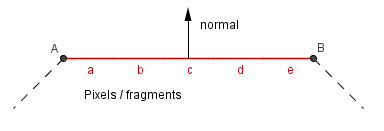
\includegraphics[width=1\linewidth]{flatShading.png}

   \caption{Example of the normal vector being the same across all points on the same face of the mesh. Taken from CGLearn \cite{cglearn}.}
   \label{fig:flat}
\end{figure}

As a result, each face on a model's mesh would appear strictly the same color. The edges between neighboring faces can be clearly seen as long as both neighbors do not lie on the same plane.

GLSL shaders in ThreeJS have two parts, one running after the other while passing information in a sequential manner. The first part is the vertex shader that runs once per vertex in the mesh that is being drawn. The role of the vertex shader is to make vertex calculations based off of the information on that particular vertex, while passing the resulting information onto the next part. The second part is then the fragment shader which runs once per screen pixel the model must be displayed on. This part must take in all of the information that was passed from the vertex shader and calculate the final color of that particular pixel. Because ThreeJS uses vertex shaders, as opposed to surface shaders, the computer only knows the normal vectors of each vertex instead of each face. However, ThreeJS automatically interpolates vertex positions across the entire surface of the mesh. Therefore, we can derive the face normal from the cross product between the derivatives of interpolated positions, $p$, along the $x$ and $y$ directions of the view-space, as shown in \cref{eq:flat-norms}.

\begin{equation}
    \frac{\partial p}{\partial x} \times \frac{\partial p}{\partial y}
    \label{eq:flat-norms}
\end{equation}

\subsection{Gouraud Shading}

This shading technique introduces another system of determining model normal vectors. Instead of generalizing entire faces to the same normal vector, Gouraud shading uses the normal vectors of vertices to calculate the final color of each vertex \cite{wiki:Shading}. The faces that are between the vertices are then colored by linearly interpolating the colors from their surrounding vertices \cite{cglearn}, as shown in \cref{fig:gouraud}.

\begin{figure}[t]
  \centering
  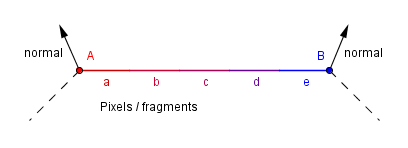
\includegraphics[width=1\linewidth]{gouraudShading.png}

   \caption{Example of vertices having their own color based off of vertex normals. Colors are then interpolated across the face between vertices. Taken from CGLearn \cite{cglearn}.}
   \label{fig:gouraud}
\end{figure}

Resulting images of Gouraud shading seem to be more "smoothly" shaded than images of Flat shading. The one disadvantage of Gouraud shading is that the mesh edges have a more distinct color than the faces. This is due to the colors of pixels lying on mesh edges only having to linearly interpolate between the two colors of the vertices the edge connects while other pixels must derive their colors from more than two vertices.

Since ThreeJS already calculates vertex normals and interpolates colors between vertices by default, implementing Gouraud shading was simply a matter of computing the Lambertian lighting factor \cite{wiki:Lambertian_reflectance} and applying the resulting color to each vertex.

\subsection{Phong Shading and Lighting}

Not only does this shading technique introduce yet another system of determining surface normal vectors, it also acts as a new lighting system \cite{cglearn}. Phong shading aims to create more photorealistic results and improves upon Flat and Gouraud shading by first interpolating the vertex normals themselves across the surface of the mesh, as shown in \cref{fig:phong}. This means that each pixel ultimately gets its own normal vector which can then be used to calculate its own Lambertian lighting factor \cite{wiki:Lambertian_reflectance}, independent from face or vertex normals. This results in an even "smoother" looking result.

\begin{figure}[t]
  \centering
  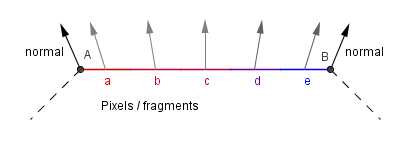
\includegraphics[width=1\linewidth]{phongShading.png}

   \caption{Example of interpolated vertex normals across the mesh surface. Taken from CGLearn \cite{cglearn}.}
   \label{fig:phong}
\end{figure}

Secondly, to add even more photorealism, Phong shading sums up the colors calculated from three different light calculations. Not only does Phong shading take into account Lambertion (or diffuse) lighting, but also blends in colors from ambient and specular lighting. We define ambient light as a color that every item in the environment should be colored in unconditionally as a baseline. We then define specular light as how much the reflected light bounces directly to the viewer, as shown in \cref{fig:phong-angles}. Consider an arbitrary point on the surface of a mesh with its own surface normal vector, $n$, and an incident light vector, $l$. If we define $r$ as the vector representing the reflection of $l$ on $n$ and $v$ as the vector from the point on the surface to the viewer or camera, the following expression can be used to calculate the degree of specular light:

\begin{equation}
    \begin{cases}
         max(r \cdot v, 0) &\text{if } max(n \cdot l, 0) > 0\\
         0 &\text{otherwise}
    \end{cases}
    \label{eq:specular}
\end{equation}

\begin{figure}[t]
  \centering
  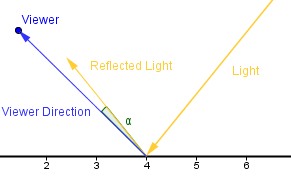
\includegraphics[width=0.65\linewidth]{angles1.png}

   \caption{Example of reflected light heading towards the viewer. Taken from CGLearn \cite{cglearn}.}
   \label{fig:phong-angles}
\end{figure}

Once the ambient, diffuse, and specular light values have been summed up, the resulting drawing of the model not only looks smooth, but also "shiny" in areas facing towards the light source, as shown in \cref{fig:phong-lighting}. The scalar result of this expression in \cref{eq:specular} is often raised to a power to lessen the area the area that "glistens" due to specular lighting.

\begin{figure}[t]
  \centering
  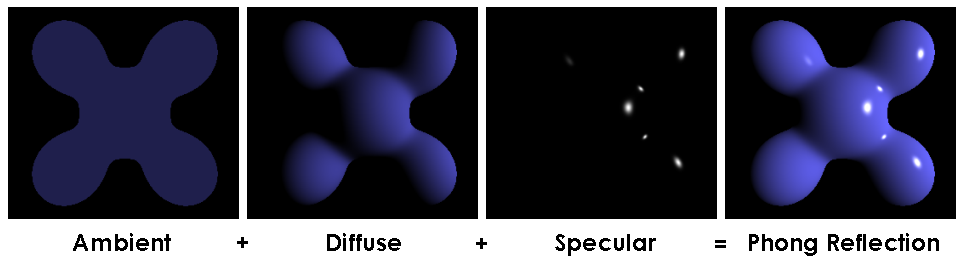
\includegraphics[width=1\linewidth]{Phong_components_version_4.png}

   \caption{Example of combining the lighting components in Phong shading. Taken from Wikipedia \cite{wiki:Phong_shading}.}
   \label{fig:phong-lighting}
\end{figure}

\subsection{Cel Shading}

Apart from the previously aforementioned shading techniques, Cel shading aims to create more cartoon-ish and nonphotorealistic results. We use Cel shading as our first step towards Anime-like depictions of 3D models. As mentioned before, Cel shading summarizing areas that have similar colors as single shades \cite{wiki:Cel_shading}. Our implementation of Cel shading summarizes possible values of Lambertian lighting factors into five distinct categories covering equal ranges each, resulting in five different summary values. The implementation follows the expression found below:

\begin{equation}
    \begin{cases}
         1 &\text{if } (n \cdot l) * 0.5 + 0.5 > 0.8\\
         0.75 &\text{if } (n \cdot l) * 0.5 + 0.5 > 0.6\\
         0.5 &\text{if } (n \cdot l) * 0.5 + 0.5 > 0.4\\
         0.25 &\text{if } (n \cdot l) * 0.5 + 0.5 > 0.2\\
         0 &\text{otherwise}
    \end{cases}
    \label{eq:cel}
\end{equation}

As a result, models that are Cel shaded are only drawn with a limited palette of colors. This makes the model seem more "flat" than 3D. 

\subsection{Silhouette Drawing}

As we move towards the goal of drawing 3D models in a cartoon-ish Anime-like manner, the ability to draw lines onto the model become more important. We use silhouette drawing as means to mimic the overall cartoon style since we find that objects in cartoons likely show their own outlines along with its coloring. Since ThreeJS allows for the rendering of one scene on top of another, our work uses this as means to do multiple passes on the same object. Our implementation for silhouette drawing is split into two passes:

\begin{itemize}
    \item The first pass perturbs the model's mesh along its vertex normals and shades the model as one solid color.
    \item The second pass shades its own copy of the mesh using Cel shading on top of the first pass.
\end{itemize}

The first pass simply lays down a slightly bigger shape so that it can be covered by the Cel shaded second pass. The resulting render would then include both the Cel shaded model and a small outline around the area, depicting the edges of the figure in the image.

\subsection{Contour Line Drawing}

While we aim to have models appear less 3D, we still want to mimic an artists portrayal of a 3D object. Just as an artist would draw contour lines to convey shape, we implement our shaders to do the same. Given an arbitrary point on the surface of a model, we define the point to be a contour if the dot product between the surface normal, $n$, and its vector towards the viewer, $v$, is equal to zero, namely:

\begin{equation}
    n \cdot v = 0
    \label{eq:contour}
\end{equation}

This implies that at such points, the normal vector is directly perpendicular to the vector that is directed towards the viewer. This means that to the viewer, the point is on a crease of the surface to which the viewer cannot see the other side of. If these points are colored differently, they can potentially form a contour line as shown in \cref{fig:contour}.

\begin{figure}
    \centering
    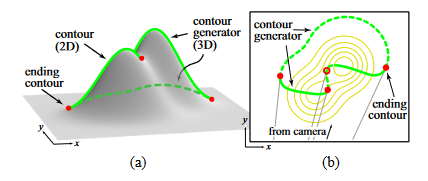
\includegraphics[width=1\linewidth]{contours.png}
    \caption{(a) Example of a contour line being projected to an image. (b) A topological map of the surface shown in (a) with the contour line drawn relative to the camera. Taken from DeCarlo \etal \cite{DeCarlo:2003:SCF}.}
    \label{fig:contour}
\end{figure}

The only caveat to this is that when calculating the dot products between $n$ and $v$ for each pixel, the pixels that were meant to be a part of the contour line did not have dot products of exactly zero. Thus, we add flexibility to the condition stated in \cref{eq:contour}, counting pixels whose dot product values fall between a certain range around zero as part of the contour as well. This results in thicker, more continuous contour lines that effectively convey the model's shape even when it is drawn like a cartoon.

\subsection{Suggestive Contour Line Drawing}

The final shading technique we implement proves to be a bit more complex than the rest. In addition to contour lines, we look to also include suggestive contour lines to increase expressiveness of the original shape of the model. Suggestive contours are a bit harder to define, so we follow the definition as stated by DeCarlo \etal\cite{DeCarlo:2003:SCF} as follows:

\begin{equation}
    D_w(n \cdot v) = 0 \text{,\quad and}
    \label{eq:sugg1}
\end{equation}

\begin{equation}
    D_w(D_w(n \cdot v)) > 0
    \label{eq:sugg2}
\end{equation}

The conditions from \cref{eq:sugg1} and \cref{eq:sugg2} denote the local minima of the dot product, $n \cdot v$, in the direction of a new vector, $w$. Given an arbitrary point on the surface of a model, let $n$ be the surface normal of that point and $v$ be the vector from that point to the viewer. Then $w$ is the projection of $v$ onto the plane defined by $n$, namely the tangent plane of that point on the surface as shown in \cref{fig:tangentplane}.

\begin{figure}
    \centering
    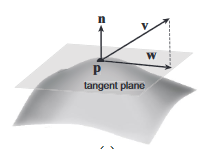
\includegraphics[width=0.6\linewidth]{tangentplane.png}
    \caption{Example $w$ vector from projecting $v$ onto the tangent plane defined by $n$. Taken from DeCarlo \etal\cite{DeCarlo:2003:SCF}.}
    \label{fig:tangentplane}
\end{figure}

Calculating $D_w(n \cdot v)$ is quite simple in GLSL since the language offers functionality to compute derivatives of certain expressions based off of finite differences between neighboring pixels in the $x$ and $y$ directions of the view space. We calculate $w$ by using the following equation:

\begin{equation}
    w = v - ((n \cdot v) \cdot n)
    \label{eq:w}
\end{equation}

We then use the $w$ from \cref{eq:w} to calculate $D_w(n \cdot v)$ by this following formula based on the definition of the directional derivative:

\begin{equation}
    (\nabla (n \cdot v)) \cdot \frac{w}{||w||}
    \label{eq:first}
\end{equation}

We note that even though the $w$ vector is 3-dimensional, we can only take the derivative of $n \cdot v$ in only the $x$ and $y$ directions of the view-space. So, we assume that the derivative of $n \cdot v$ is zero in the $z$ direction since there should be no difference in the dot product as we move along $z$. Moving along $z$ implies jumping off of the surface of the model, therefore we choose to neglect such values in our calculations.

Taking the second degree directional derivative proved to be a bit trickier since GLSL did not have the functionality to calculate higher order derivatives. While we would have liked to implement this shading technique on GLSL because of its support for GPUs, we had to move a portion of our implementation to Python since it allows us to access information pertaining to neighboring pixels. With calculations being split across the two seperate platforms, we needed some way for the two parts to communicate. Thus, we implement another multipass approach:

\begin{itemize}
    \item The first pass outputs a texture based on the normal vectors of the model's surface.
    \item The second pass outputs a texture based on the vectors from each pixel to the viewer.
    \item The third pass outputs a texture based on the $w$ vectors calculated from the $n$ and $v$ vectors at each pixel.
    \item The final pass takes all the results from the previous passes and calculates which pixels should be drawn as a suggestive contour based on the finite differences between neighboring pixels.
\end{itemize}

The only pass that must be computed in Python is the fourth and final pass, while all other passes can be done by the GLSL side. This final pass calculates the first order directional derivative by finding the following forward finite difference of $n \cdot v$:

\begin{equation}
    D_w(n \cdot v) = 
    \begin{pmatrix}
        n_{x+1} \cdot v_{x+1} - n \cdot v\\
        n_{y+1} \cdot v_{y+1} - n \cdot v
    \end{pmatrix}
    \cdot \frac{w}{||w||}
    \label{eq:first-python}
\end{equation}

We can then define the second order derivative as the following backward finite difference of $D_w(n \cdot v)$:

\begin{equation}
    D_w^2(n \cdot v) = 
    \begin{pmatrix}
        D_w(n \cdot v) - D_w(n_{x-1} \cdot v_{x-1})\\
        D_w(n \cdot v) - D_w(n_{y-1} \cdot v_{y-1})
    \end{pmatrix}
    \cdot w
    \label{eq:second-python}
\end{equation}

By using the expressions found in \cref{eq:first-python} and \cref{eq:second-python}, we only need to access directly adjacent neighbors surrounding the pixel we are calculating derivatives of. We run this calculation on all pixels that are not on the edge of the image, taking into account the $w$, $v$, and $n$ vectors for each pixel, in order to determine which pixels should be drawn as a suggestive contour. Just like in drawing regular contour lines, some derivative values do not fit the exact conditions from \cref{eq:sugg1} and \cref{eq:sugg2}. Thus, we set a range around the correct values to allow for flexibility, resulting in thicker, more continuous suggestive contour lines. We show an example of outputs of the three intermediary passes of our implementation of suggestive contour shading on the Stanford Lucy in \cref{fig:lucy-python}.

\begin{figure}
  \centering
  \begin{subfigure}{.88\linewidth}
    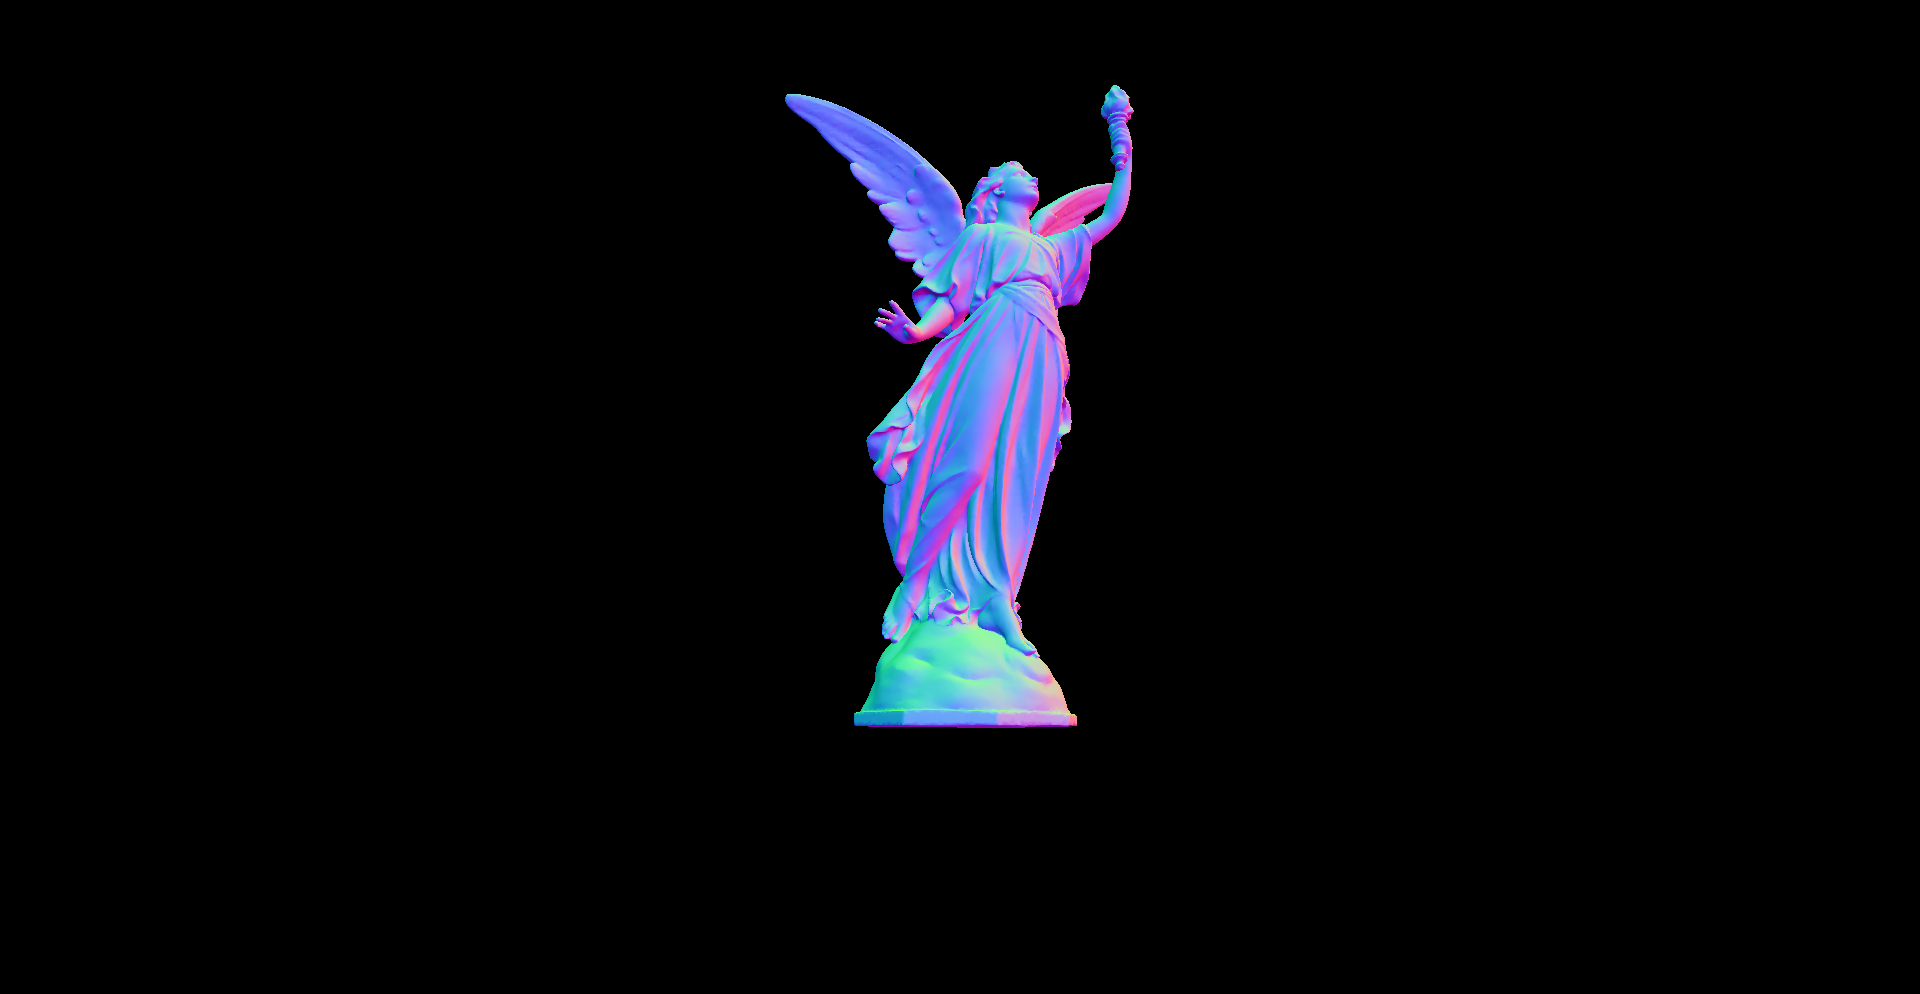
\includegraphics[width=1\linewidth]{lucy/normals.png}
    \caption{Example output from first pass, with normal vectors shown.}
    \label{fig:lucy-normals}
  \end{subfigure}
  \hfill
  \begin{subfigure}{.88\linewidth}
    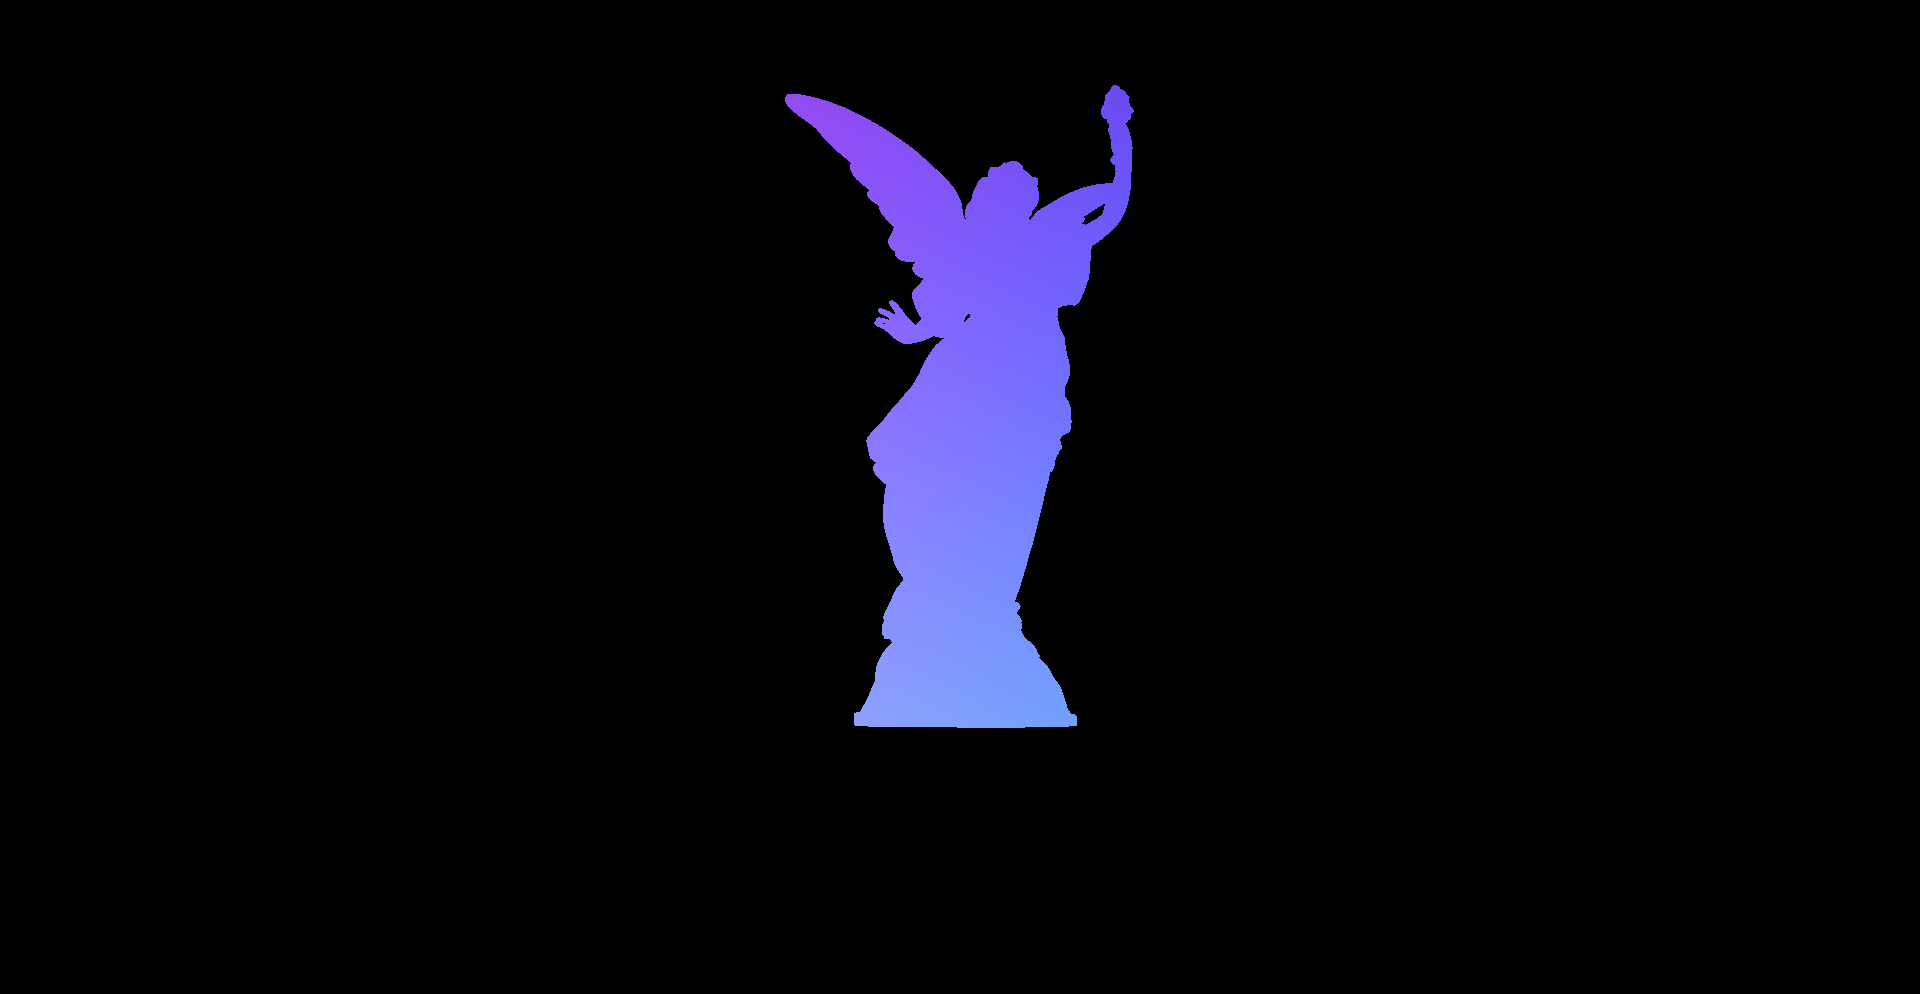
\includegraphics[width=1\linewidth]{lucy/viewers.png}
    \caption{Example output from second pass, with view vectors shown.}
    \label{fig:lucy-views}
  \end{subfigure}
  \hfill
  \begin{subfigure}{0.88\linewidth}
    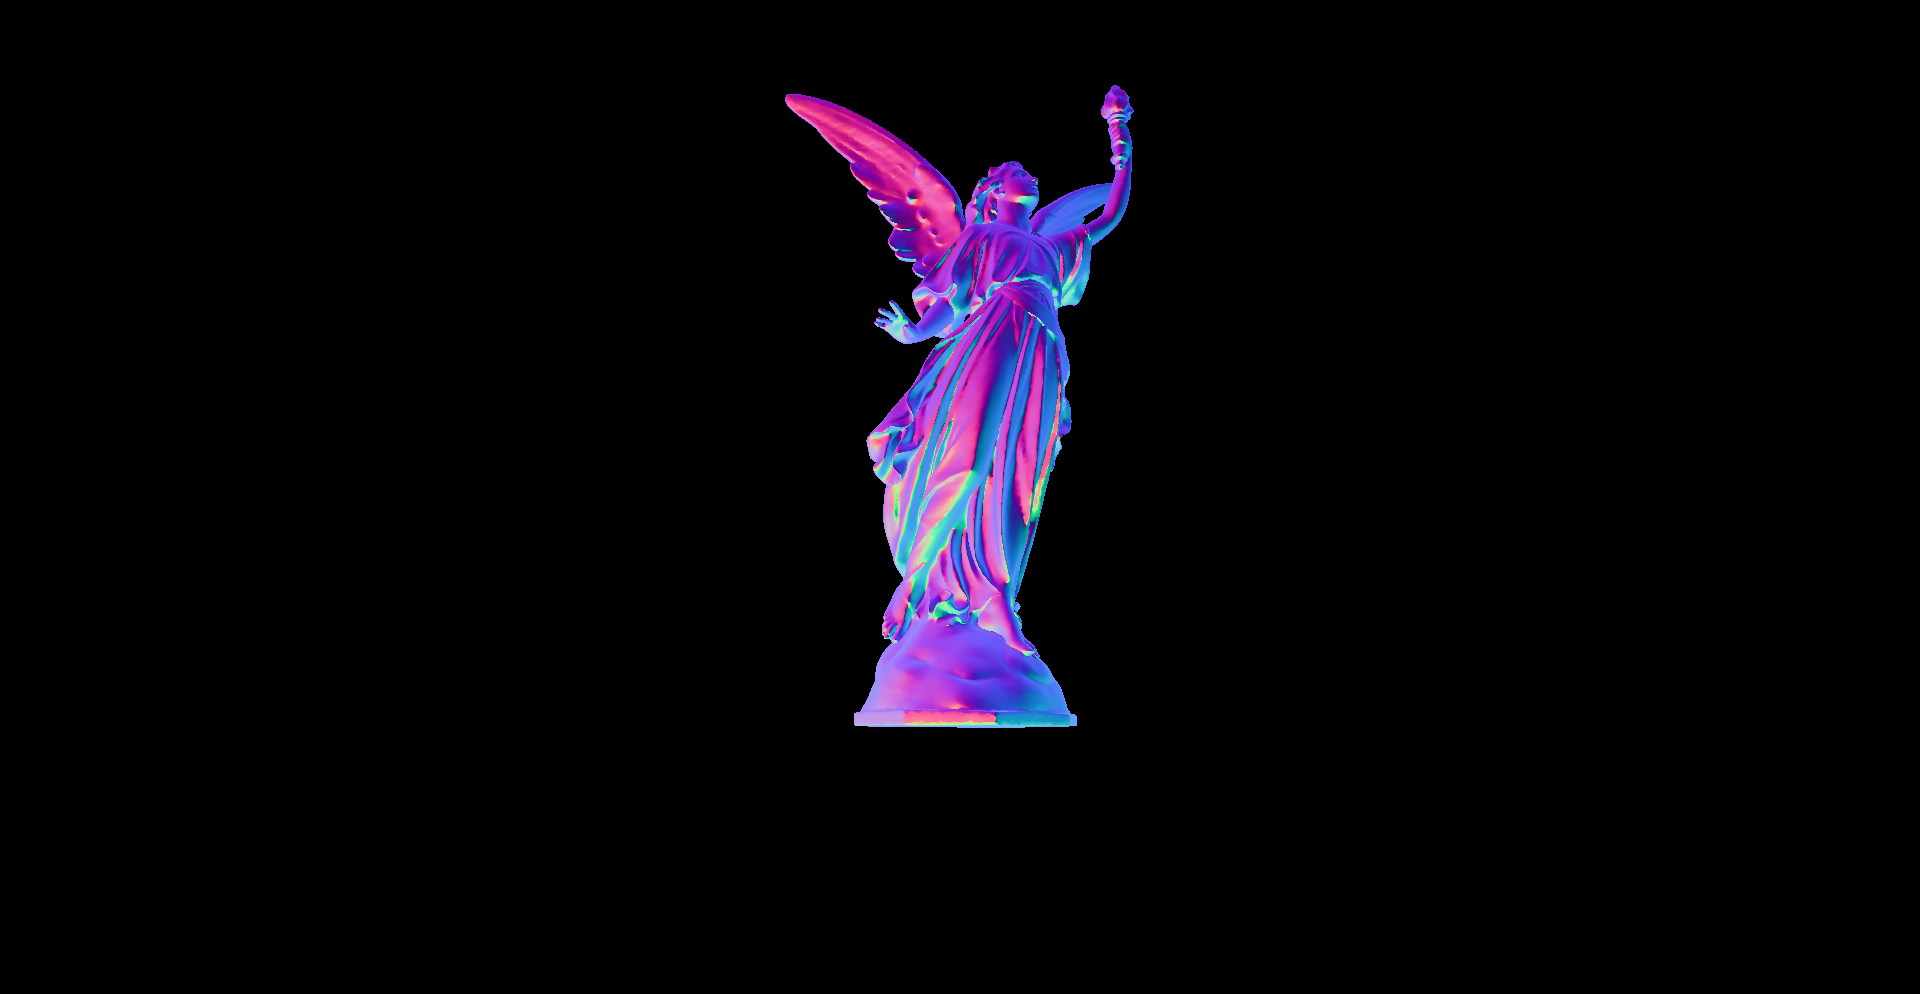
\includegraphics[width=1\linewidth]{lucy/ws.png}
    \caption{Example output from third pass, with $w$ vectors shown.}
    \label{fig:lucy-ws}
  \end{subfigure}
  \caption{Outputs from the intermediate passes for calculating suggestive contours. These passes were run on the Stanford Lucy model.}
  \label{fig:lucy-python}
\end{figure}

With the implementations of all the previously mentioned shading techniques complete, we combine all of the nonphotorealistic shaders together to achieve our goal of depicting 3D models in an Anime-like style.

%-------------------------------------------------------------------------
\section{Results}
\label{sec:results}

We first show the results of our classical shaders on more basic 3D shapes that are provided to us by default from the ThreeJS library. Since ThreeJS also includes its own proprietary classical shaders, we show a comparison between the results from our implementation and their implementations. We then move on to show the effects of each of our nonphotorealisitic shaders individually before combining all of them together. We decided to show our nonphotorealistic shaders on more complex 3D models since they are more detailed than the simple shapes ThreeJS includes by default, making them more likely to have contours and suggestive contours on any given angle of view. We also wanted these 3D models to have as high of a polygon count as possible so that our shader thresholds would work better for them.


As demonstrated in \cref{fig:flat-sphere}, \cref{fig:flat-tk}, and \cref{fig:flat-tea}, flat shading only shades the 3D shape based on the normals of the faces in its mesh, making all of the pixels in each face of the model share the same color. This results in flat shading giving the models the simplest look. In \cref{fig:gouraud-sphere}, \cref{fig:gouraud-tk}, and \cref{fig:gouraud-tea}, we show that because its dependence on vertex normals, the results of Gouraud shading display the vertices and edges of a mesh faintly different from the rest of the model's surface. However, this issue is lessened if the polygon resolution of the model is increased, since there would be more edges and vertices to blend colors in with. Even with its disadvantages, Gouraud shading still gives a much smoother look to the model than flat shading. We further improve this smoothness with Phong-interpolated normals, as seen in \cref{fig:lambert-sphere}, \cref{fig:lambert-tk}, and \cref{fig:lambert-tea}. With interpolated vertex normals, each pixel no longer needs to depend on the color of its neighboring vertices since each pixel will have its own normal vector to calculate its own color. This rids of the disadvantages of only using vertex normals as Gouraud shading does while under the same Lambertion lighting system. We show that we can add another flavor to the 3D models by using Phong shading, as displayed in \cref{fig:phong-sphere}, \cref{fig:phong-tk}, and \cref{fig:phong-tea}. With Phong lighting, shininess of objects can be simulated by adding in both specular and ambient light calculations, making the models look even more photorealistic. When comparing our implementations against the ThreeJS library, we show that were able to accurately reproduce the results that ThreeJS achieves with its shaders with the exception of our Phong shader. Though we were not able to mimic the exact "shine" of the resulting renders of the ThreeJS implementation, we were still able to replicate a shine that remains loyal to the purpose of the Phong reflection model \cite{wiki:Phong_shading}.

In \cref{fig:lucy} and \cref{fig:ajax}, we show the effects of each nonphotorealistic shader we implemented. We then combine all of their respective effects together to try to replicate the model's appearance in a cartoon-ish context. We finally test out our nonphotorealistic strategy to more complex models, including models inspired by popular Anime culture, to see whether our results replicate an Anime-like style. Since final result of including suggestive contours draws extra lines on the character's face, we show the difference between including and excluding suggestive contours, as seen in \cref{fig:lucy-compare}, \cref{fig:ajax-compare}, \cref{fig:amber-compare}, and \cref{fig:pekora-compare}. We also test our nonphotorealistic shading techniques on a model of Amber from the game Genshin Impact and of Pekora Usada, a Hololive virtual YouTuber. Since both of these models are based off of Anime-styled characters, we tried our shaders on these characters to see if we have successfully mimicked the Anime-style 2D depiction.

%------------------------------------------------------------------------
\section{Conclusion \& Future Work}
\label{sec:conclusion}

While we have shown implementations for nonphotorealistic shading in ThreeJS, GLSL, and Python, we could have improved our implementations even further. We were not able to completely implement our suggestive contour shader \cite{DeCarlo:2003:SCF} on the ThreeJS platform due to limited access to data on neighboring pixels. Because of our decision to move to Python to support this shader, we lost the advantage of GPU parallelism for certain parts of the implementation. In order to load the results from the previous passes to Python for it to calculate suggestive contours, we import the images one by one, pixel by pixel. Even the calculations that are done in Python are also computed pixel by pixel. This process proves to be highly inefficient and not ideal. We look to the Python library, NumPy, to optimize the storing of image information since the data structures included in that library are highly optimized for large amounts of data that are of the same type. We can look toward further improving our implementation by vectorizing the calculations done on the pixel data stored in the NumPy structures since NumPy is heavily optimized for such operations. Future efforts could also be used to discover an implementation for suggestive contours that is based entirely on GLSL.

In conclusion, we provide a study on both classical and nonphotorealistic shading techniques and show each of their effects on various 3D models. We effectively use Cel shading \cite{wiki:Cel_shading} along with silhouette, contour line, and suggestive contour line drawing \cite{DeCarlo:2003:SCF} to mimic the Anime-style depiction and display the combined effects on various models, including a few Anime characters. As a result, we are able to produce images that accurately imitates a cartoon-ish 2D look akin to the overall Anime-style. We have made our shader implementations publicly available at \url{https://github.com/ShuhongChen/anime-shaders}

%%%%%%%%% REFERENCES
{\small
\bibliographystyle{ieee_fullname}
\bibliography{egbib}
}


\setcounter{section}{0}
\renewcommand\thesection{\Alph{section}}
\renewcommand\thesubsection{\thesection.\Alph{subsection}}

\section{Artist Attributions}
\begin{itemize}
    \item ajax.stl: \url{https://cults3d.com/en/3d-model/art/bust-of-ajax}
    \item amber.stl: \url{https://hub.vroid.com/en/characters/3742574954744824945/models/3661281045858685259}
    \item lucy.stl: \url{https://www.thingiverse.com/thing:41939}
    \item usada\_pekora.stl: \url{https://3d.nicovideo.jp/works/td67414}
    \item Utah\_teapot.stl: \url{https://cults3d.com/en/3d-model/art/utah-teapot-solid}
\end{itemize}


%--Sphere--

\begin{figure*}
    \centering
    \begin{subfigure}{.48\linewidth}
        \frame{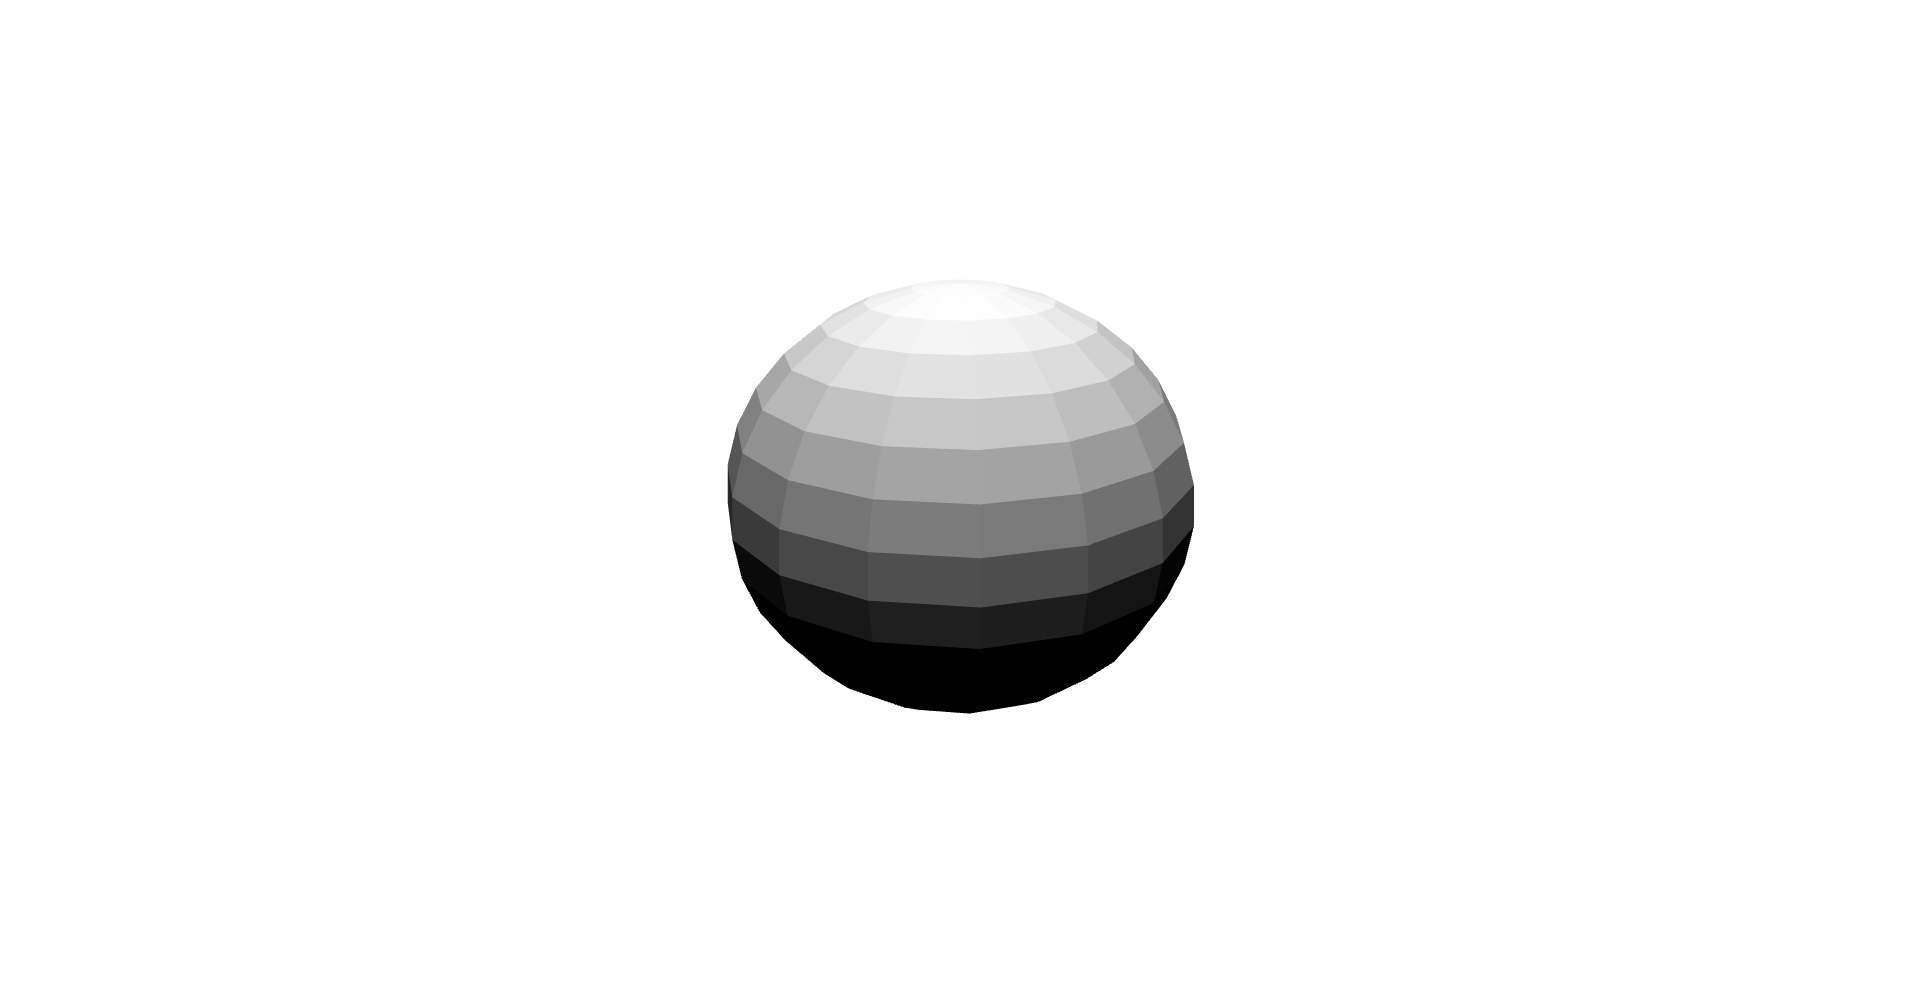
\includegraphics[width=1\linewidth]{sphere/ourFlatSphere.png}}
        \caption{Flat shaded sphere using our implementation.}
        \label{fig:our-flat-sphere}
    \end{subfigure}
    \hfill
    \begin{subfigure}{.48\linewidth}
        \frame{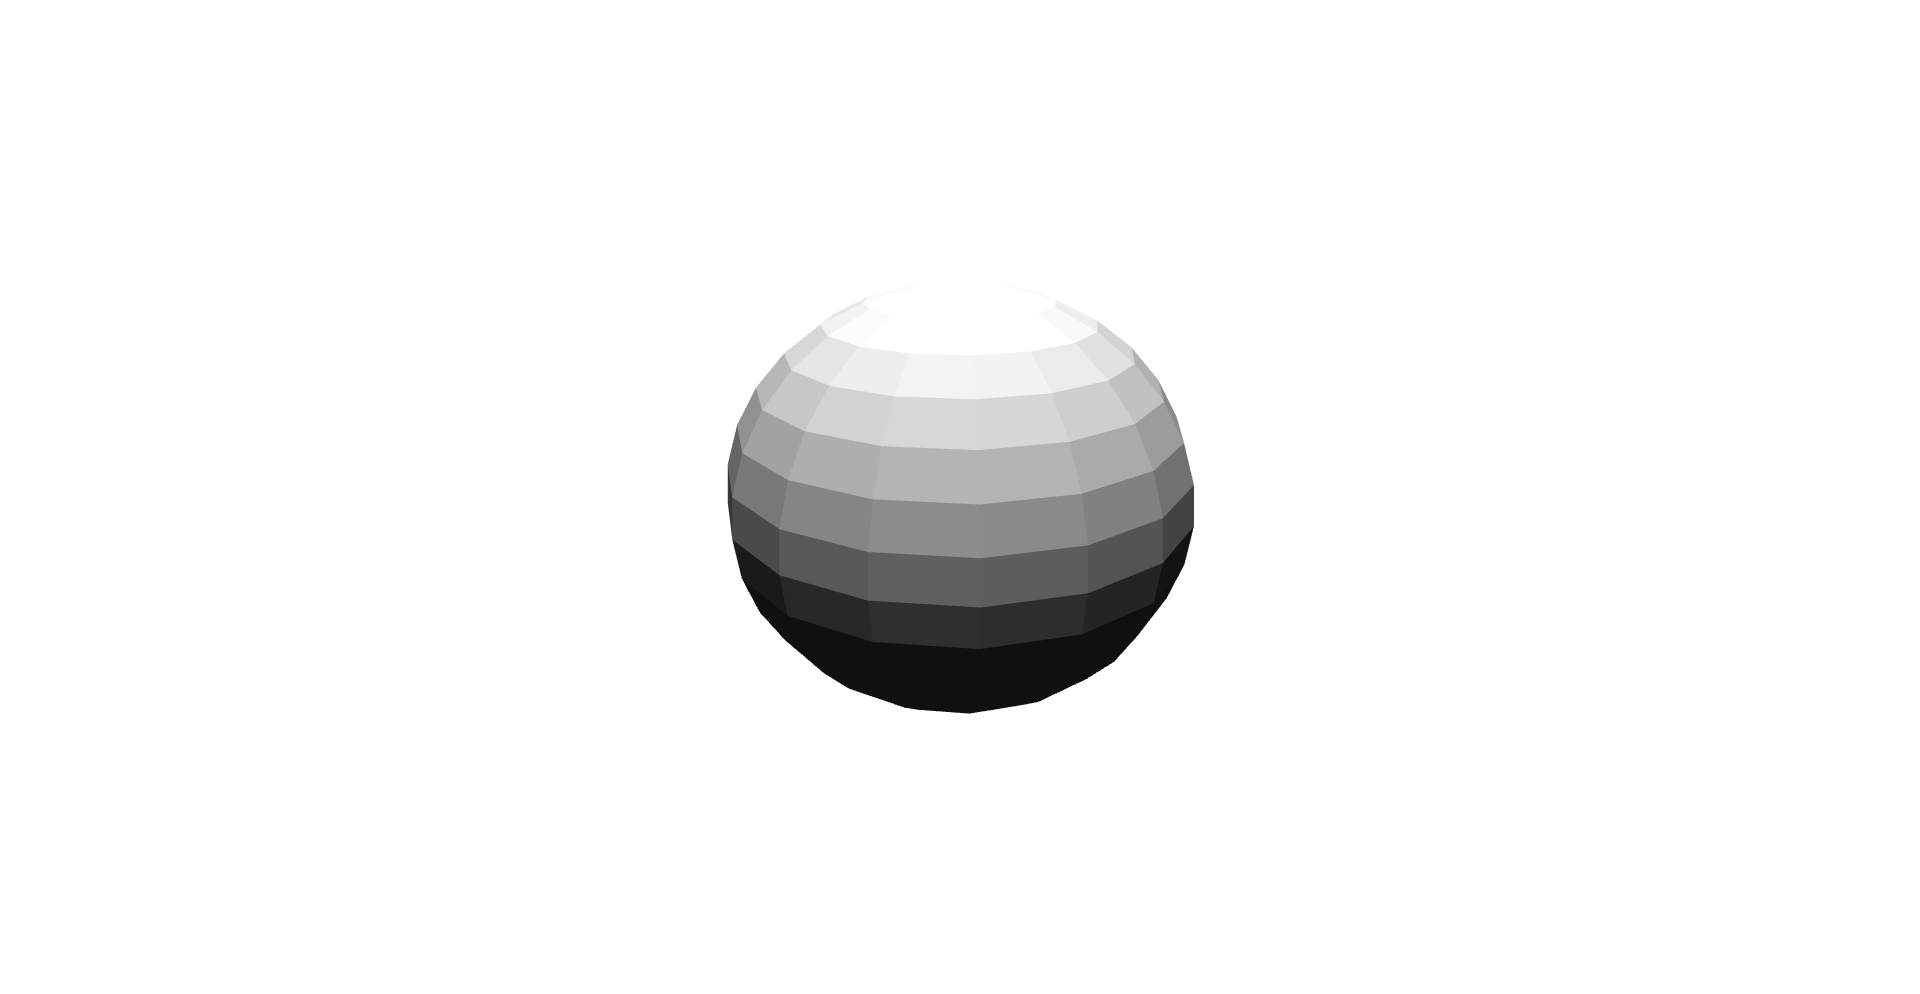
\includegraphics[width=1\linewidth]{sphere/threeFlatSphere.png}}
        \caption{Flat shaded sphere using ThreeJS implementation.}
        \label{fig:three-flat-sphere}
    \end{subfigure}
    \caption{Example of Flat shading on a basic sphere mesh. Because flat shading only uses face normals, the faces of the mesh can be differentiated from each other.}
    \label{fig:flat-sphere}
\end{figure*}

\begin{figure*}
    \centering
    \begin{subfigure}{.48\linewidth}
        \frame{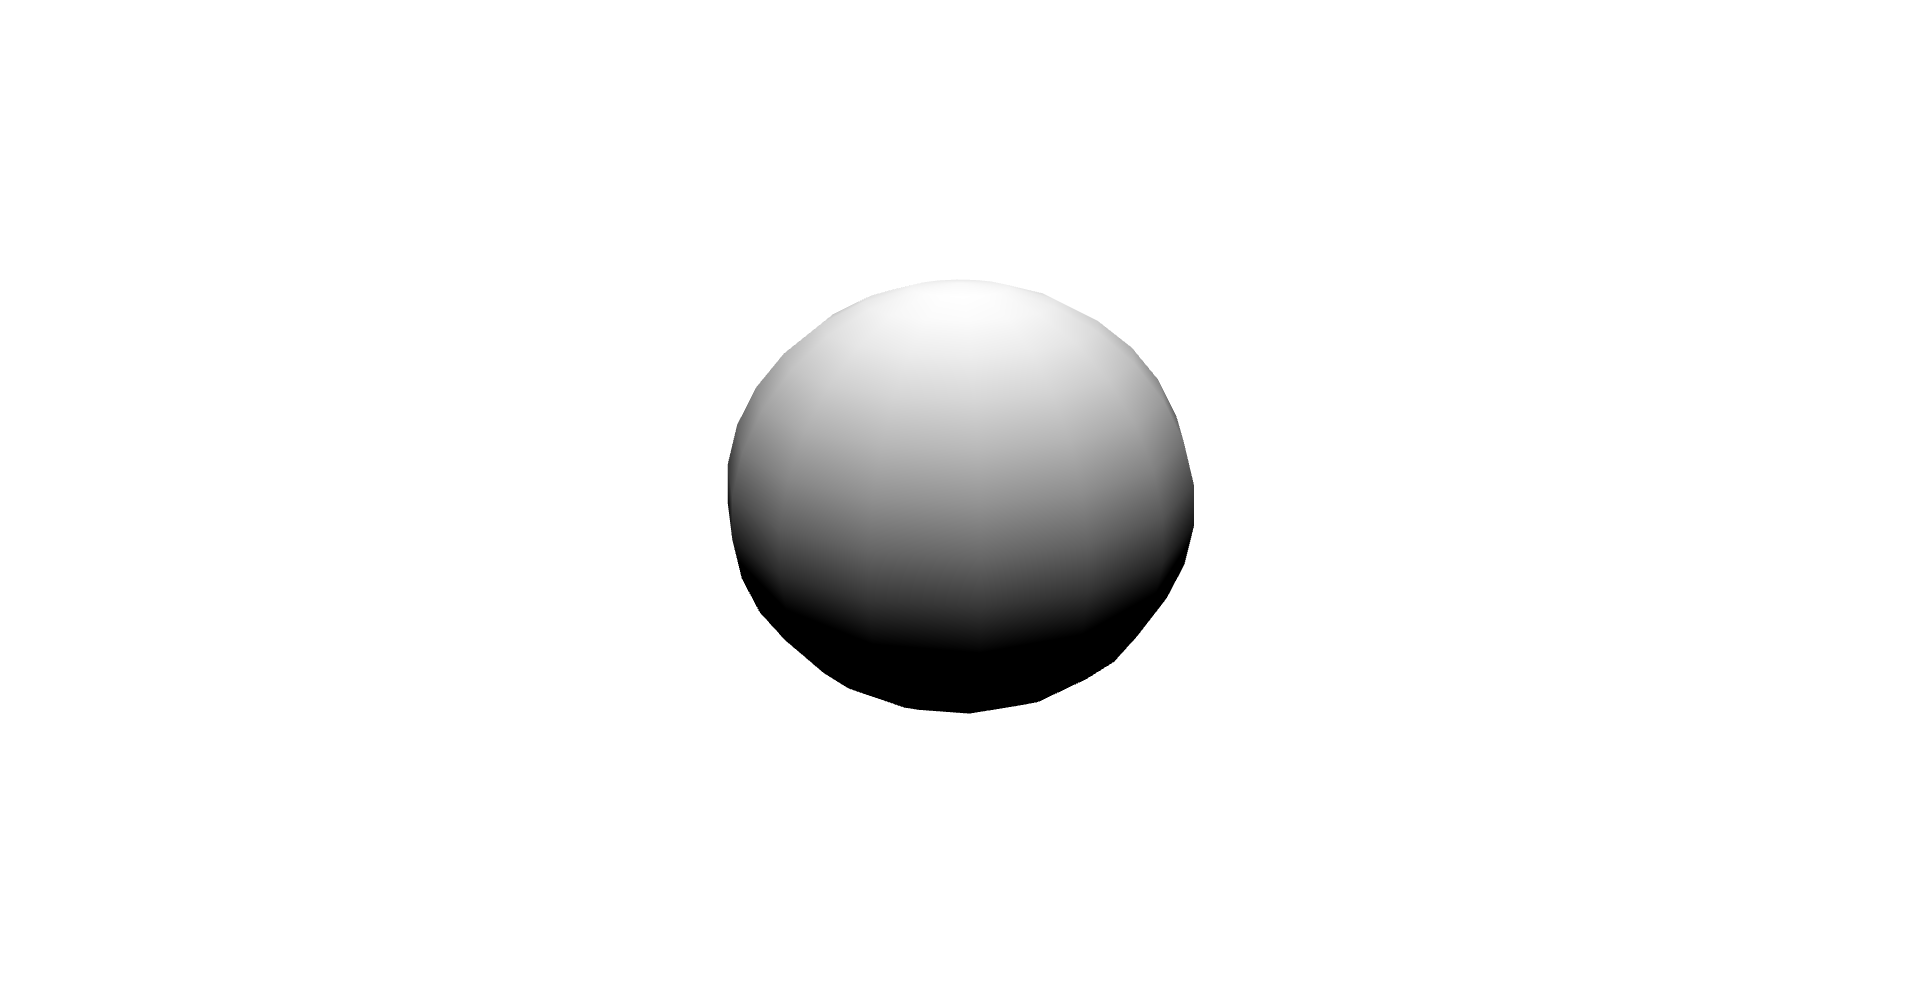
\includegraphics[width=1\linewidth]{sphere/ourGouraudSphere.png}}
        \caption{Gouraud shaded sphere using our implementation.}
        \label{fig:our-gouraud-sphere}
    \end{subfigure}
    \hfill
    \begin{subfigure}{.48\linewidth}
        \frame{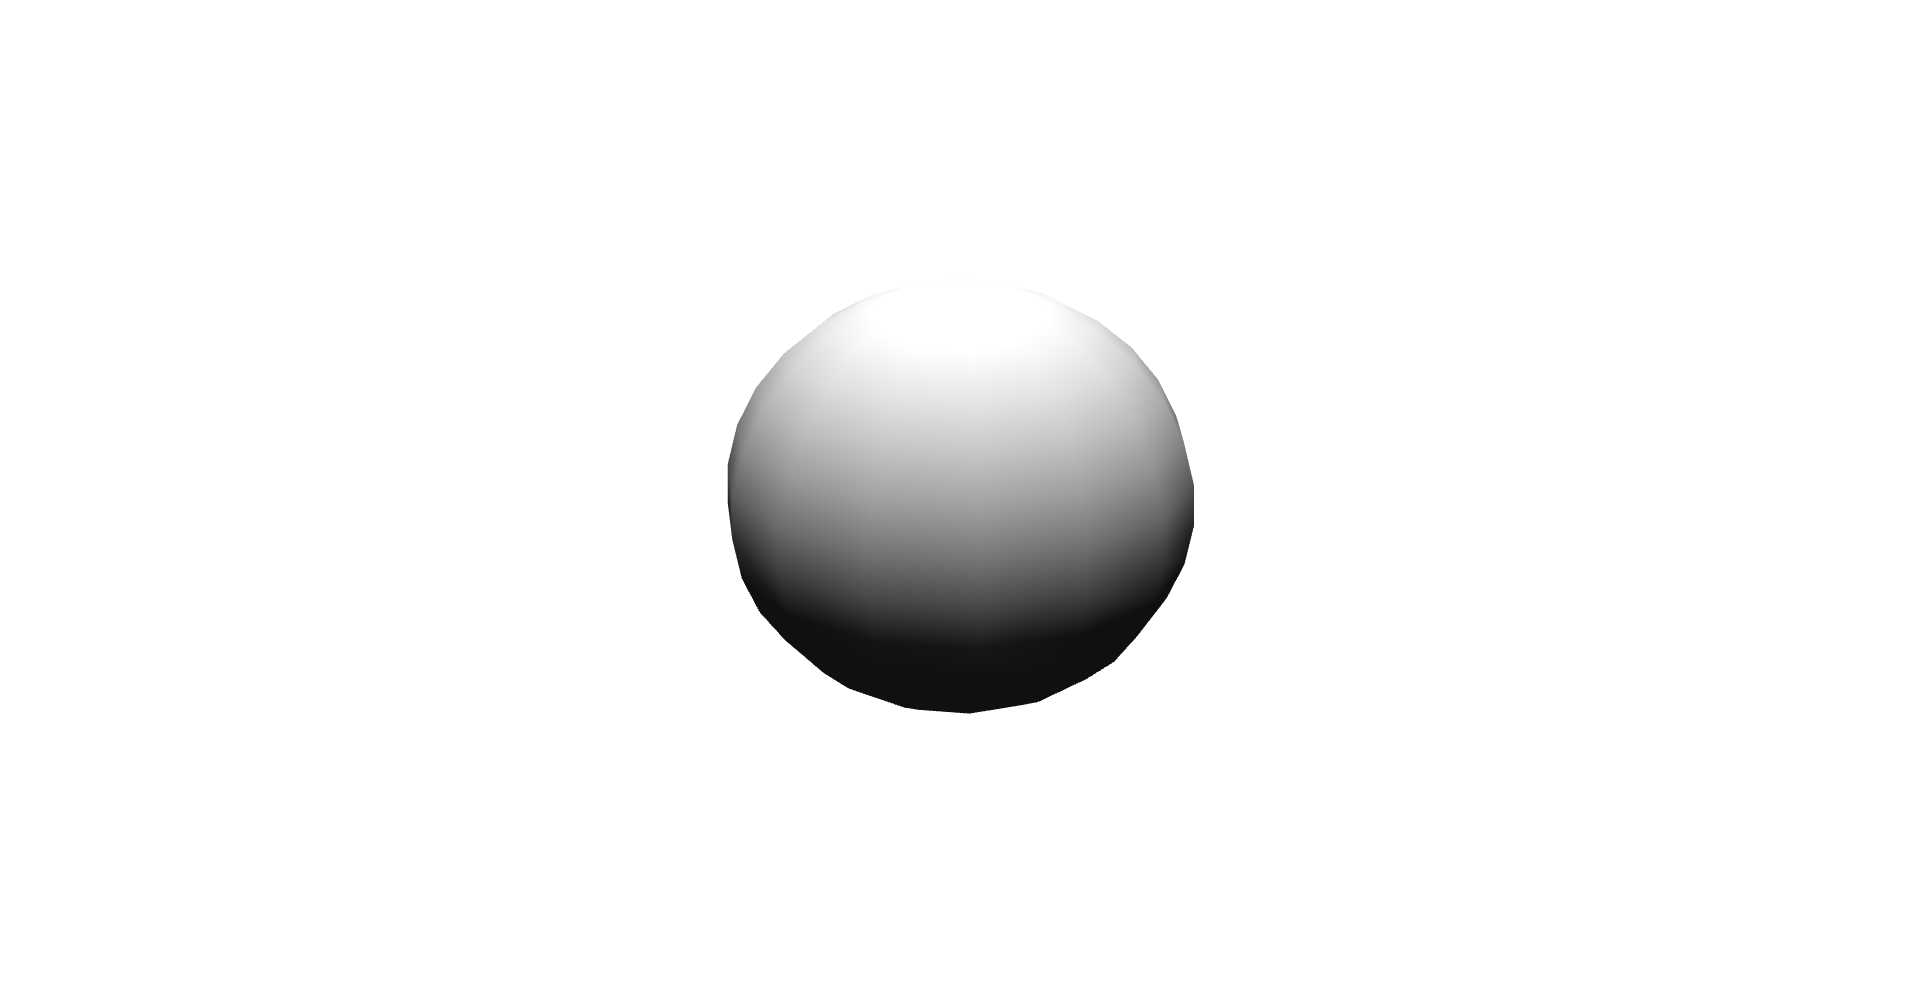
\includegraphics[width=1\linewidth]{sphere/threeGouraudSphere.png}}
        \caption{Gouraud shaded sphere using ThreeJS implementation.}
        \label{fig:three-gouraud-sphere}
    \end{subfigure}
    \caption{Example of Gouraud shading on a basic sphere mesh. Because Gouraud shading only uses vertex normals, the sphere looks "smoother." However, faint white lines along the mesh edges are still apparent since colors are interpolated between vertices. Edge pixels only interpolate between two vertices while face pixels must interpolate between three or more.}
    \label{fig:gouraud-sphere}
\end{figure*}

\begin{figure*}
    \centering
    \begin{subfigure}{.48\linewidth}
        \frame{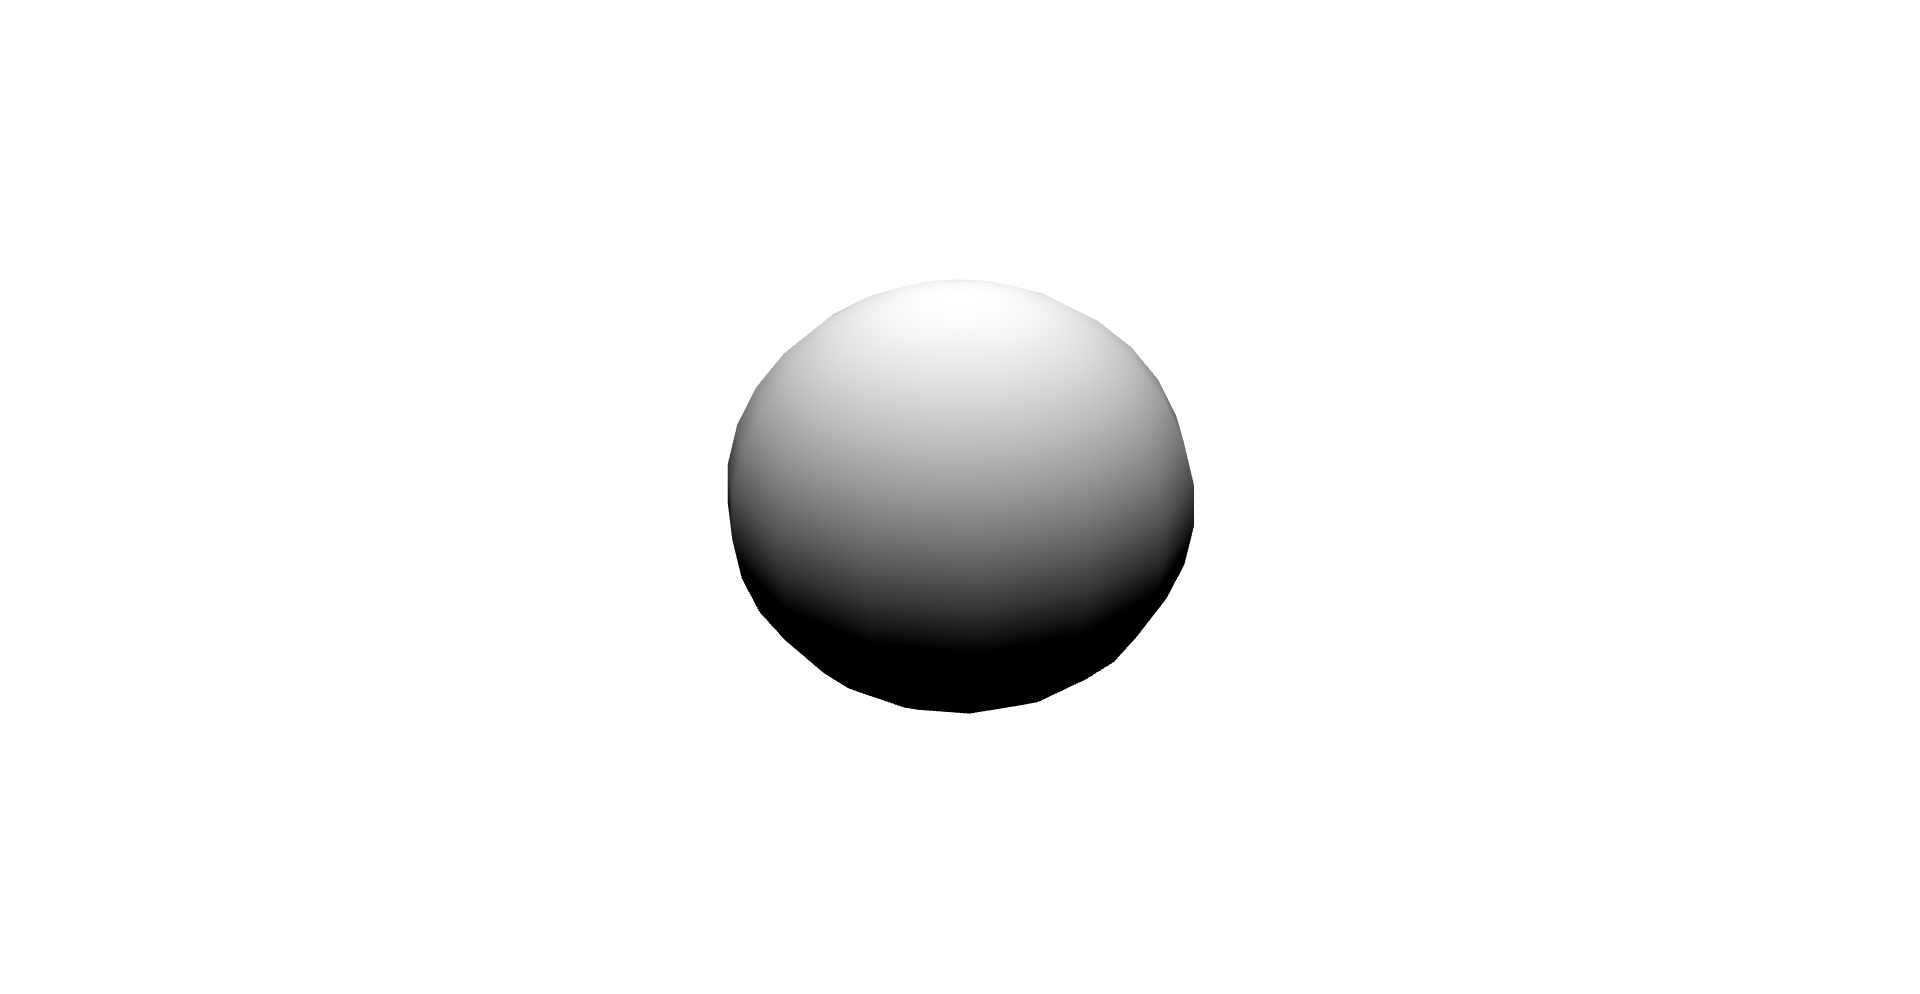
\includegraphics[width=1\linewidth]{sphere/ourLambertSphere.png}}
        \caption{Lambert shaded sphere using our implementation.}
        \label{fig:our-lambert-sphere}
    \end{subfigure}
    \hfill
    \begin{subfigure}{.48\linewidth}
        \frame{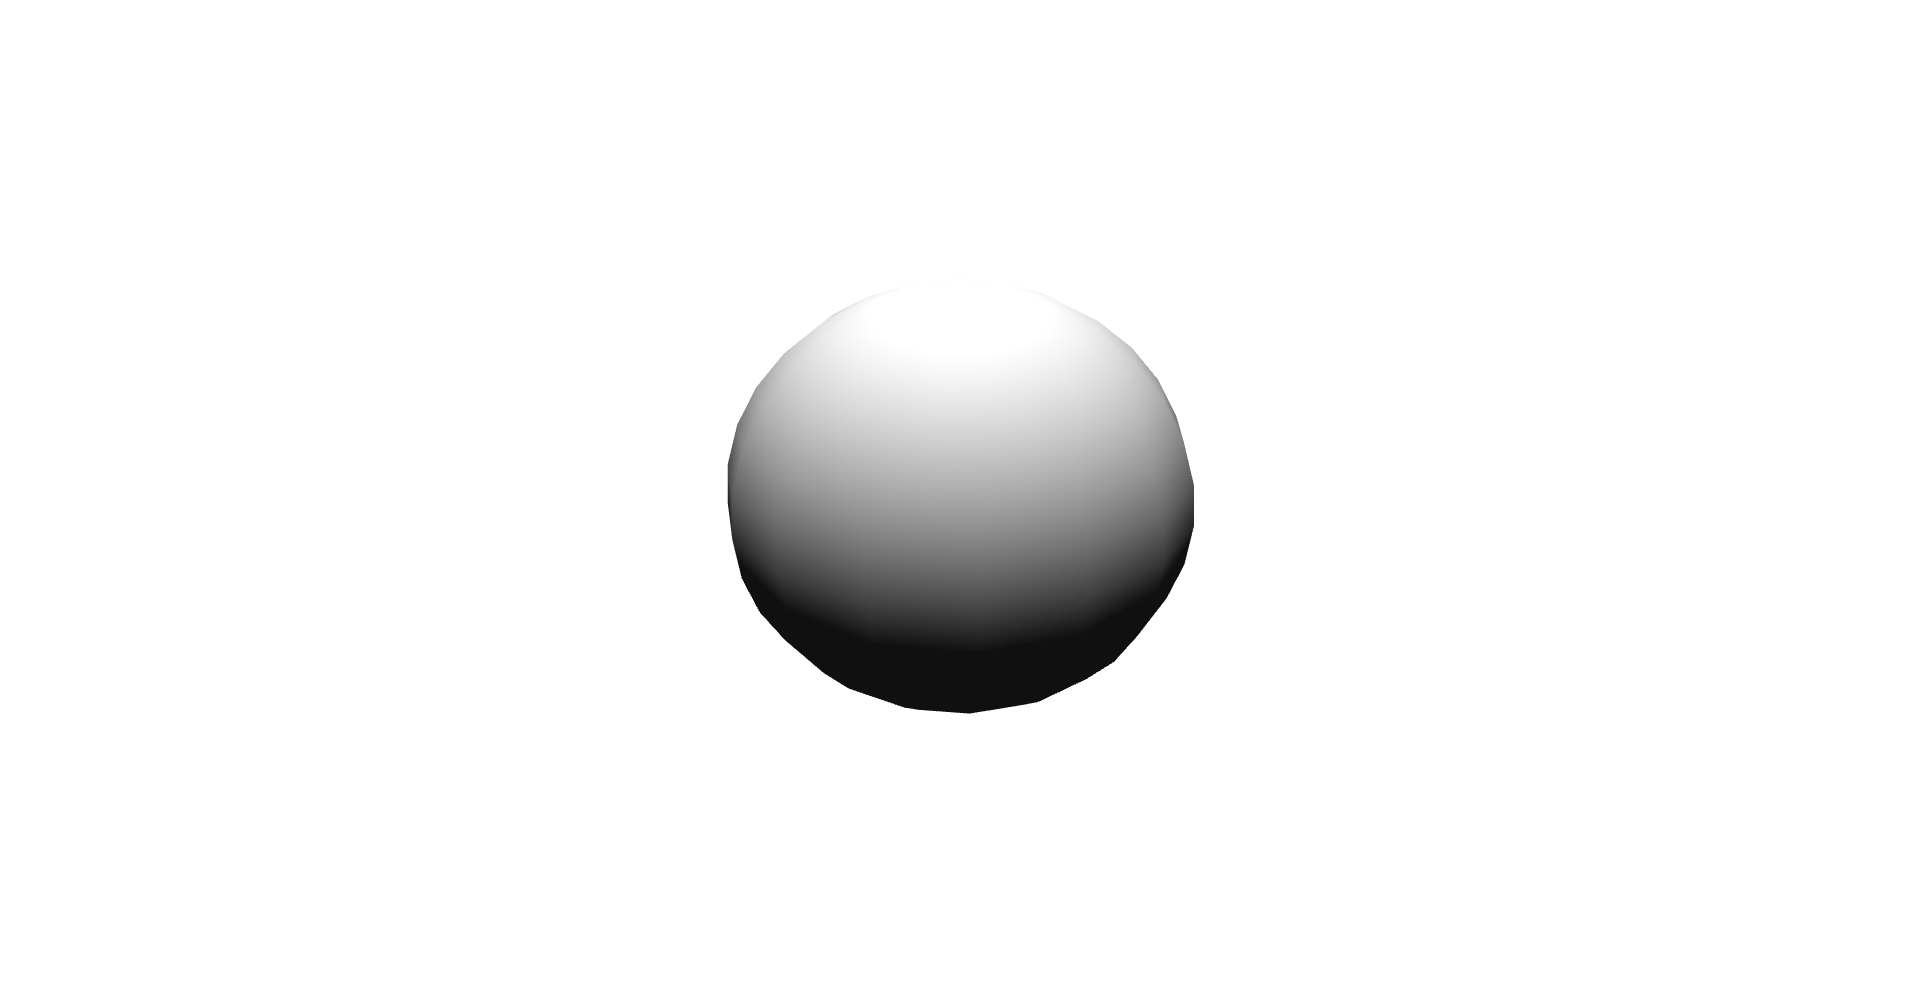
\includegraphics[width=1\linewidth]{sphere/threeLambertSphere.png}}
        \caption{Lambert shaded sphere using ThreeJS implementation.}
        \label{fig:three-lambert-sphere}
    \end{subfigure}
    \caption{Example of Lambert shading on a basic sphere mesh with Phong normals. Since this shader now uses interpolated normal vectors from vertex normals, the color of each pixel no longer relies on the color of neighboring vertices, giving the shape an even "smoother" appearence.}
    \label{fig:lambert-sphere}
\end{figure*}

\begin{figure*}
    \centering
    \begin{subfigure}{.48\linewidth}
        \frame{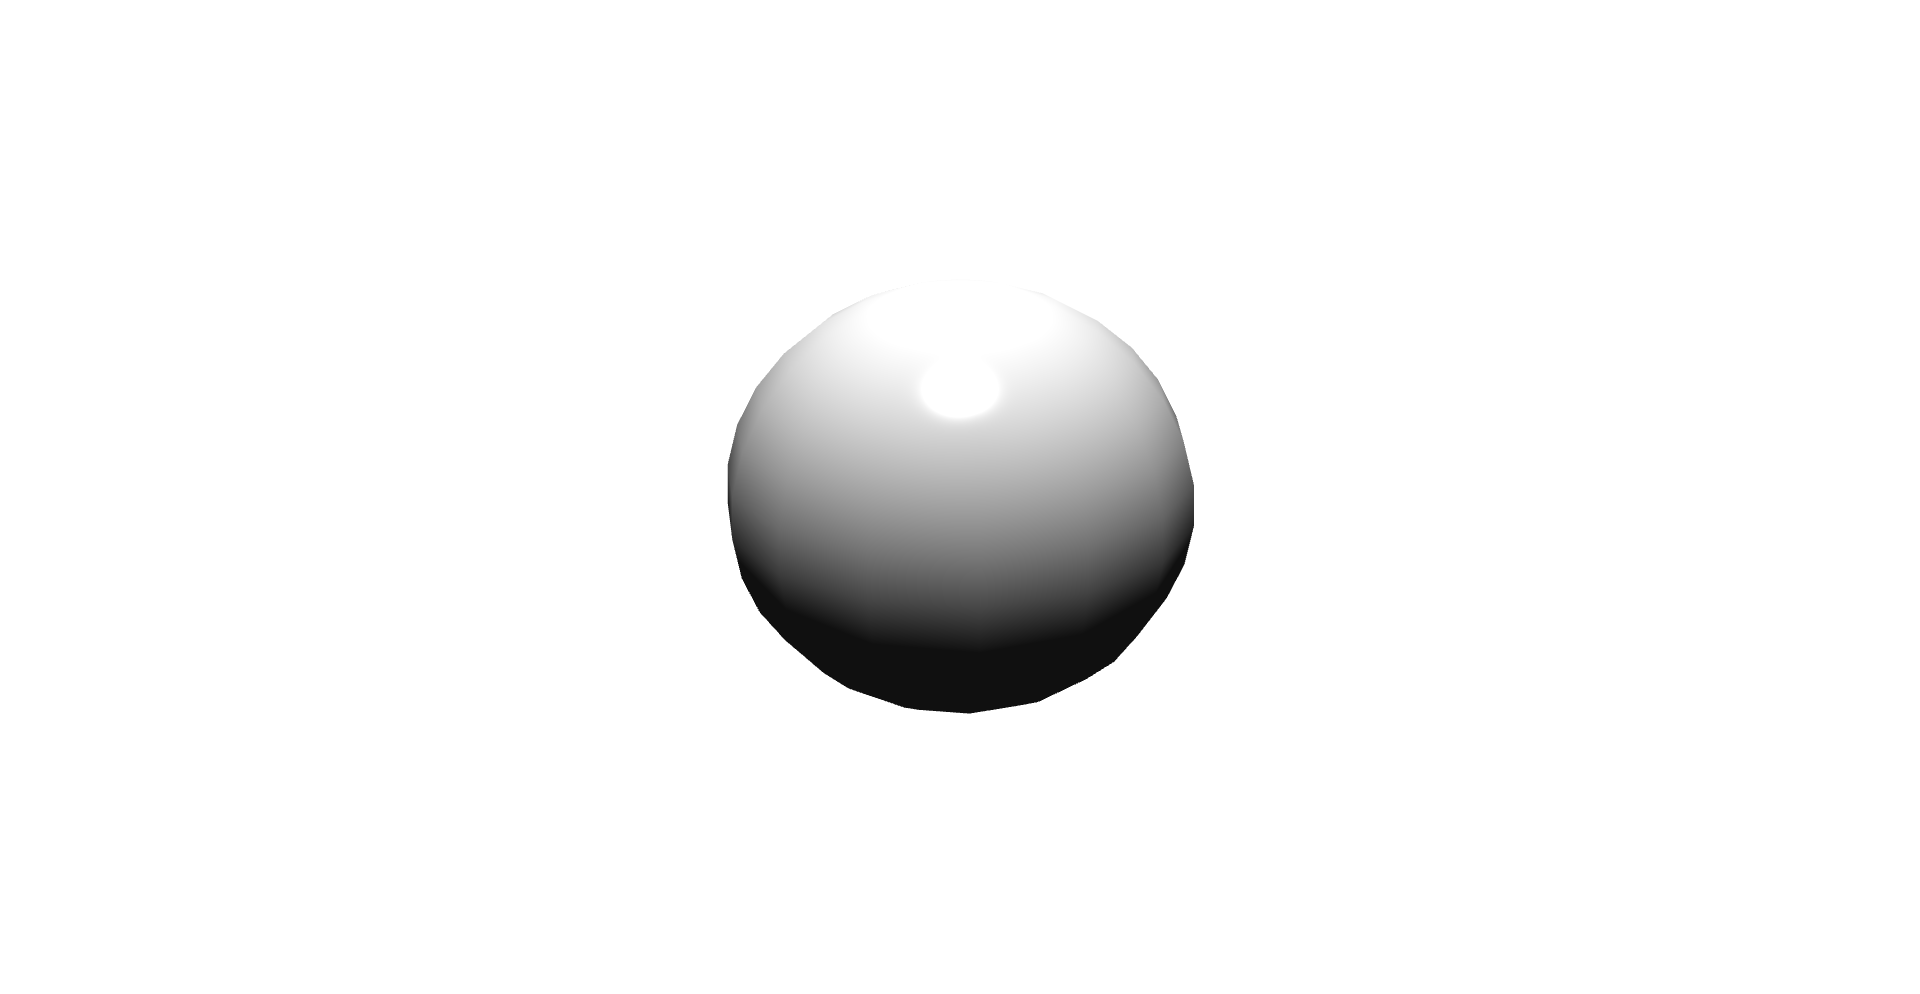
\includegraphics[width=1\linewidth]{sphere/ourPhongSphere.png}}
        \caption{Phong shaded sphere using our implementation.}
        \label{fig:our-phong-sphere}
    \end{subfigure}
    \hfill
    \begin{subfigure}{.48\linewidth}
        \frame{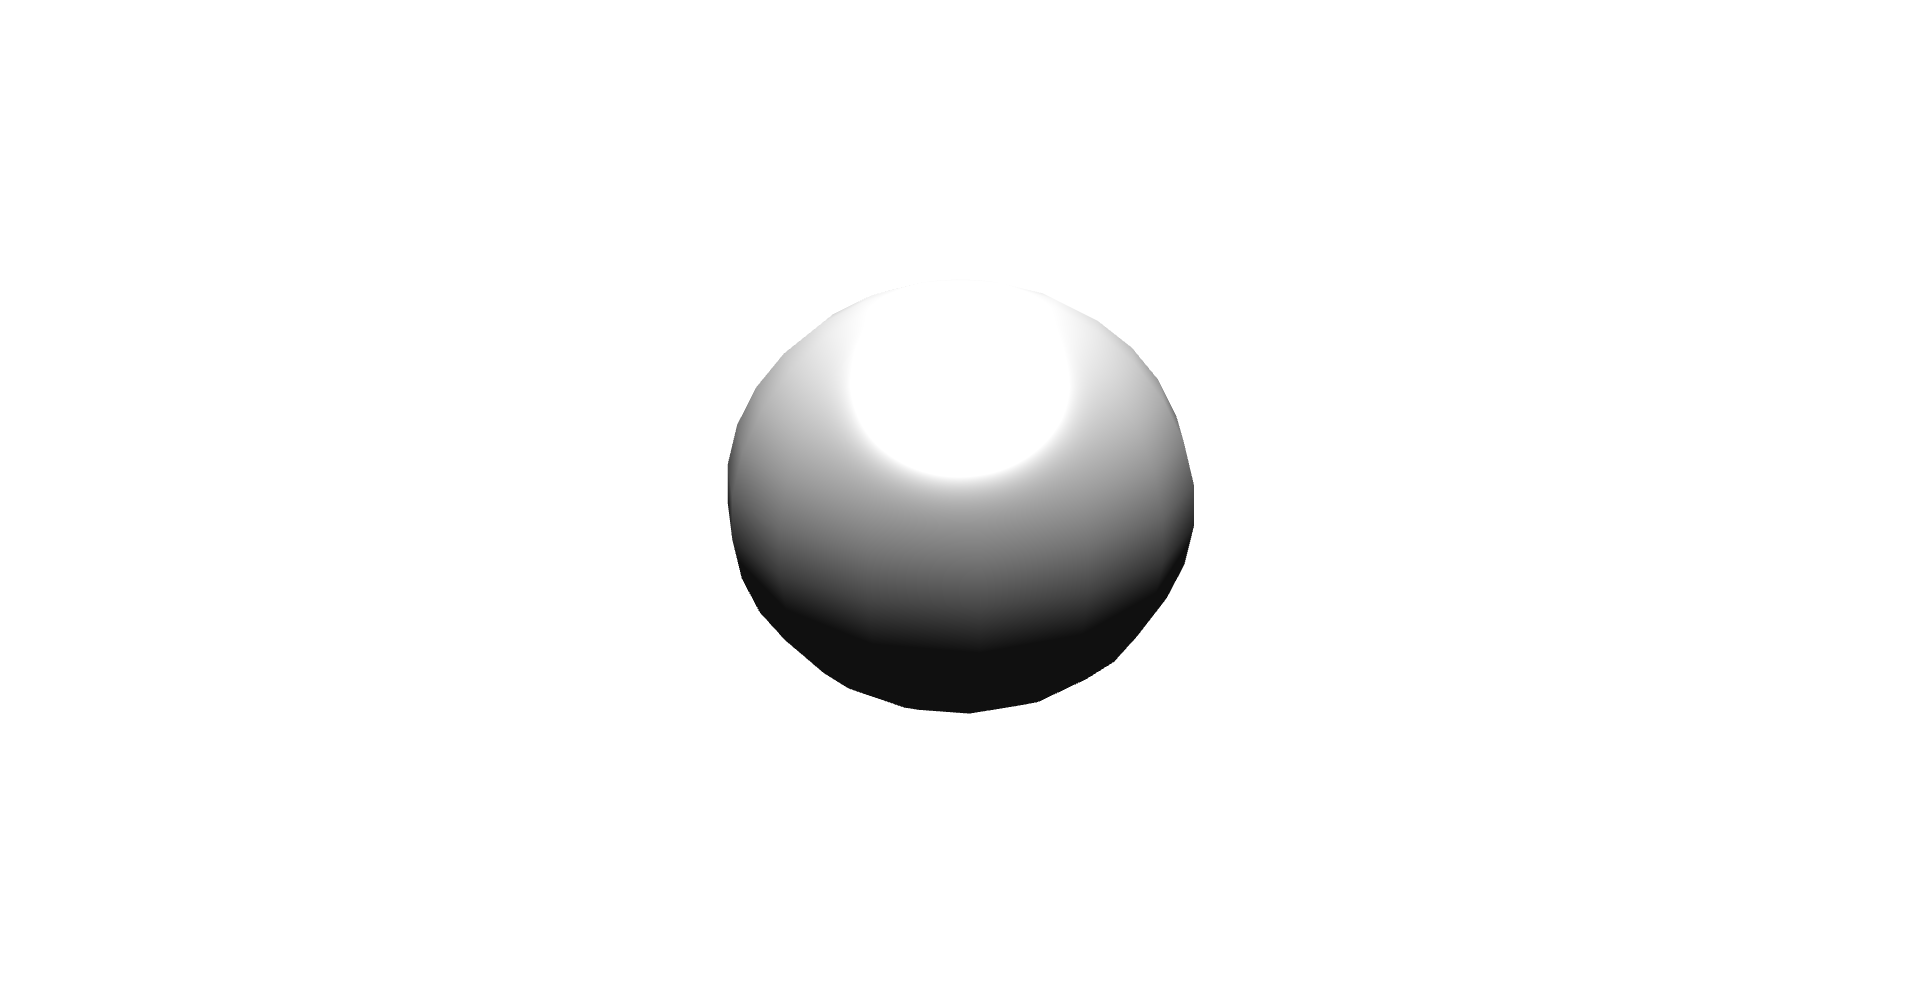
\includegraphics[width=1\linewidth]{sphere/threePhongSphere.png}}
        \caption{Phong shaded sphere using ThreeJS implementation.}
        \label{fig:three-phong-sphere}
    \end{subfigure}
    \caption{Example of Phong shading on a basic sphere mesh, using both Phong normals and Phong lighting. With both specular and ambient light added to the diffuse light calculated from Lambert techniques, the sphere now appears as if it had a "shine." While we did not exactly mimic the way in which the sphere "shines" the way it does in the ThreeJS implementation, we decided that our implementation had a good enough accent of light, which already achieves the purpose of Phong shading.}
    \label{fig:phong-sphere}
\end{figure*}

%--Torus Knot--

\begin{figure*}
    \centering
    \begin{subfigure}{.48\linewidth}
        \frame{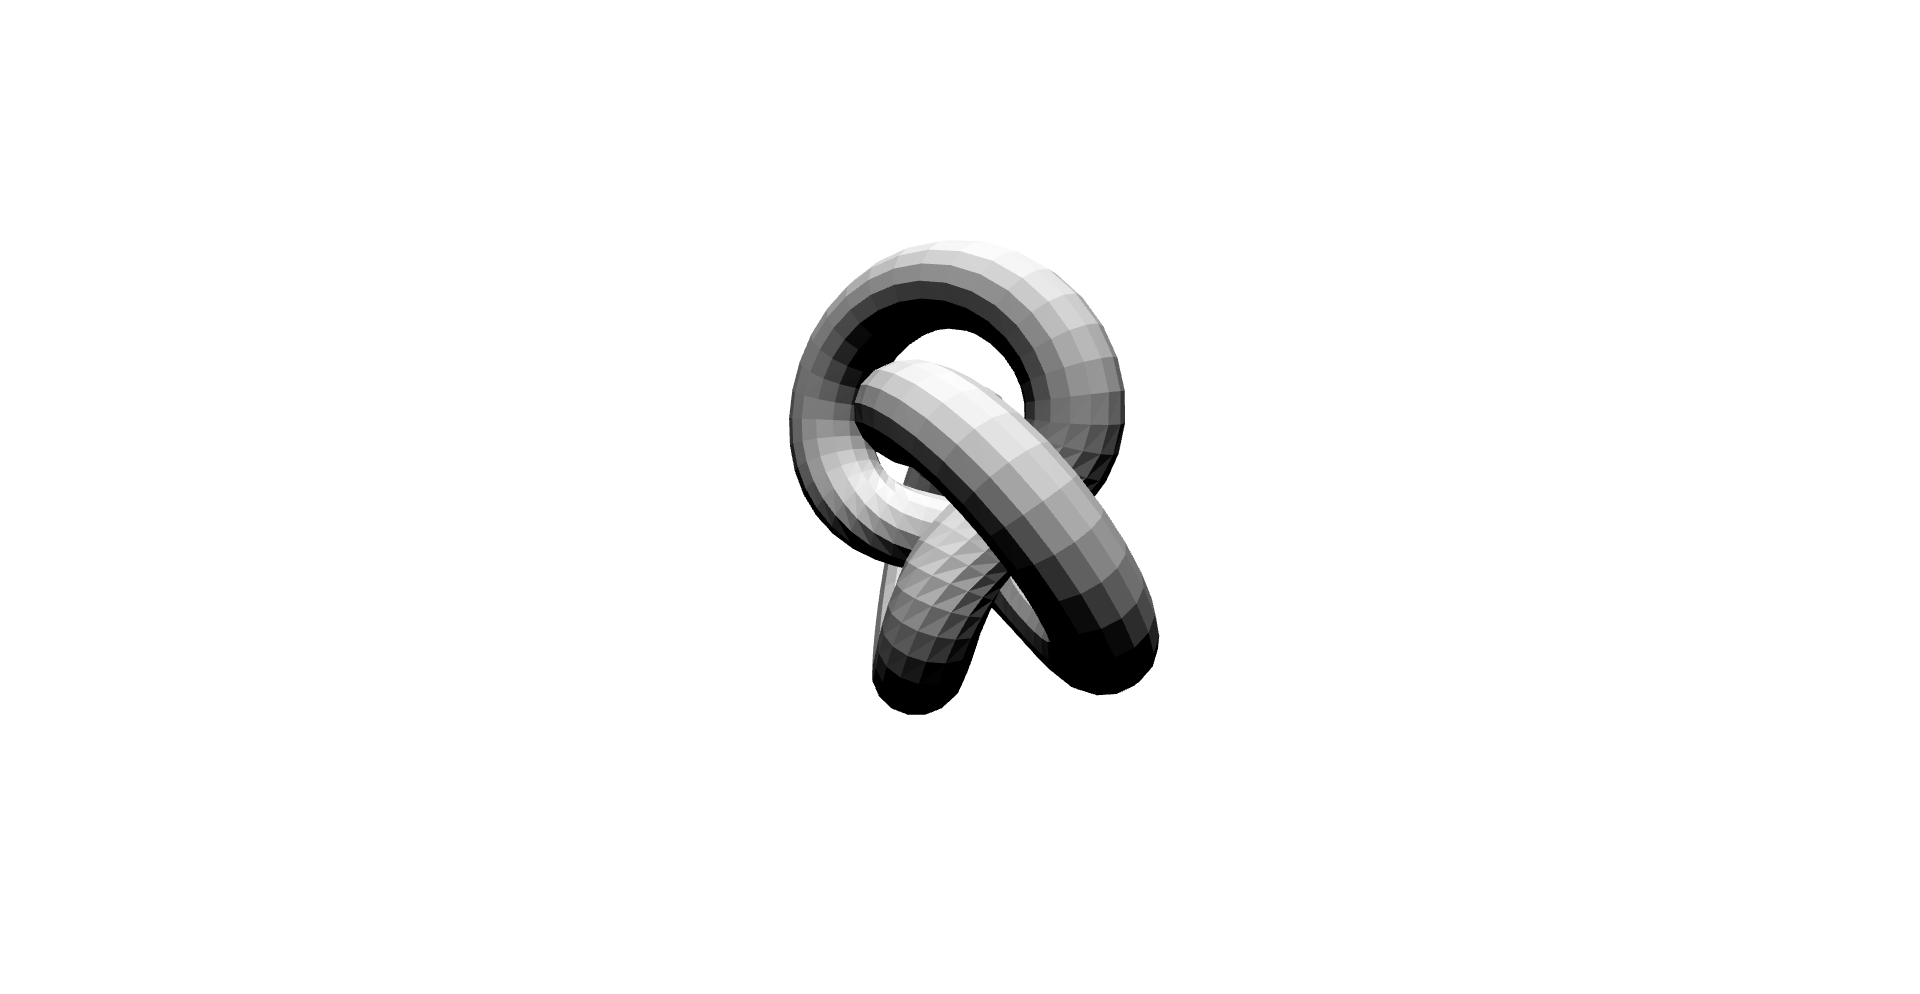
\includegraphics[width=1\linewidth]{torusKnot/ourFlatTK.png}}
        \caption{Flat shaded torus knot using our implementation.}
        \label{fig:our-flat-tk}
    \end{subfigure}
    \hfill
    \begin{subfigure}{.48\linewidth}
        \frame{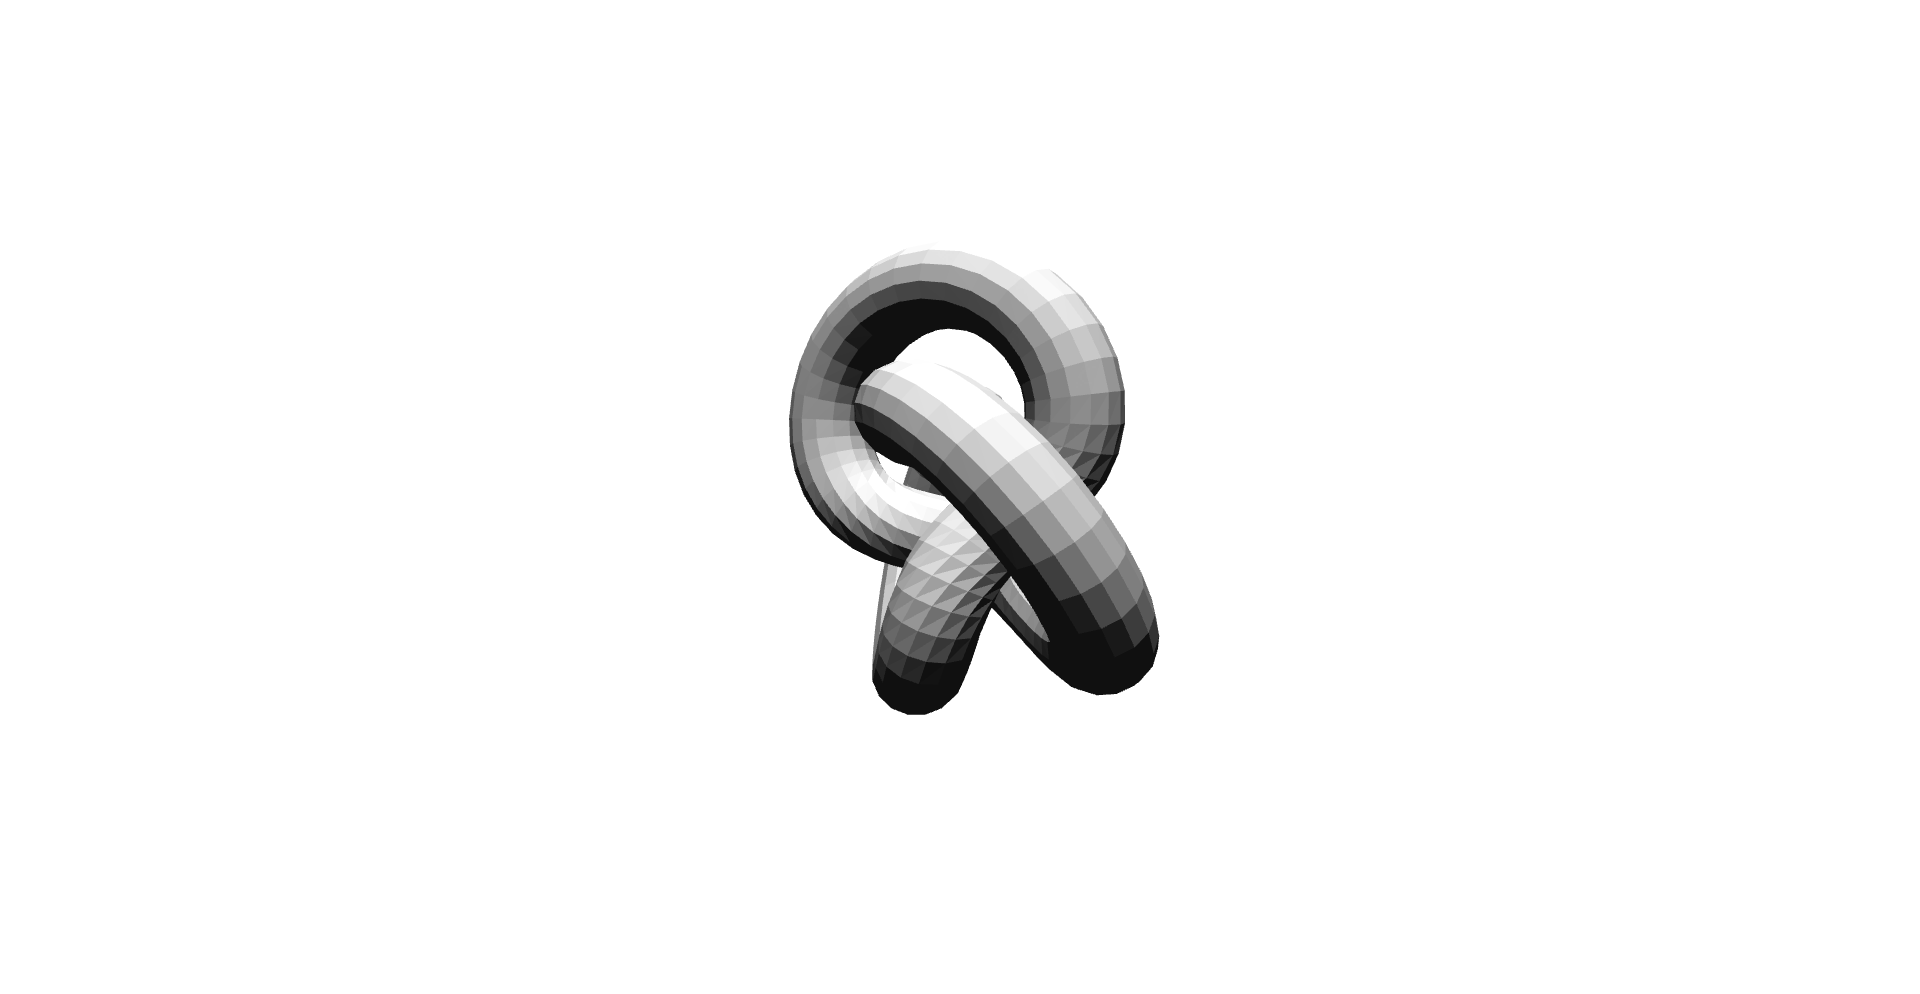
\includegraphics[width=1\linewidth]{torusKnot/threeFlatTK.png}}
        \caption{Flat shaded torus knot using ThreeJS implementation.}
        \label{fig:three-flat-tk}
    \end{subfigure}
    \caption{Example of Flat shading on a basic torus knot mesh. Again, the faces of the mesh are more apparent under flat shading.}
    \label{fig:flat-tk}
\end{figure*}

\begin{figure*}
    \centering
    \begin{subfigure}{.48\linewidth}
        \frame{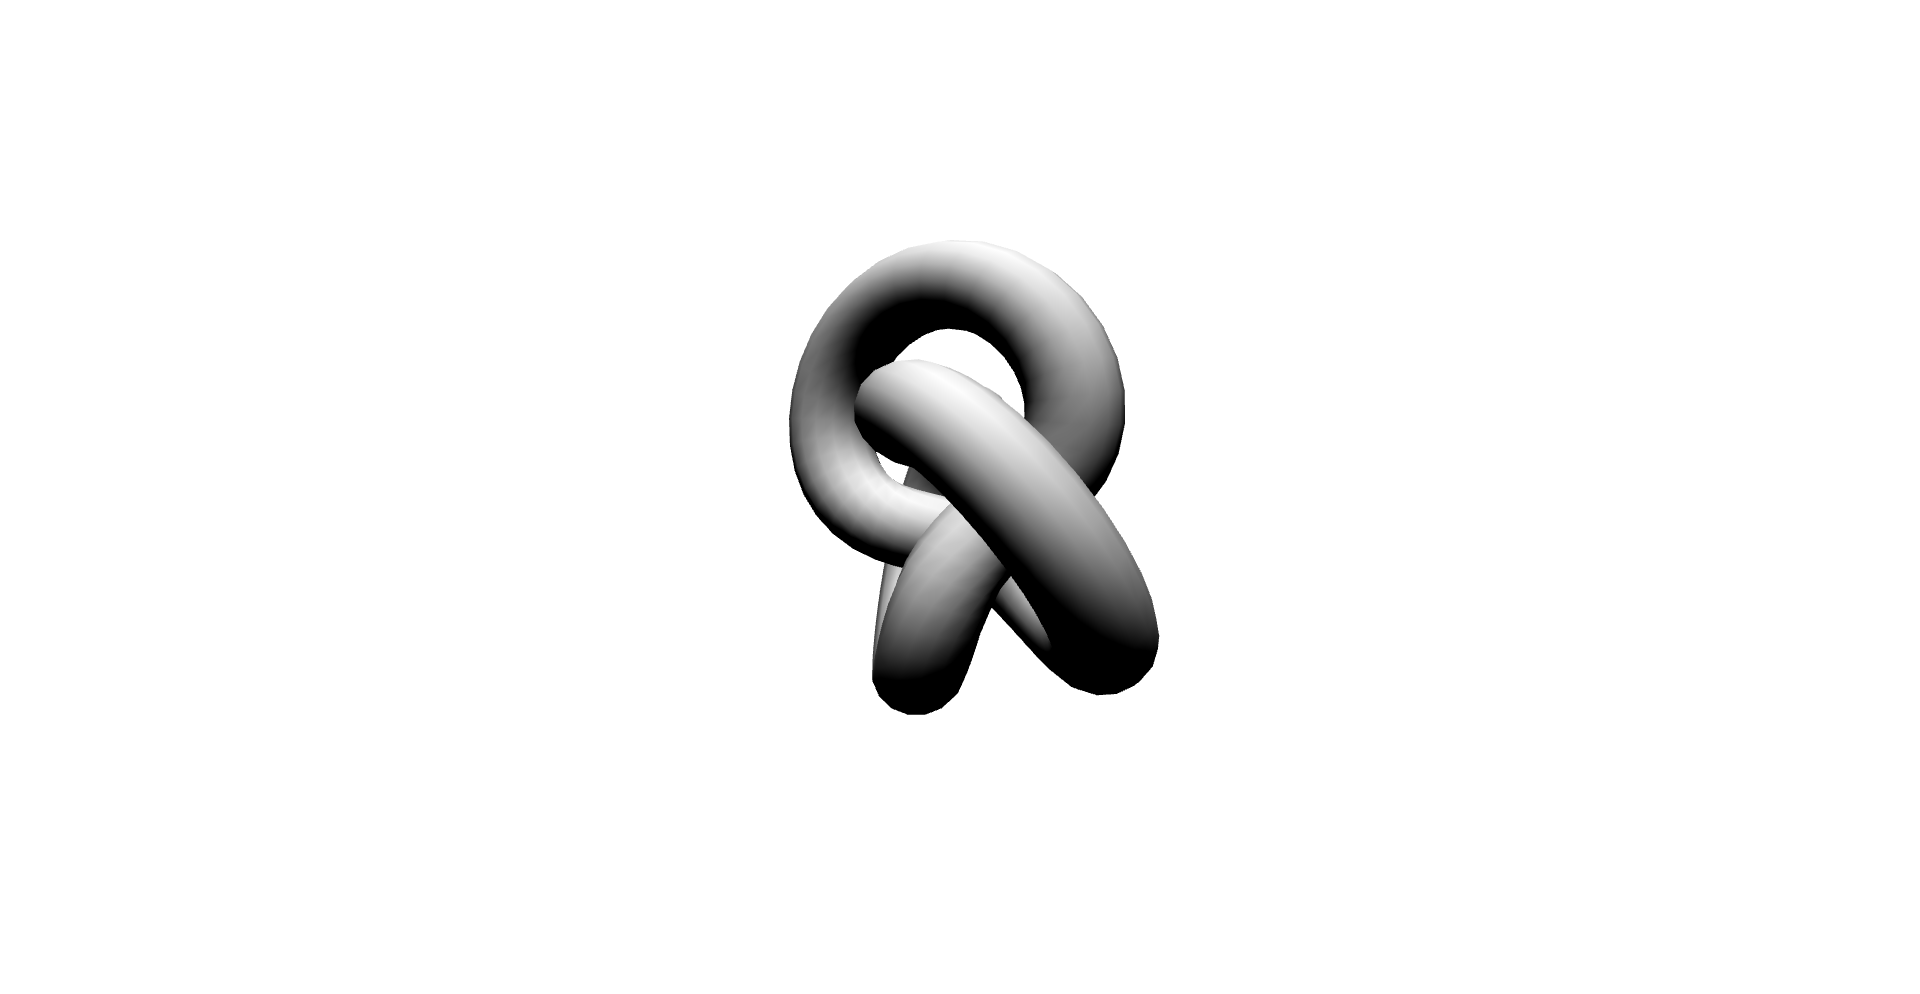
\includegraphics[width=1\linewidth]{torusKnot/ourGouraudTK.png}}
        \caption{Gouraud shaded torus knot using our implementation.}
        \label{fig:our-gouraud-tk}
    \end{subfigure}
    \hfill
    \begin{subfigure}{.48\linewidth}
        \frame{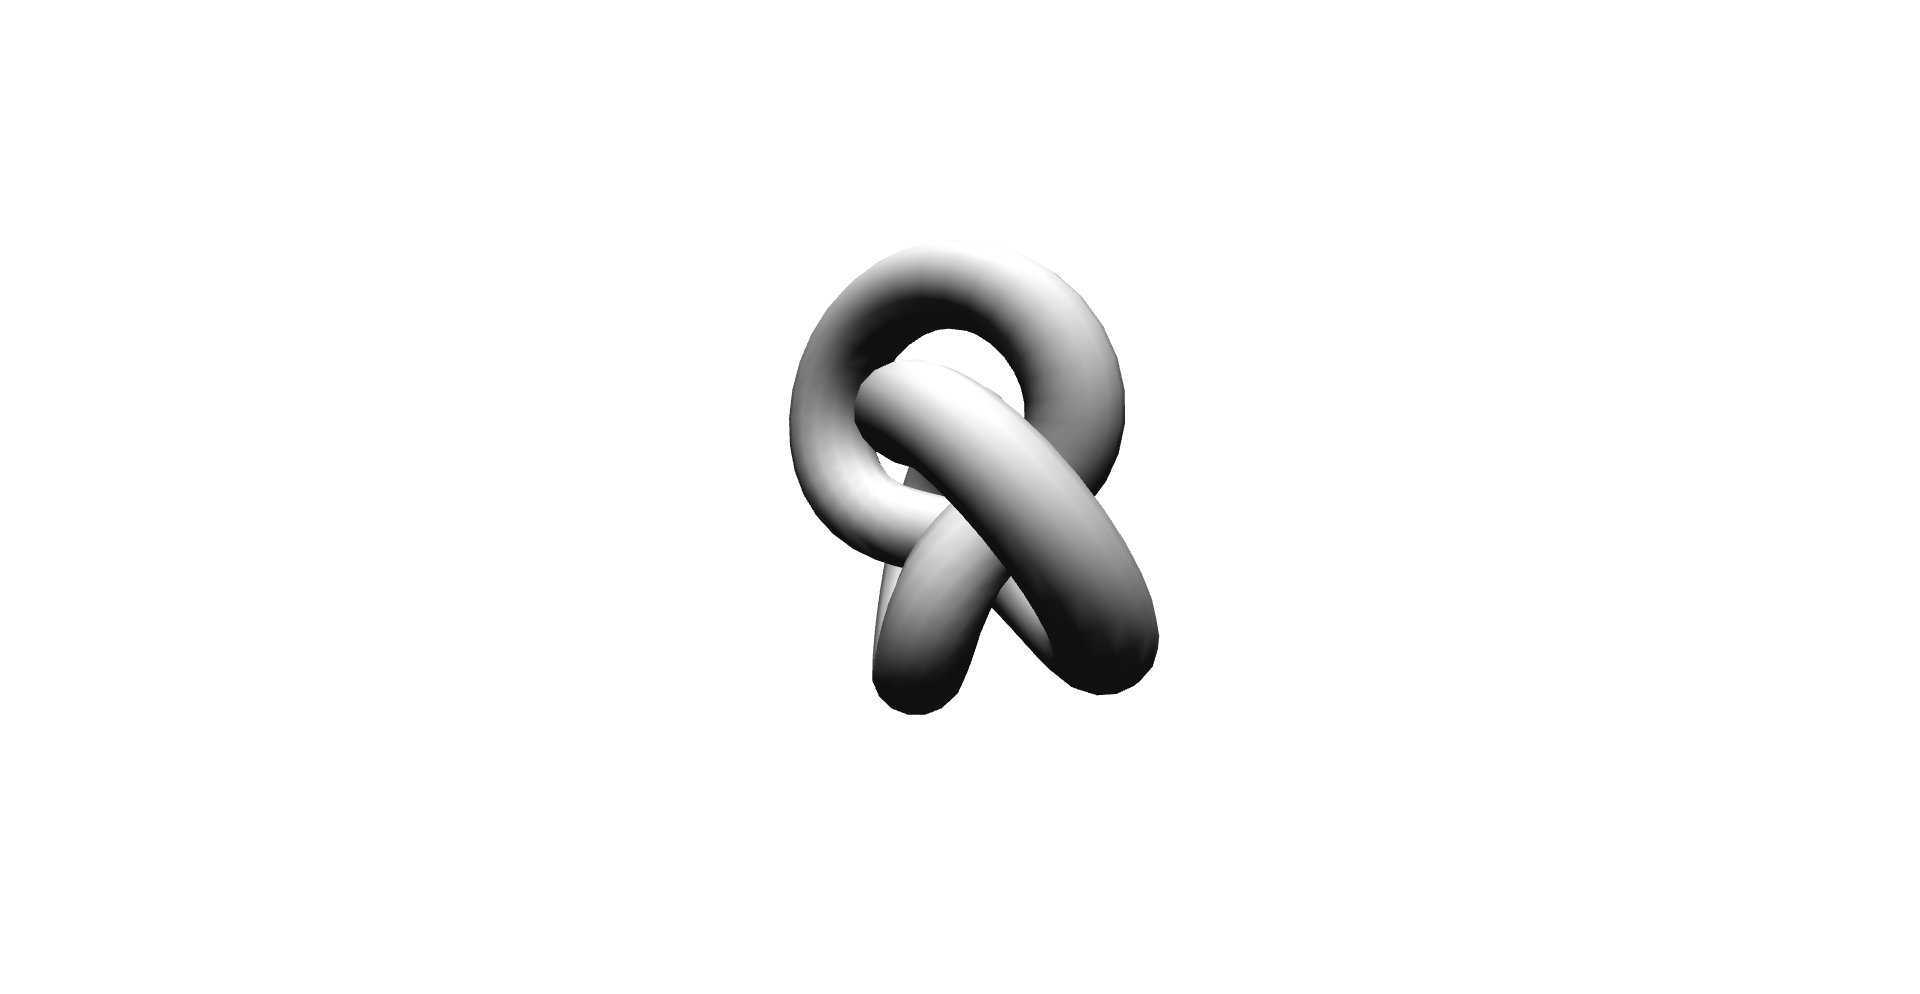
\includegraphics[width=1\linewidth]{torusKnot/threeGouraudTK.png}}
        \caption{Gouraud shaded torus knot using ThreeJS implementation.}
        \label{fig:three-gouraud-tk}
    \end{subfigure}
    \caption{Example of Gouraud shading on a basic torus knot mesh. Again, the edges of the mesh are more differentiable from the rest of the surface.}
    \label{fig:gouraud-tk}
\end{figure*}

\begin{figure*}
    \centering
    \begin{subfigure}{.48\linewidth}
        \frame{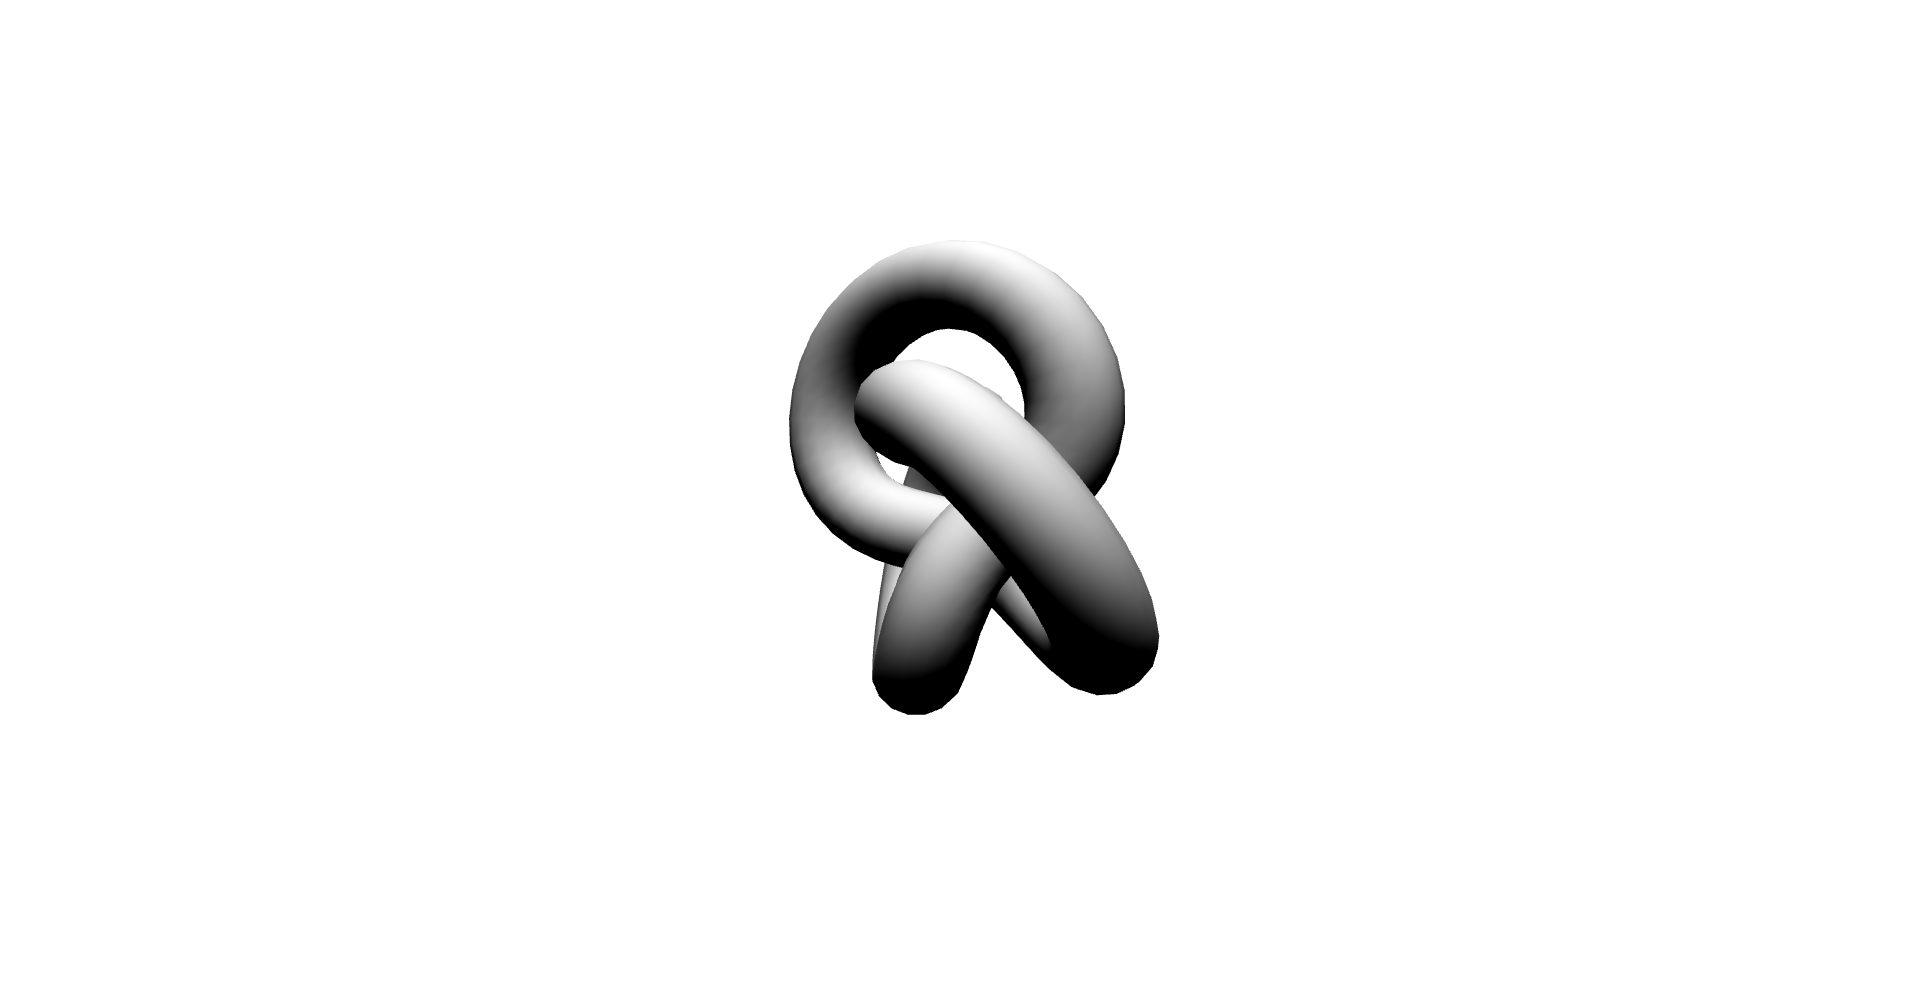
\includegraphics[width=1\linewidth]{torusKnot/ourLambertTK.png}}
        \caption{Lambert shaded torus knot using our implementation.}
        \label{fig:our-lambert-tk}
    \end{subfigure}
    \hfill
    \begin{subfigure}{.48\linewidth}
        \frame{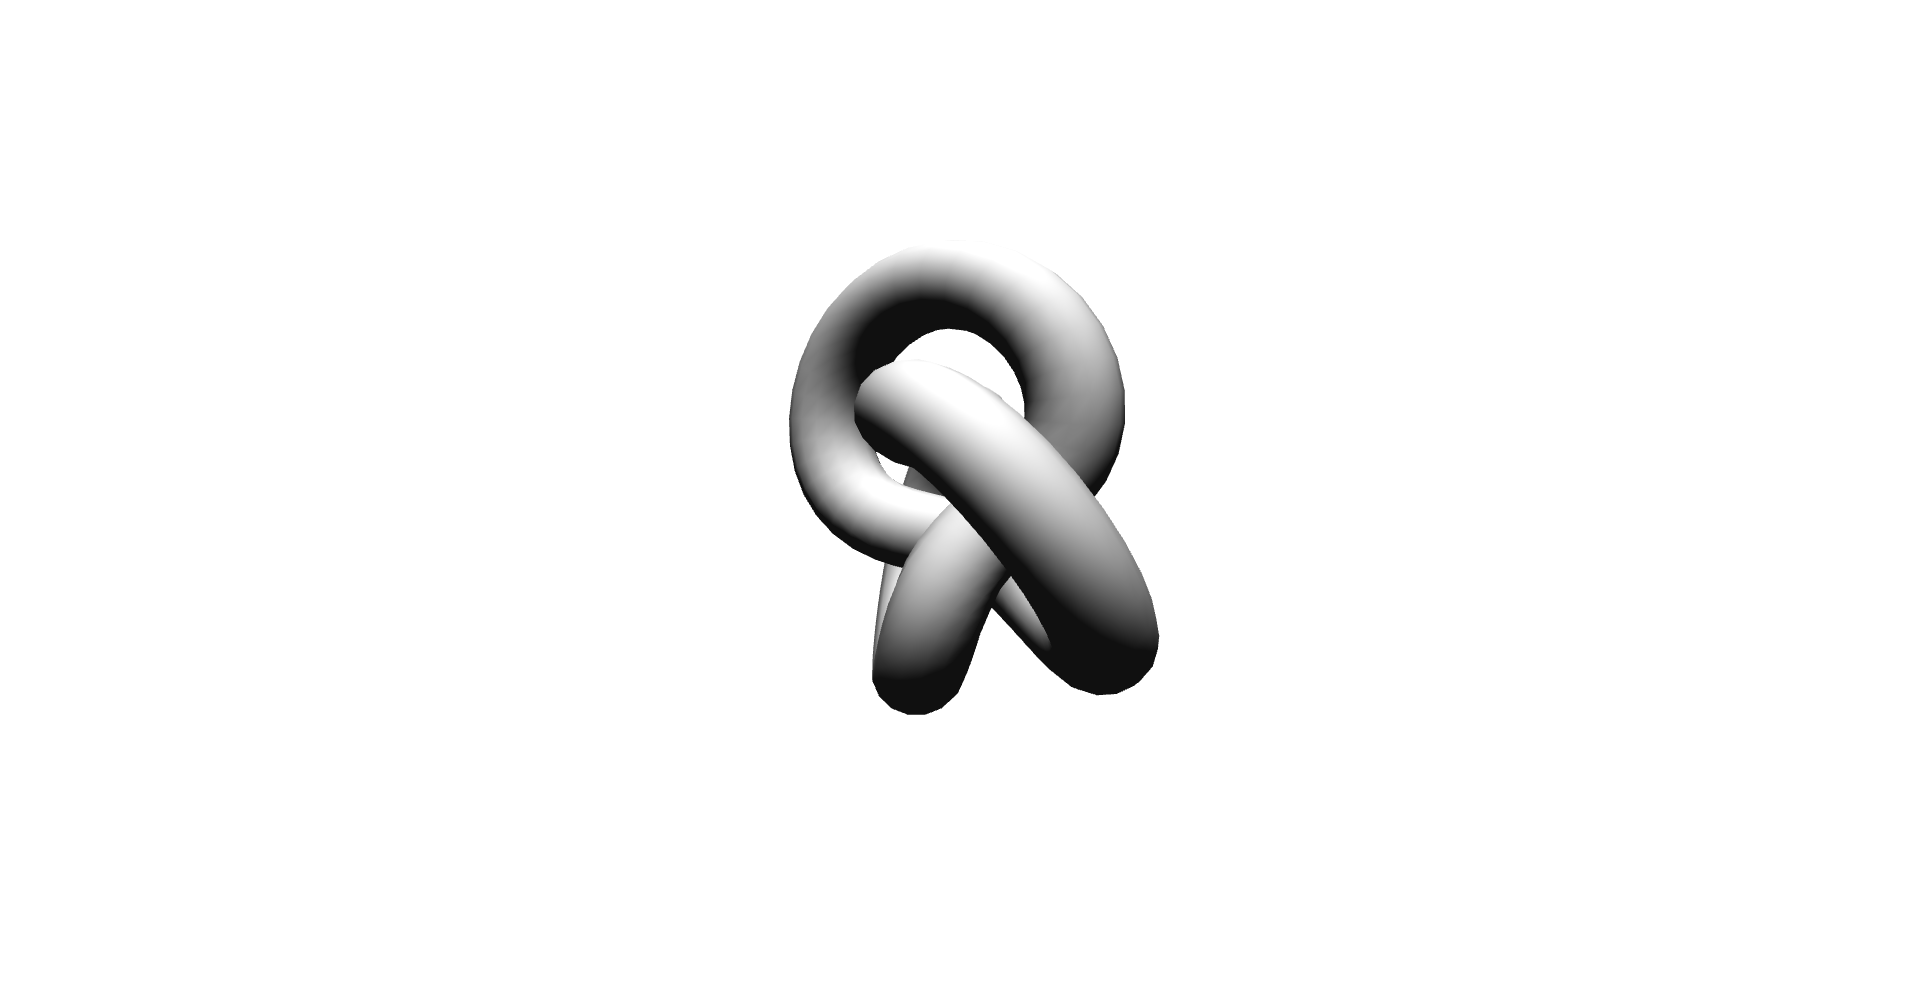
\includegraphics[width=1\linewidth]{torusKnot/threeLambertTK.png}}
        \caption{Lambert shaded torus knot using ThreeJS implementation.}
        \label{fig:three-lambert-tk}
    \end{subfigure}
    \caption{Example of Lambert shading on a basic torus knot mesh with Phong normals. Again, the interpolated normals in the shader gives the shape an "smoother" appearence.}
    \label{fig:lambert-tk}
\end{figure*}

\begin{figure*}
    \centering
    \begin{subfigure}{.48\linewidth}
        \frame{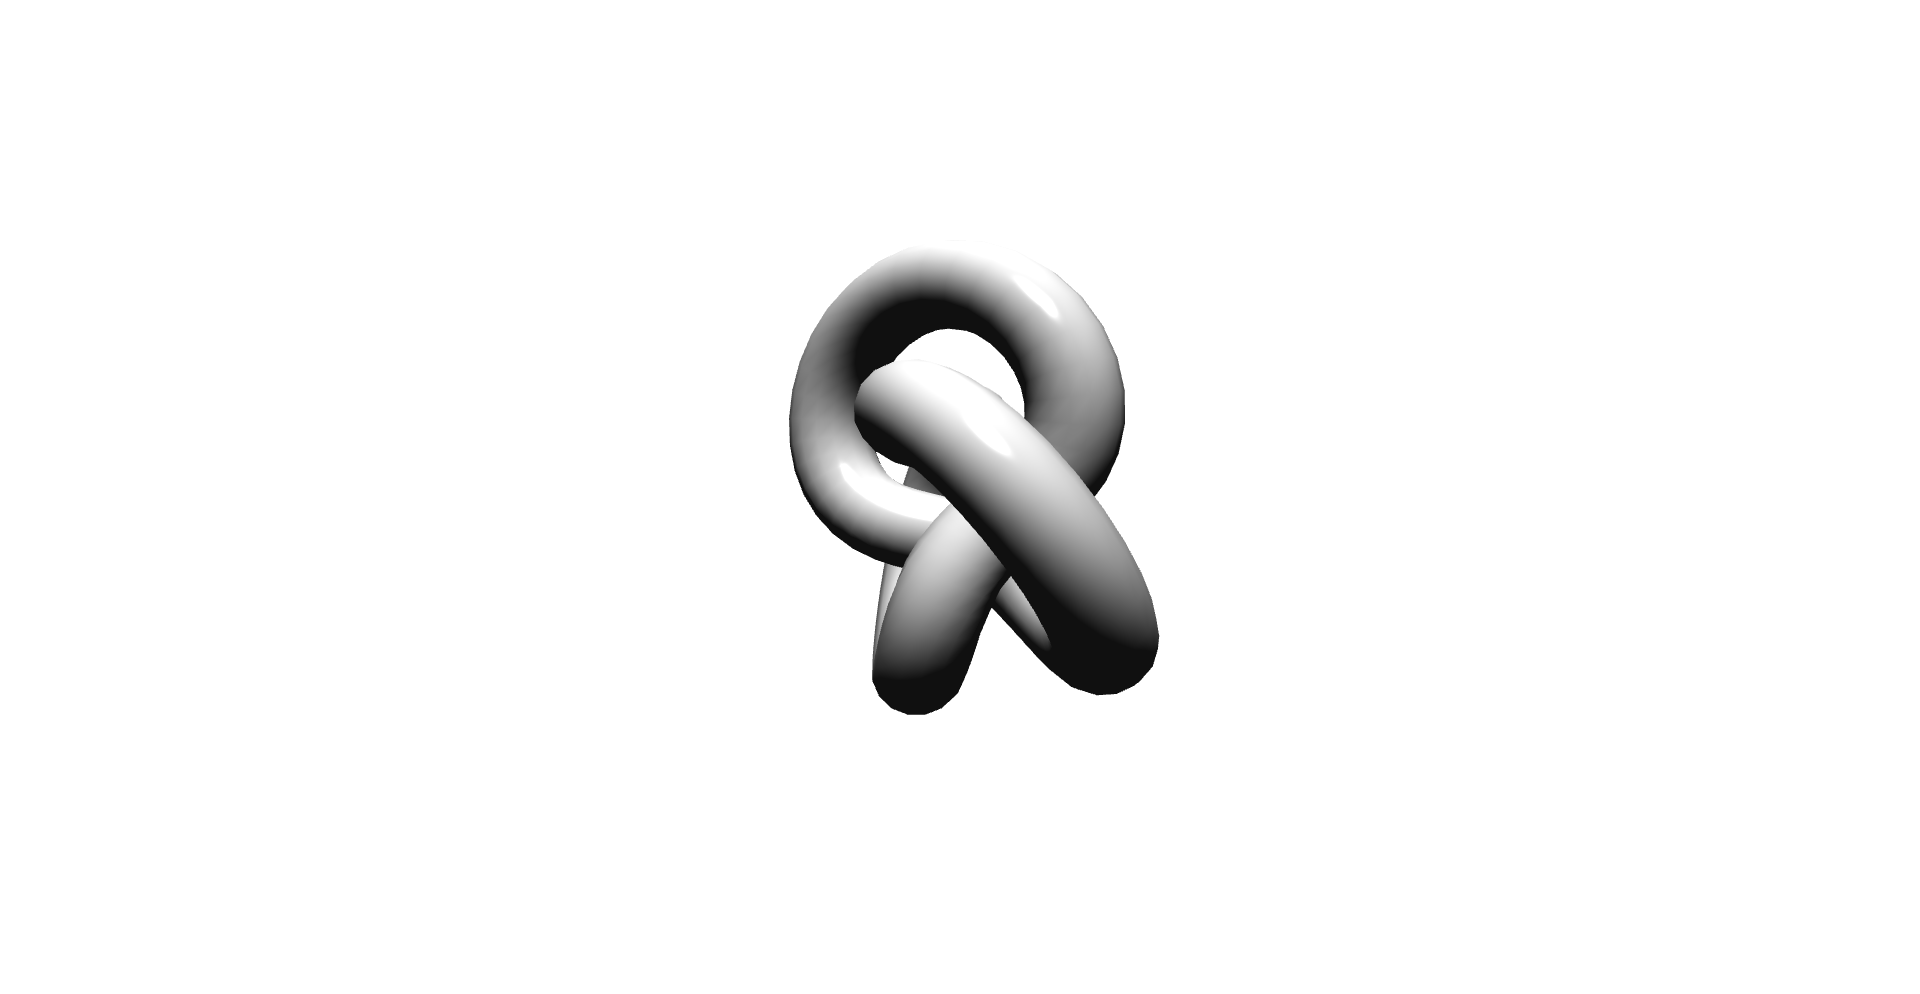
\includegraphics[width=1\linewidth]{torusKnot/ourPhongTK.png}}
        \caption{Phong shaded torus knot using our implementation.}
        \label{fig:our-phong-tk}
    \end{subfigure}
    \hfill
    \begin{subfigure}{.48\linewidth}
        \frame{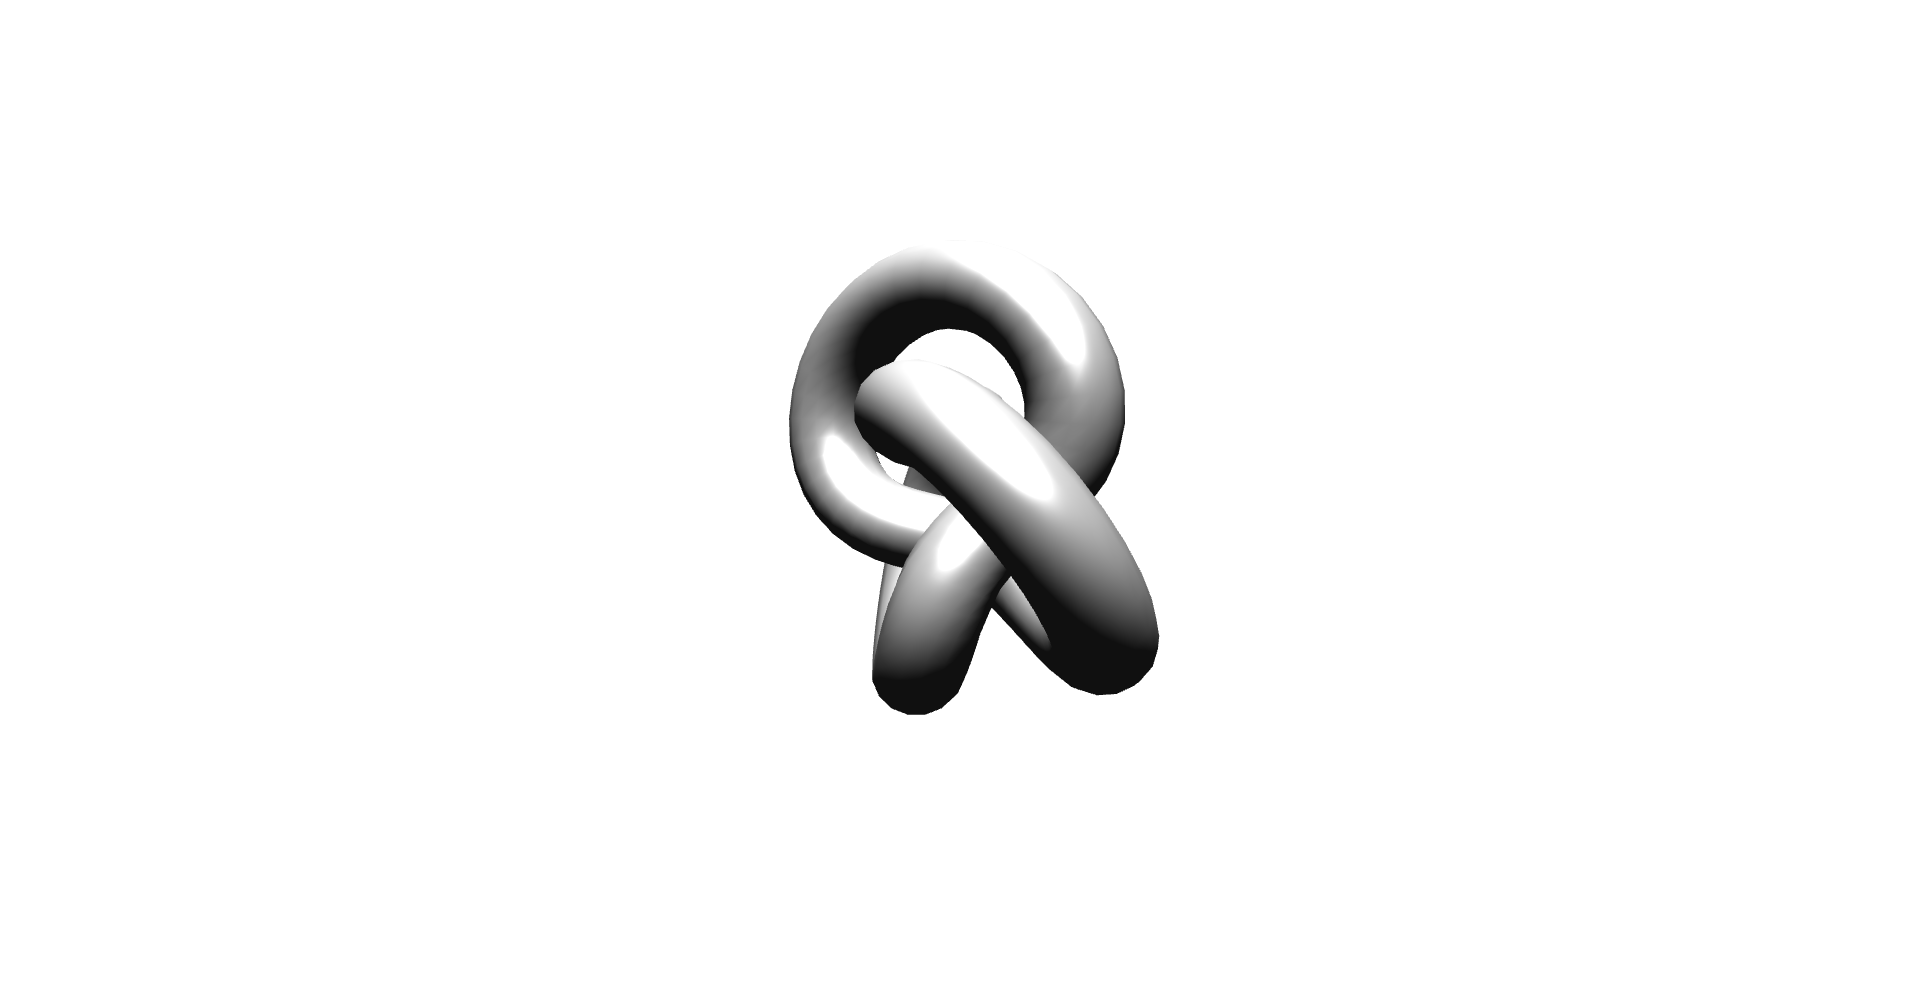
\includegraphics[width=1\linewidth]{torusKnot/threePhongTK.png}}
        \caption{Phong shaded torus knot using ThreeJS implementation.}
        \label{fig:three-phong-tk}
    \end{subfigure}
    \caption{Example of Phong shading on a basic torus knot mesh, using both Phong normals and Phong lighting. Again, the added layers of light gives the shape a "shinier" appearence.}
    \label{fig:phong-tk}
\end{figure*}

%--Utah Teapot--

\begin{figure*}
    \centering
    \begin{subfigure}{.48\linewidth}
        \frame{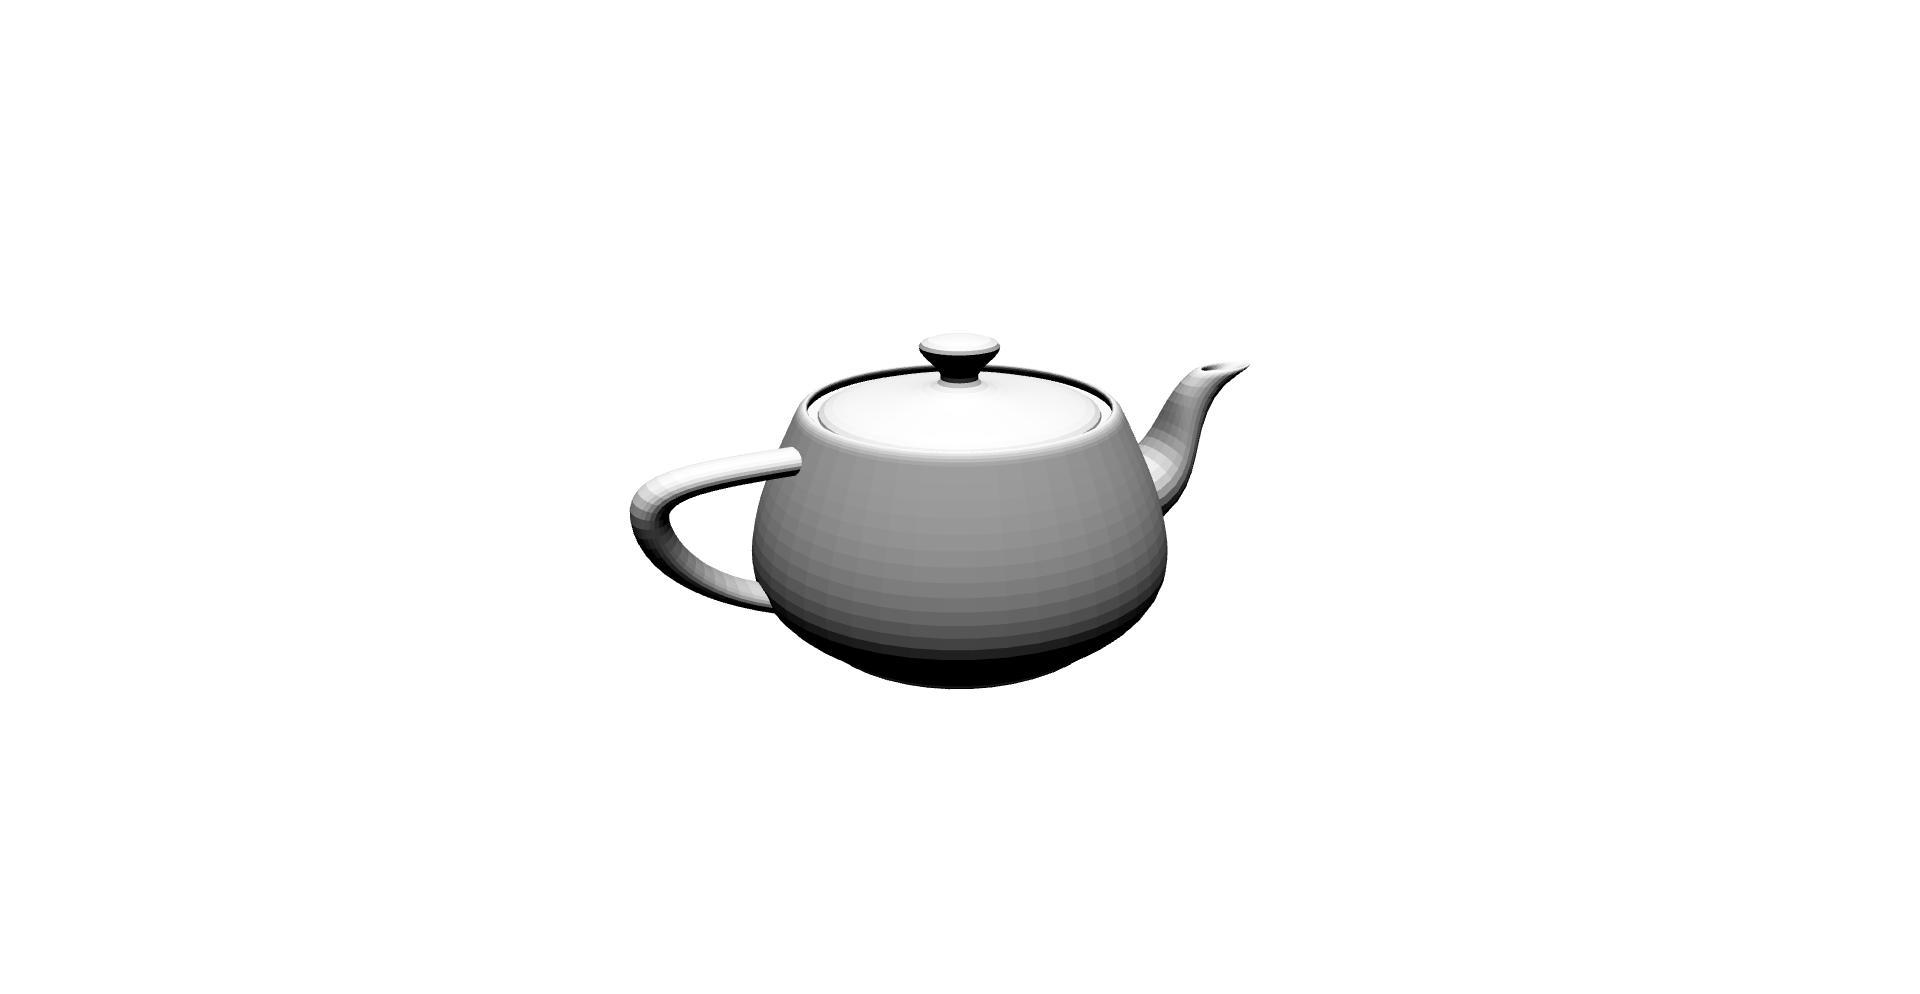
\includegraphics[width=1\linewidth]{teapot/ourFlatTea.png}}
        \caption{Flat shaded teapot using our implementation.}
        \label{fig:our-flat-tea}
    \end{subfigure}
    \hfill
    \begin{subfigure}{.48\linewidth}
        \frame{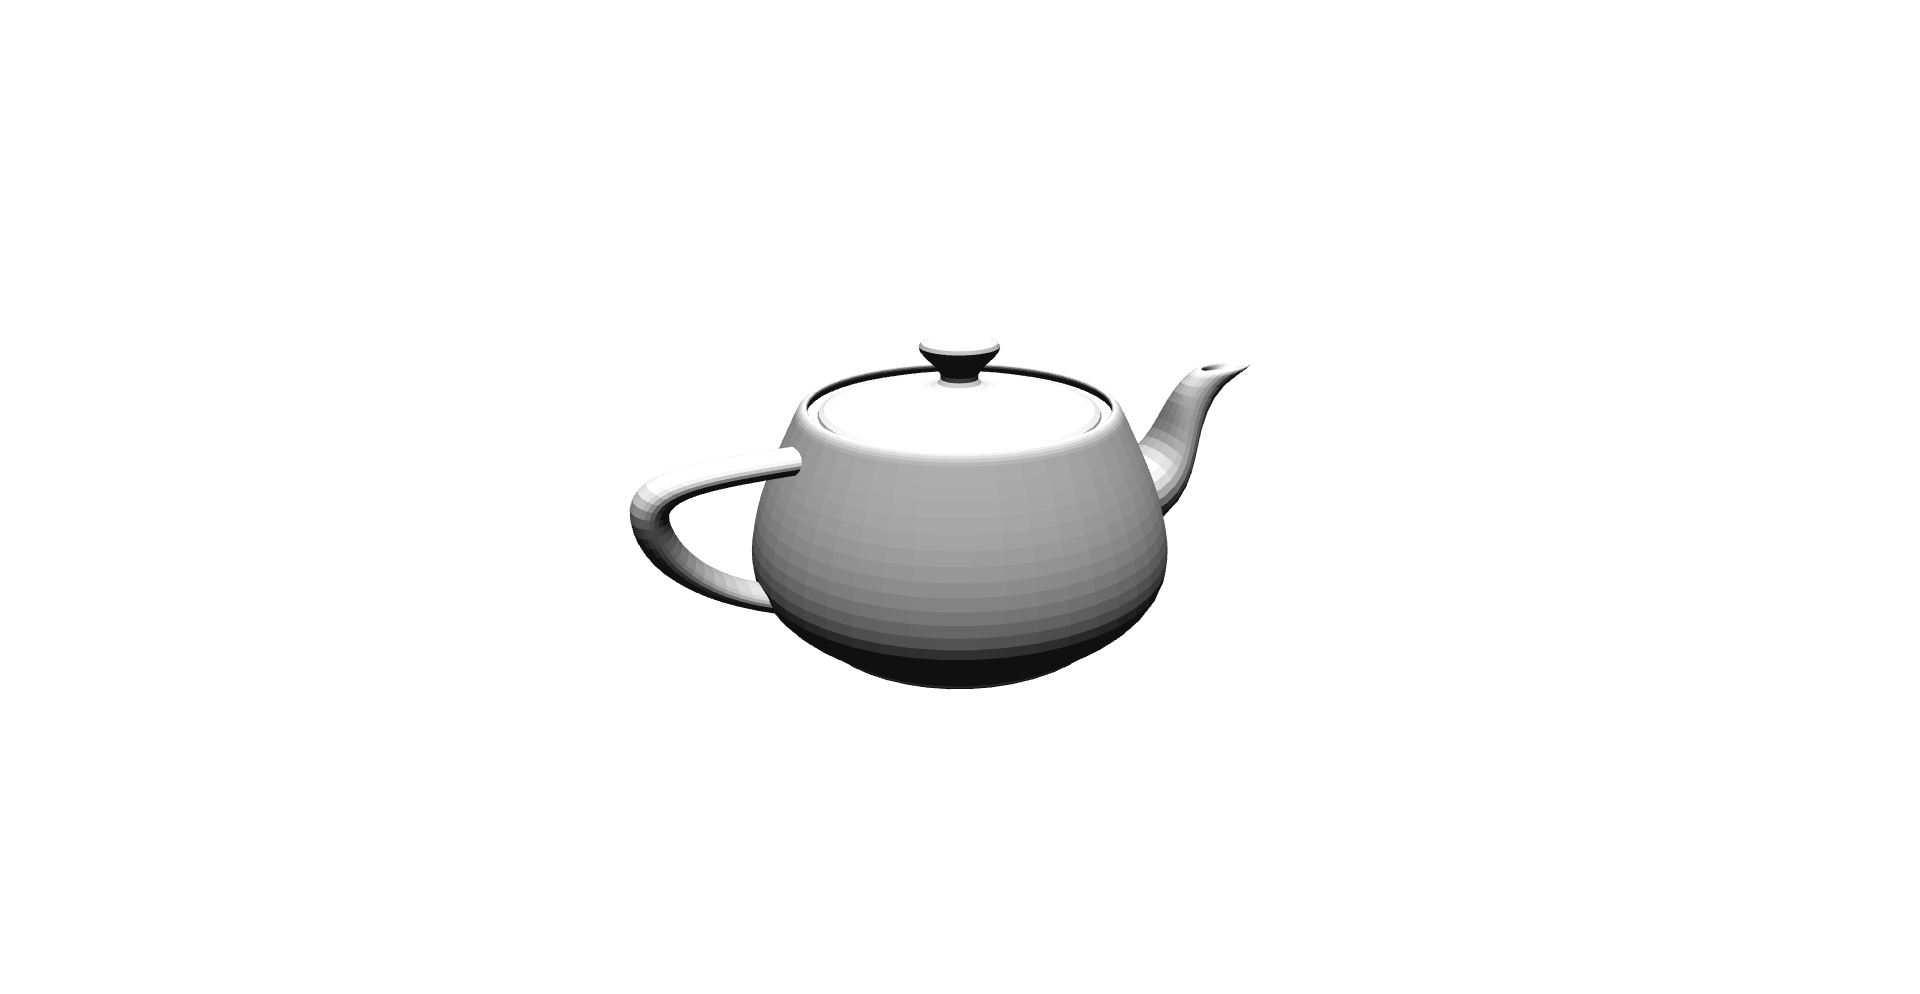
\includegraphics[width=1\linewidth]{teapot/threeFlatTea.png}}
        \caption{Flat shaded teapot using ThreeJS implementation.}
        \label{fig:three-flat-tea}
    \end{subfigure}
    \caption{Example of Flat shading on the Utah Teapot mesh. Since this particular mesh has more polygons, the result shows a lot more faces, allowing the final rendering to appear more round.}
    \label{fig:flat-tea}
\end{figure*}

\begin{figure*}
    \centering
    \begin{subfigure}{.48\linewidth}
        \frame{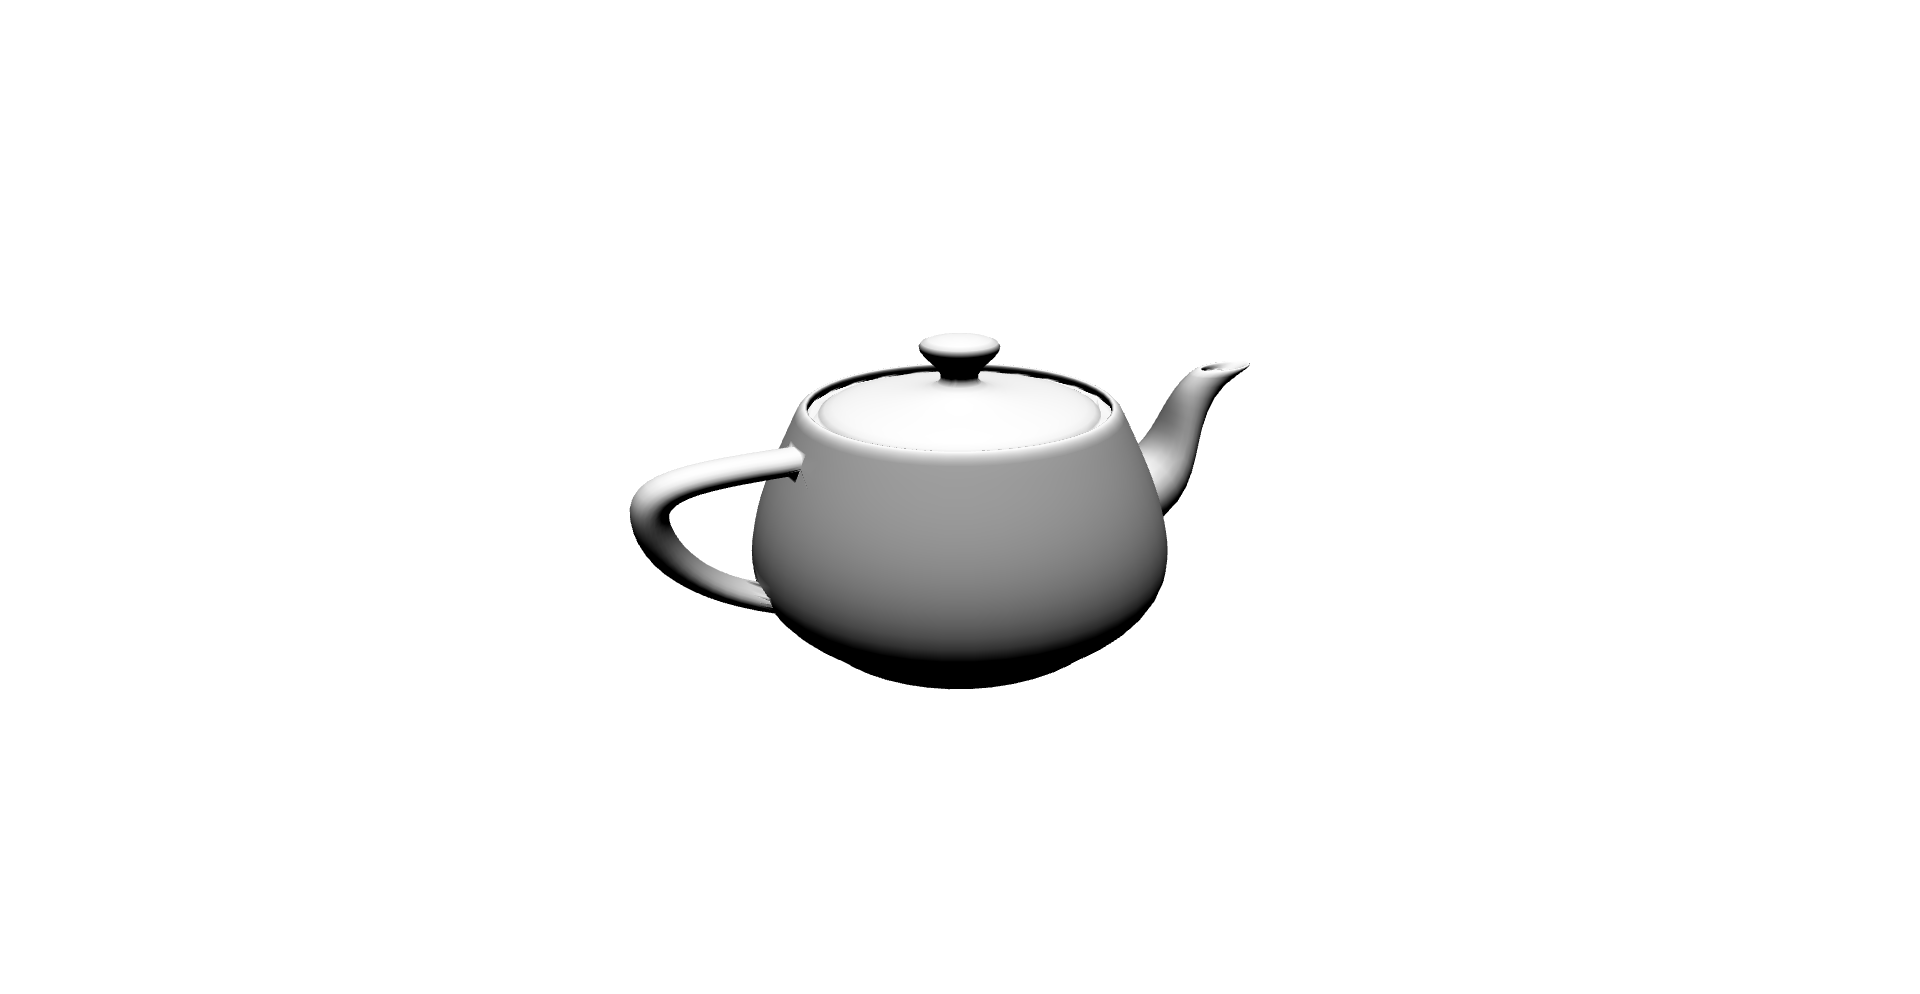
\includegraphics[width=1\linewidth]{teapot/ourGouraudTea.png}}
        \caption{Gouraud shaded teapot using our implementation.}
        \label{fig:our-gouraud-tea}
    \end{subfigure}
    \hfill
    \begin{subfigure}{.48\linewidth}
        \frame{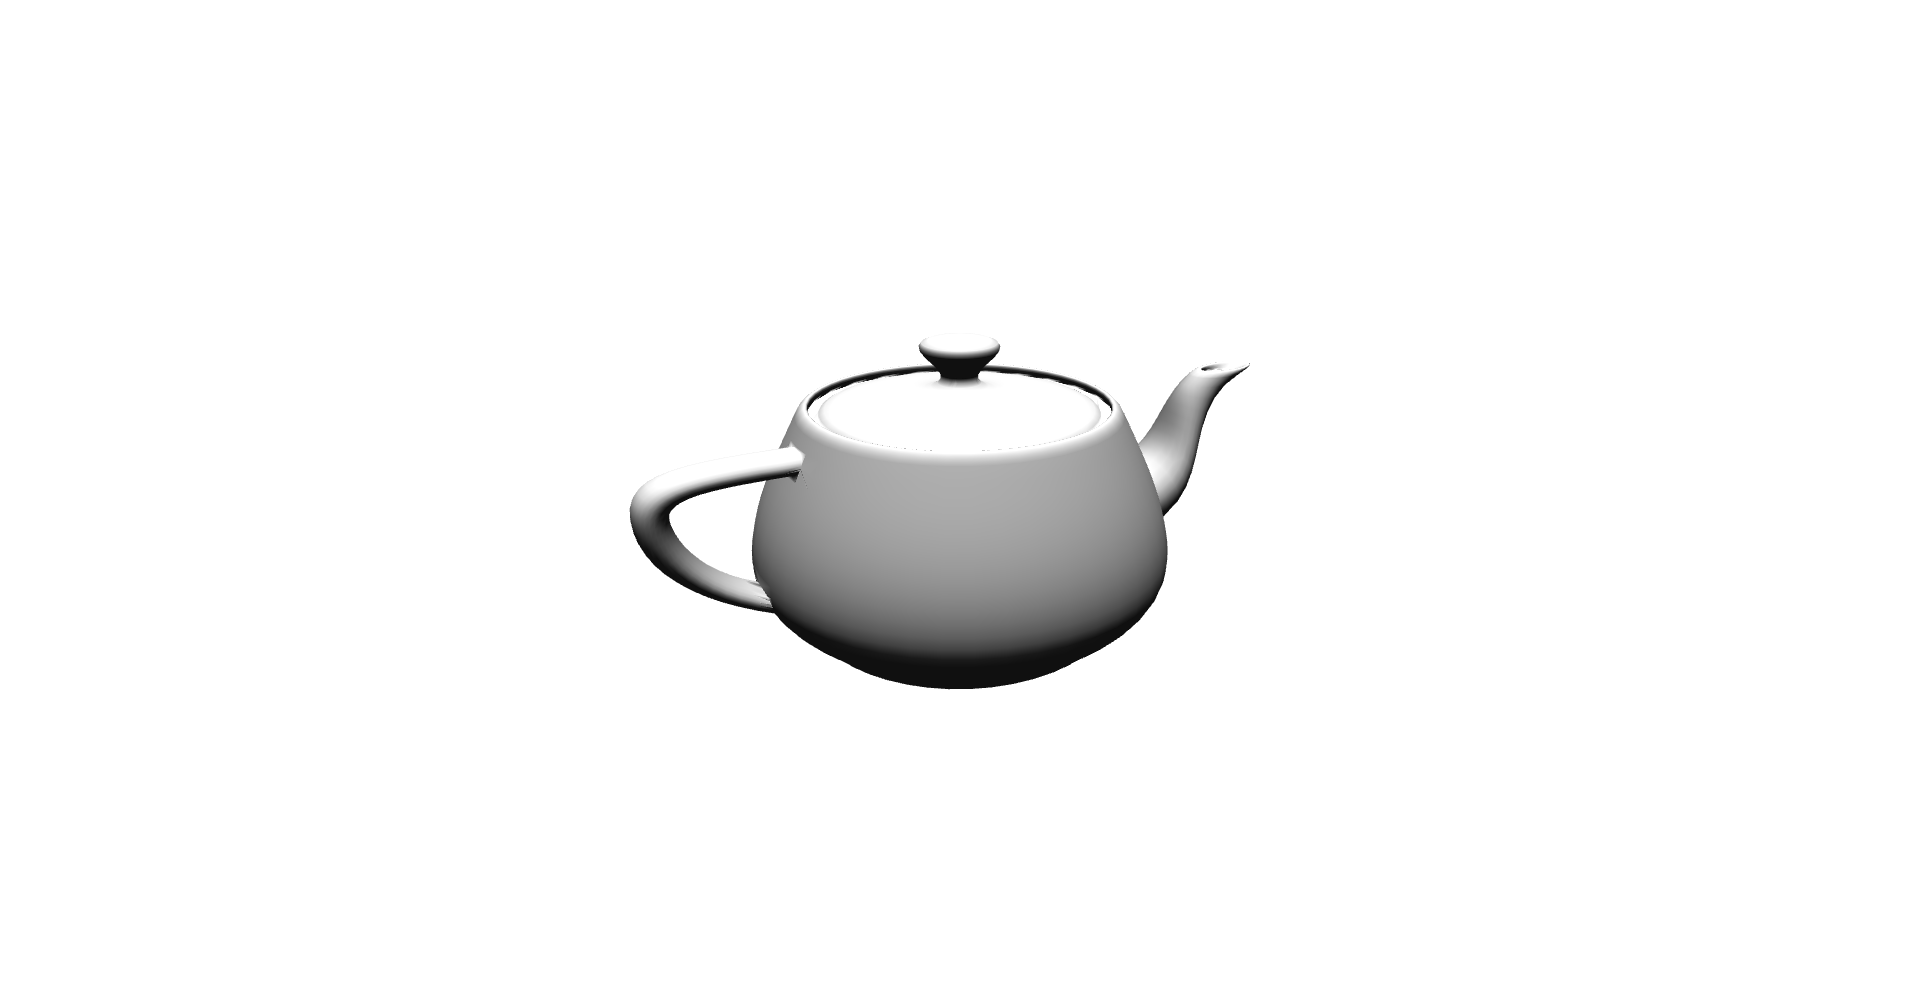
\includegraphics[width=1\linewidth]{teapot/threeGouraudTea.png}}
        \caption{Gouraud shaded teapot using ThreeJS implementation.}
        \label{fig:three-gouraud-tea}
    \end{subfigure}
    \caption{Example of Gouraud shading on the Utah Teapot mesh. Because this mesh has more polygons, edges are shorter and more frequent, allowing their distict color to be barely noticable. This changes the general color of the teapot allowing the main disadvantage of Gouraud shading to be somewhat bypassed.}
    \label{fig:gouraud-tea}
\end{figure*}

\begin{figure*}
    \centering
    \begin{subfigure}{.48\linewidth}
        \frame{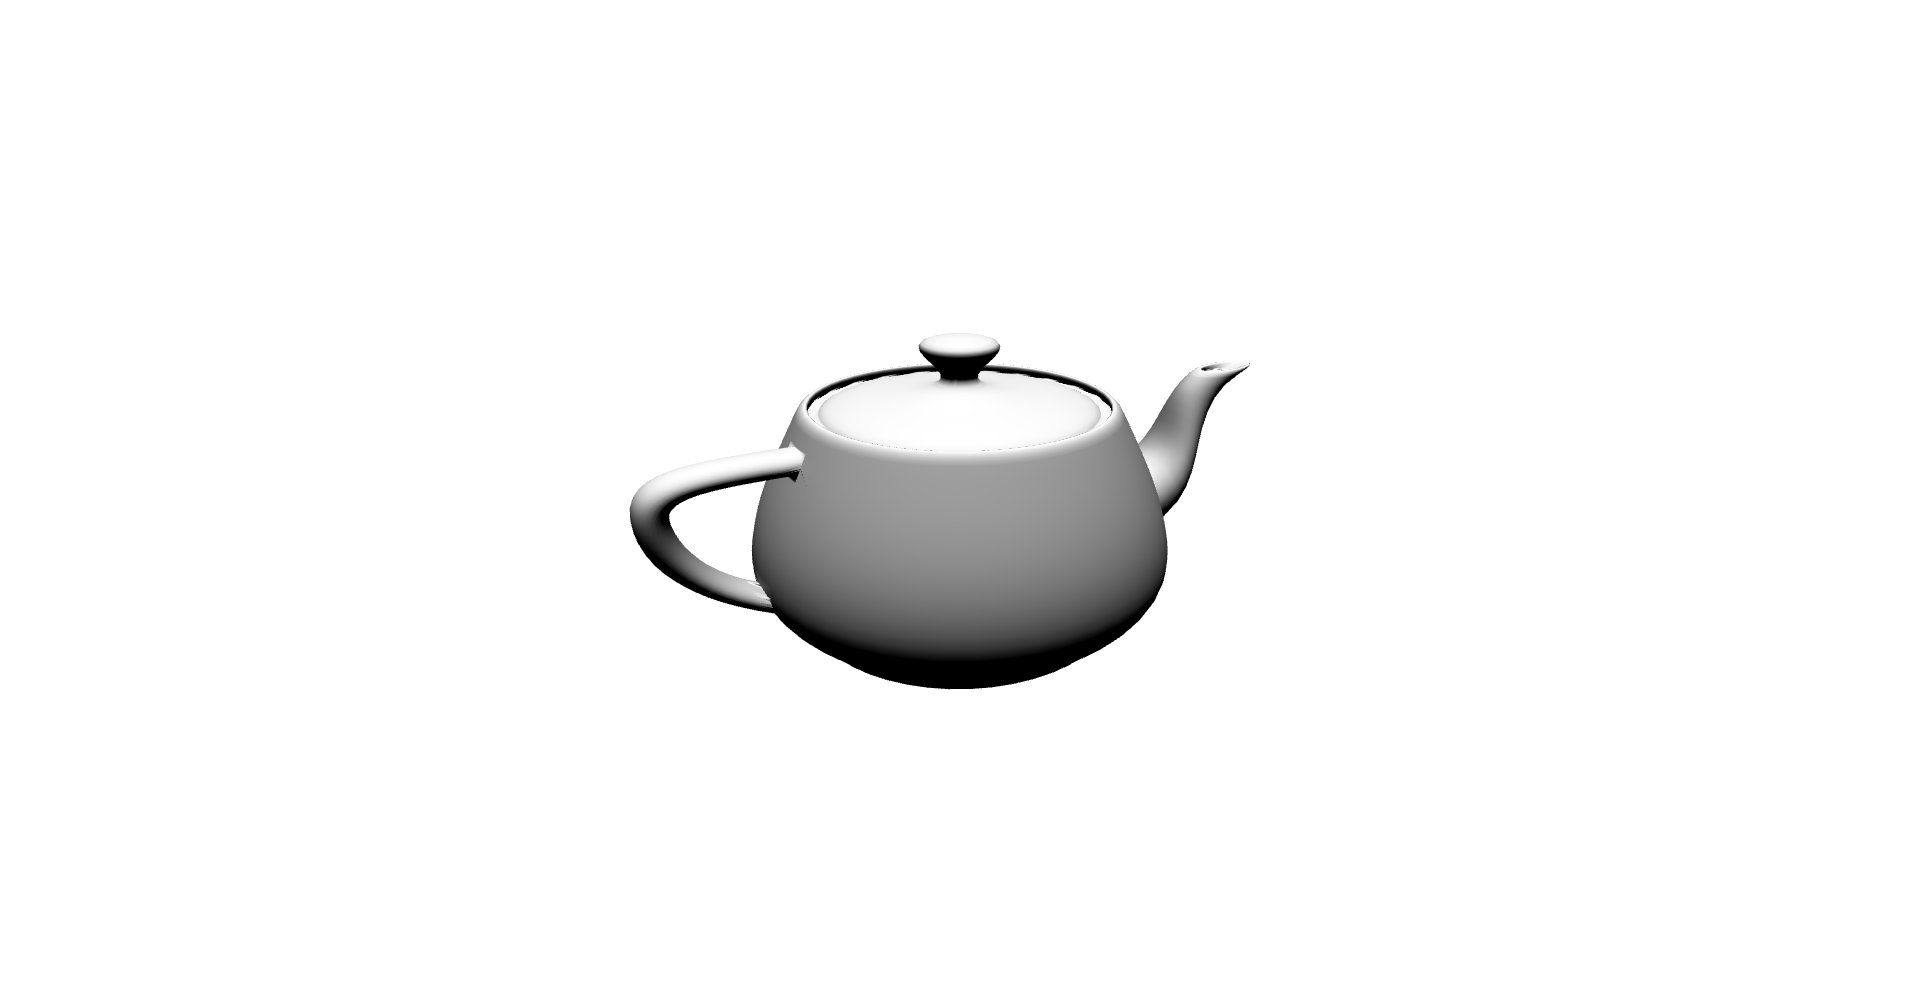
\includegraphics[width=1\linewidth]{teapot/ourLambertTea.png}}
        \caption{Lambert shaded teapot using our implementation.}
        \label{fig:our-lambert-tea}
    \end{subfigure}
    \hfill
    \begin{subfigure}{.48\linewidth}
        \frame{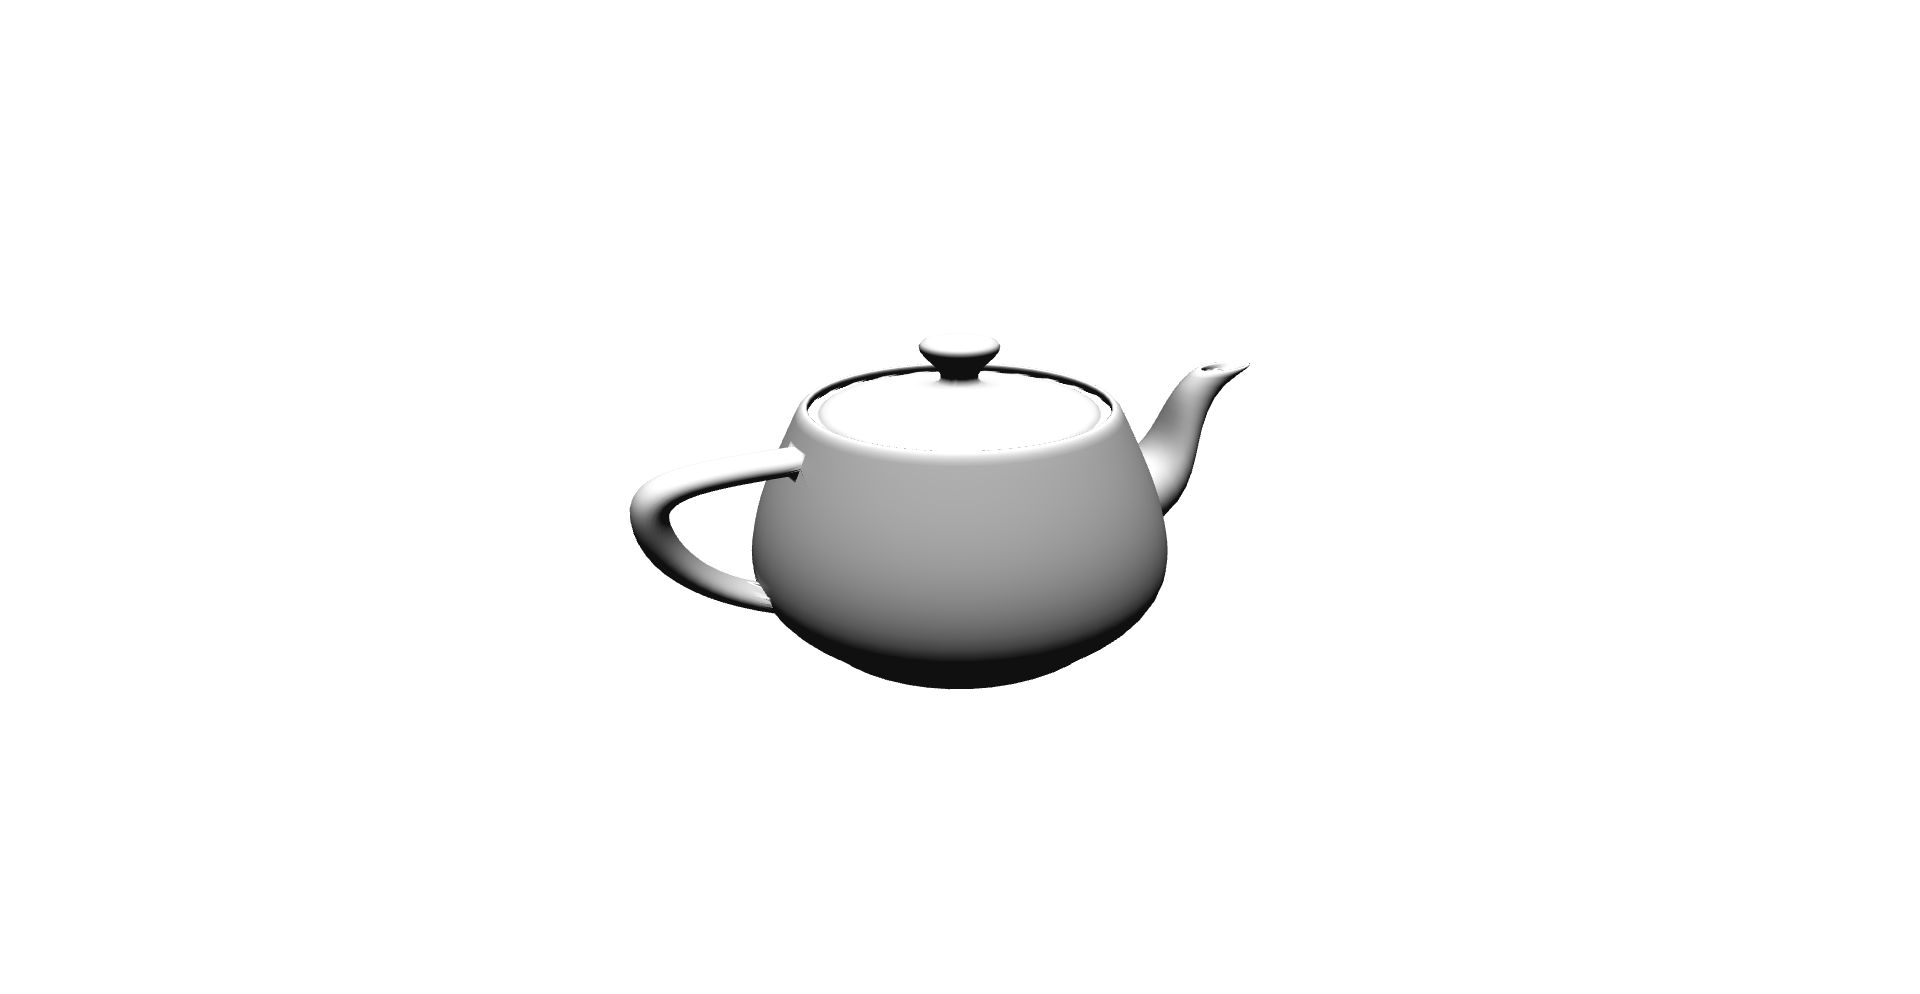
\includegraphics[width=1\linewidth]{teapot/threeLambertTea.png}}
        \caption{Lambert shaded teapot using ThreeJS implementation.}
        \label{fig:three-lambert-tea}
    \end{subfigure}
    \caption{Example of Lambert shading on the Utah Teapot with Phong normals.}
    \label{fig:lambert-tea}
\end{figure*}

\begin{figure*}
    \centering
    \begin{subfigure}{.48\linewidth}
        \frame{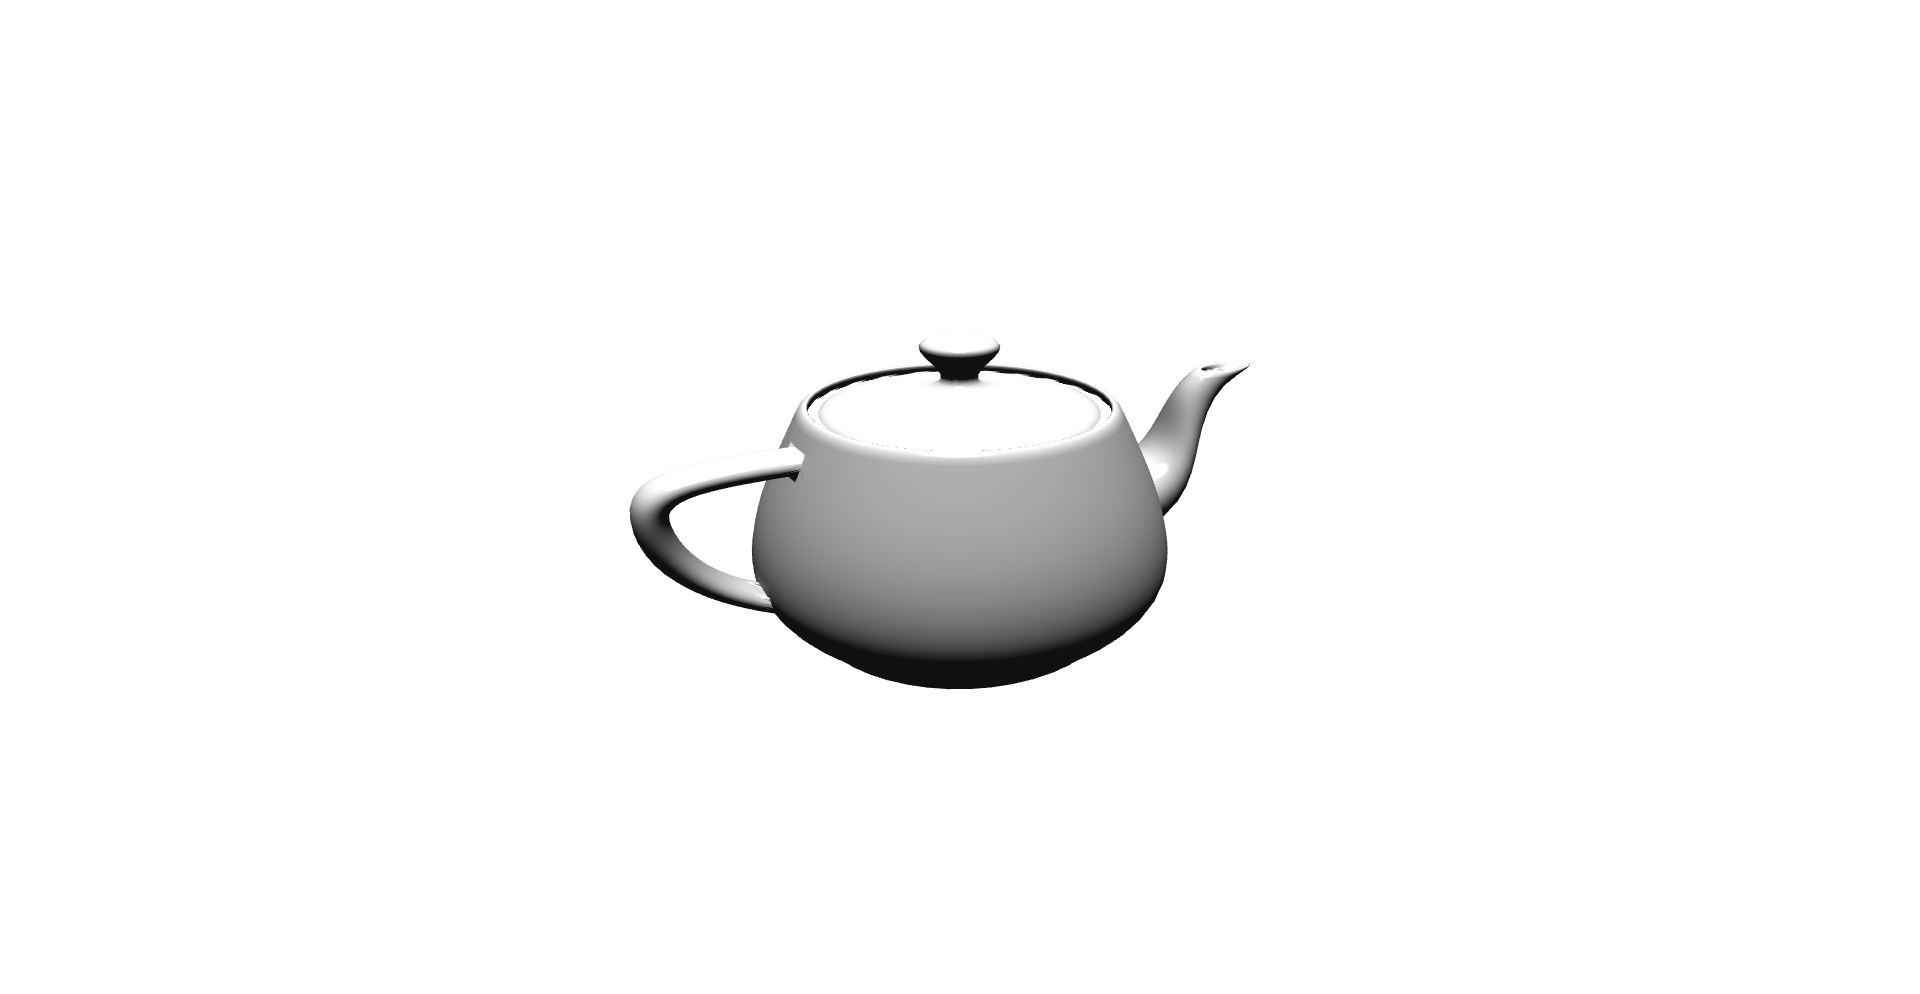
\includegraphics[width=1\linewidth]{teapot/ourPhongTea.png}}
        \caption{Phong shaded teapot using our implementation.}
        \label{fig:our-phong-tea}
    \end{subfigure}
    \hfill
    \begin{subfigure}{.48\linewidth}
        \frame{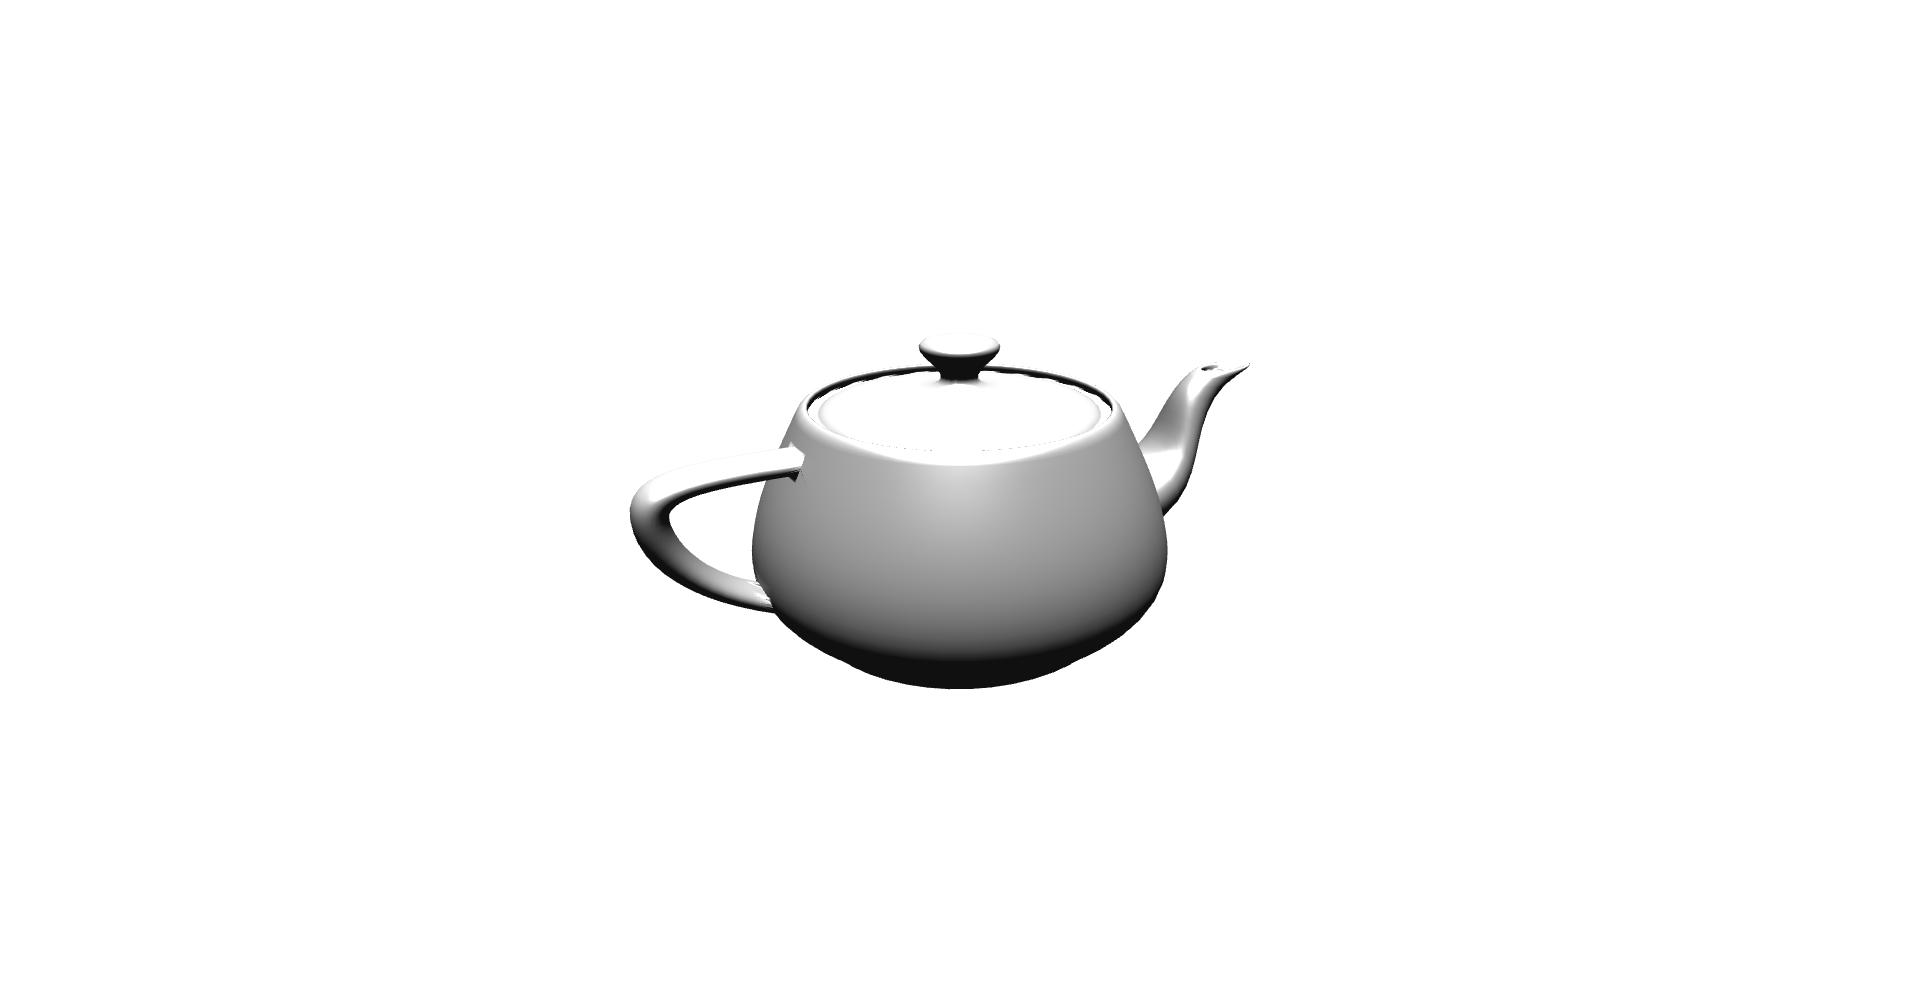
\includegraphics[width=1\linewidth]{teapot/threePhongTea.png}}
        \caption{Phong shaded teapot using ThreeJS implementation.}
        \label{fig:three-phong-tea}
    \end{subfigure}
    \caption{Example of Phong shading on the Utah Teapot, using both Phong normals and Phong lighting. The difference in the amount of shine between implementations becomes more important here. With more complex meshes, different degrees of shine start to dictate which parts of the mesh will shine from certain angles.}
    \label{fig:phong-tea}
\end{figure*}

%--Stanford Lucy--
\begin{figure*}
    \centering
    \begin{subfigure}{.48\linewidth}
        \frame{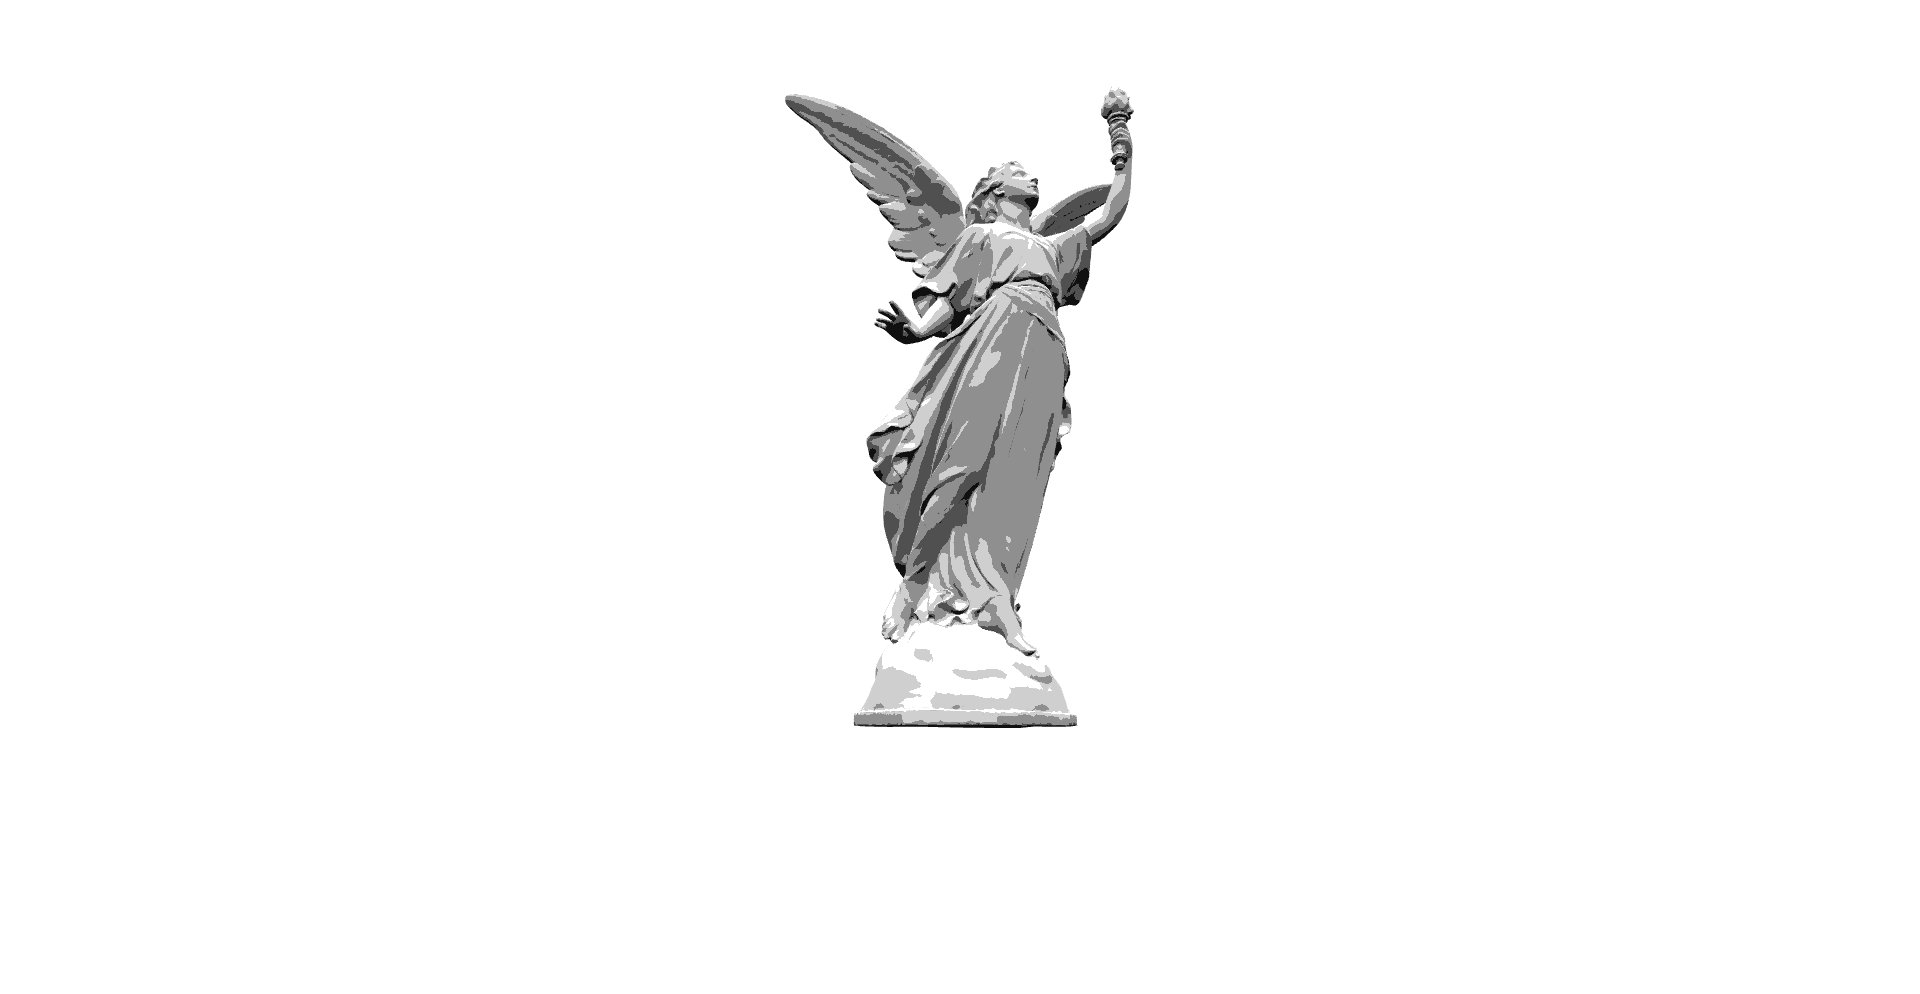
\includegraphics[width=1\linewidth]{lucy/cel.png}}
        \caption{Cel shading on Lucy.}
        \label{fig:lucy-cel}
    \end{subfigure}
    \hfill
    \begin{subfigure}{.48\linewidth}
        \frame{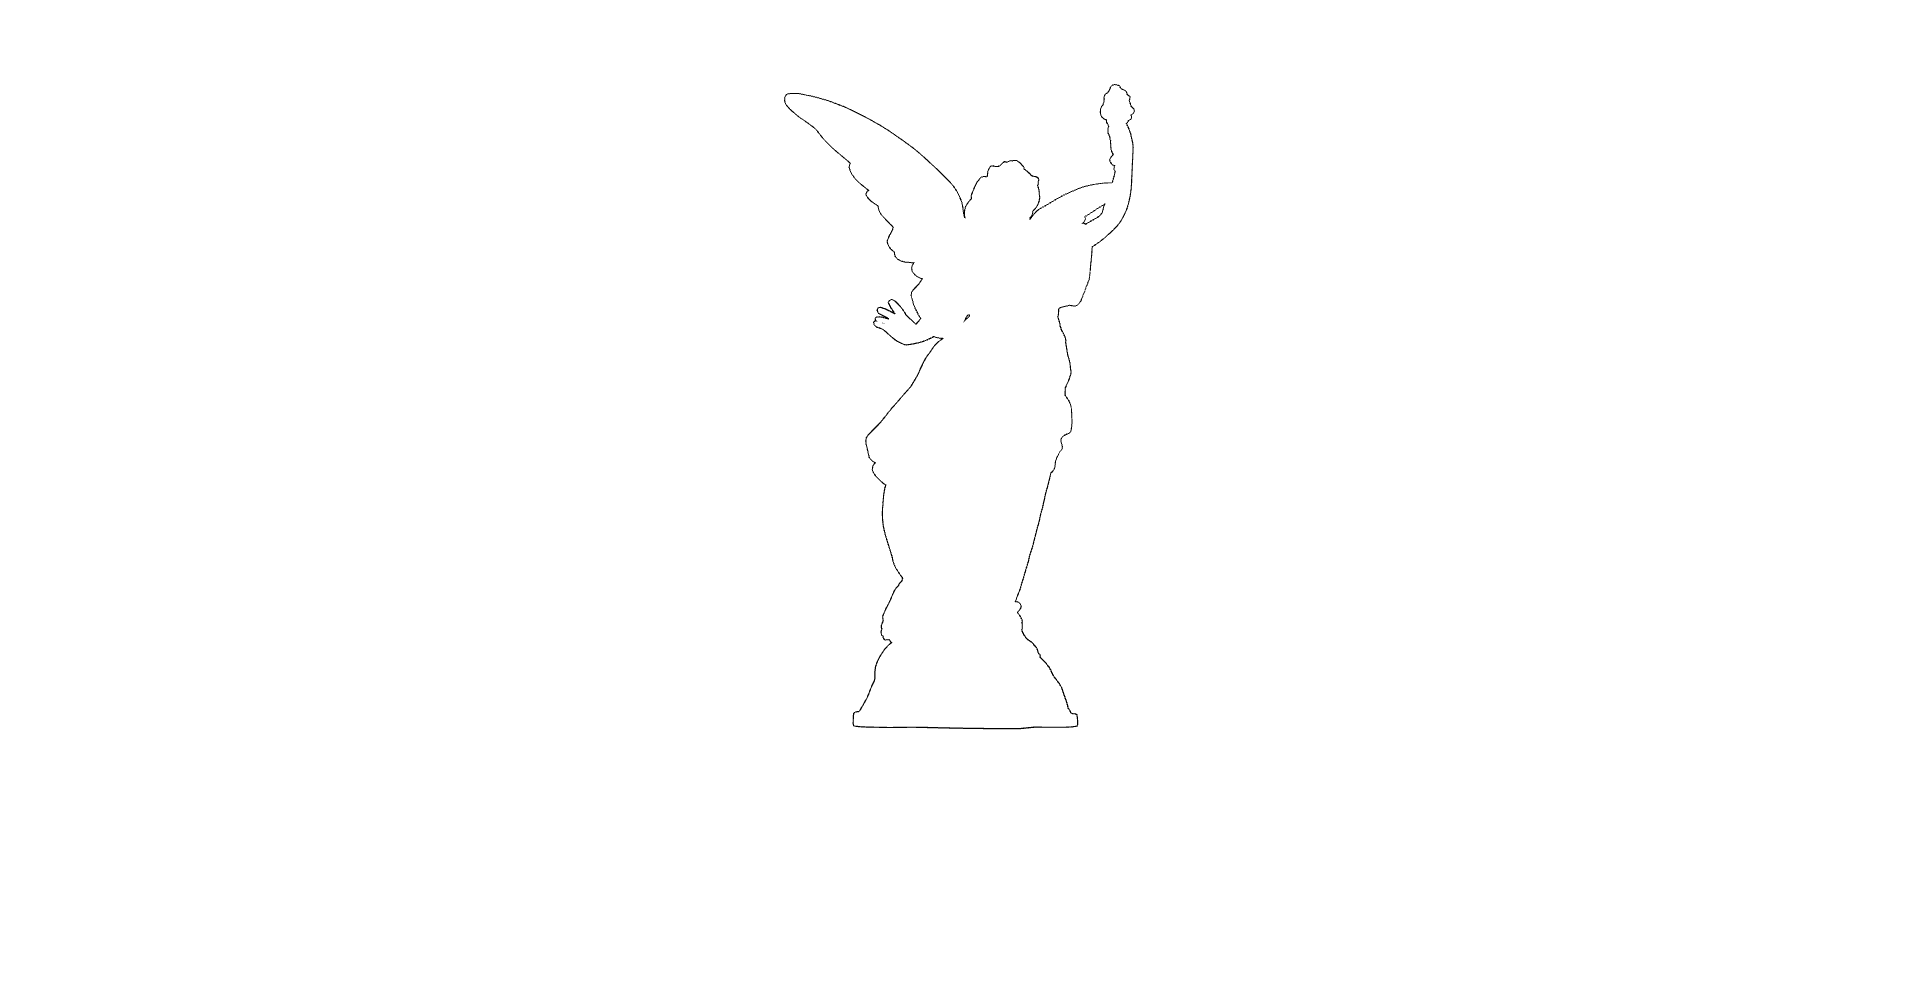
\includegraphics[width=1\linewidth]{lucy/silhouette.png}}
        \caption{Silhouette shading on Lucy.}
        \label{fig:lucy-silhouette}
    \end{subfigure}
    \hfill
    \begin{subfigure}{.48\linewidth}
        \frame{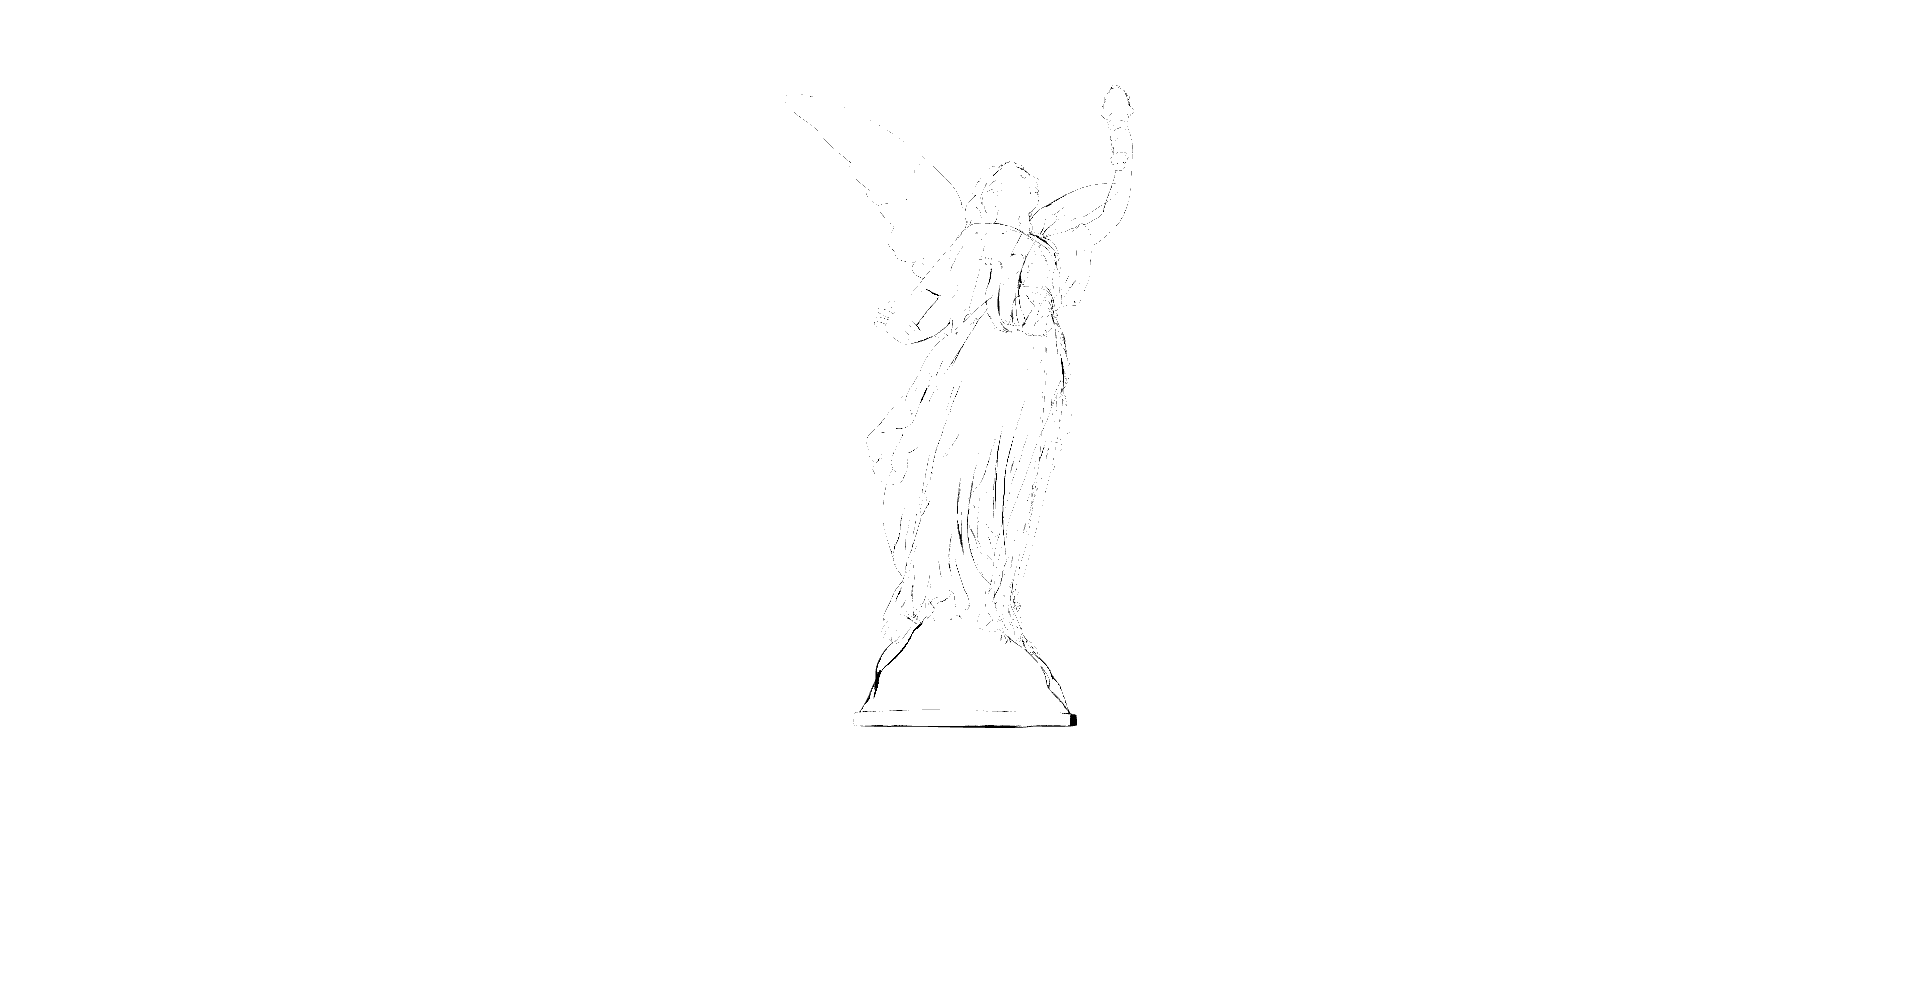
\includegraphics[width=1\linewidth]{lucy/contours.png}}
        \caption{Contour shading on Lucy.}
        \label{fig:lucy-contours}
    \end{subfigure}
    \hfill
    \begin{subfigure}{.48\linewidth}
        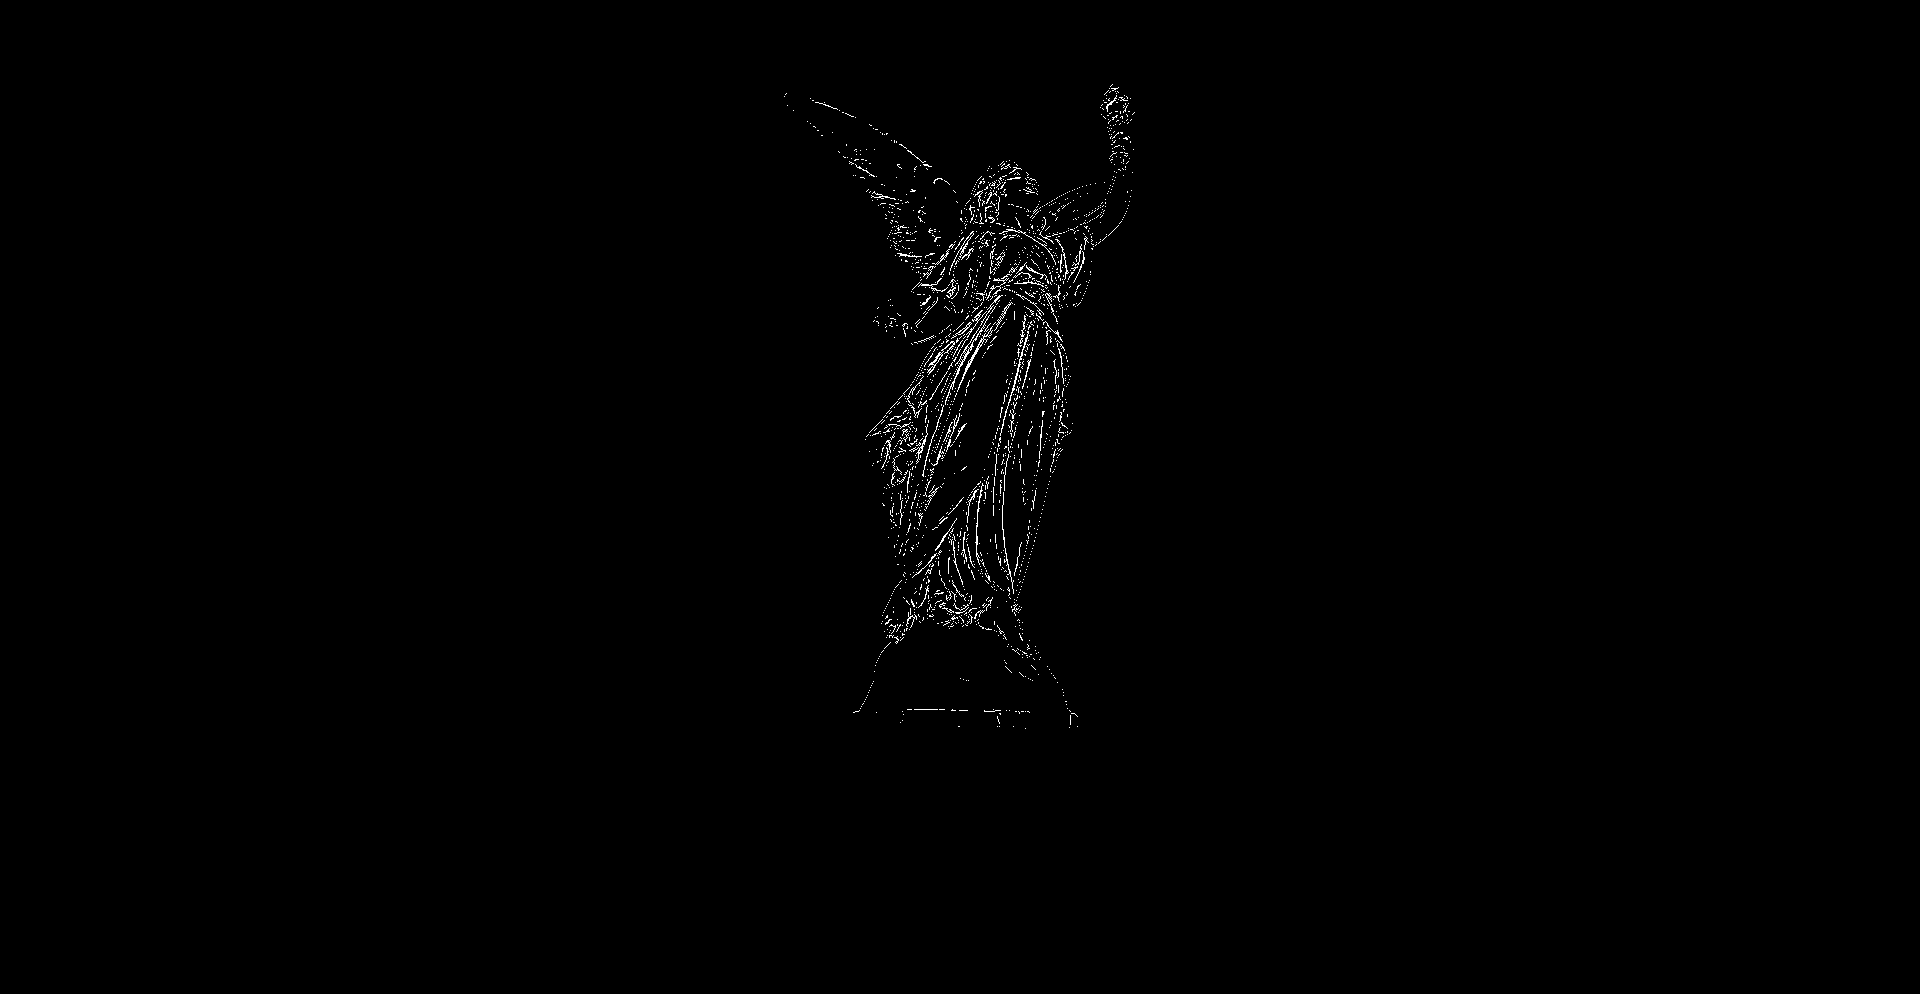
\includegraphics[width=1\linewidth]{lucy/sugg_contours.png}
        \caption{Final pass of the suggestive contour shader applied on Lucy.}
        \label{fig:lucy-suggs}
    \end{subfigure}
    \hfill
    \begin{subfigure}{1\linewidth}
        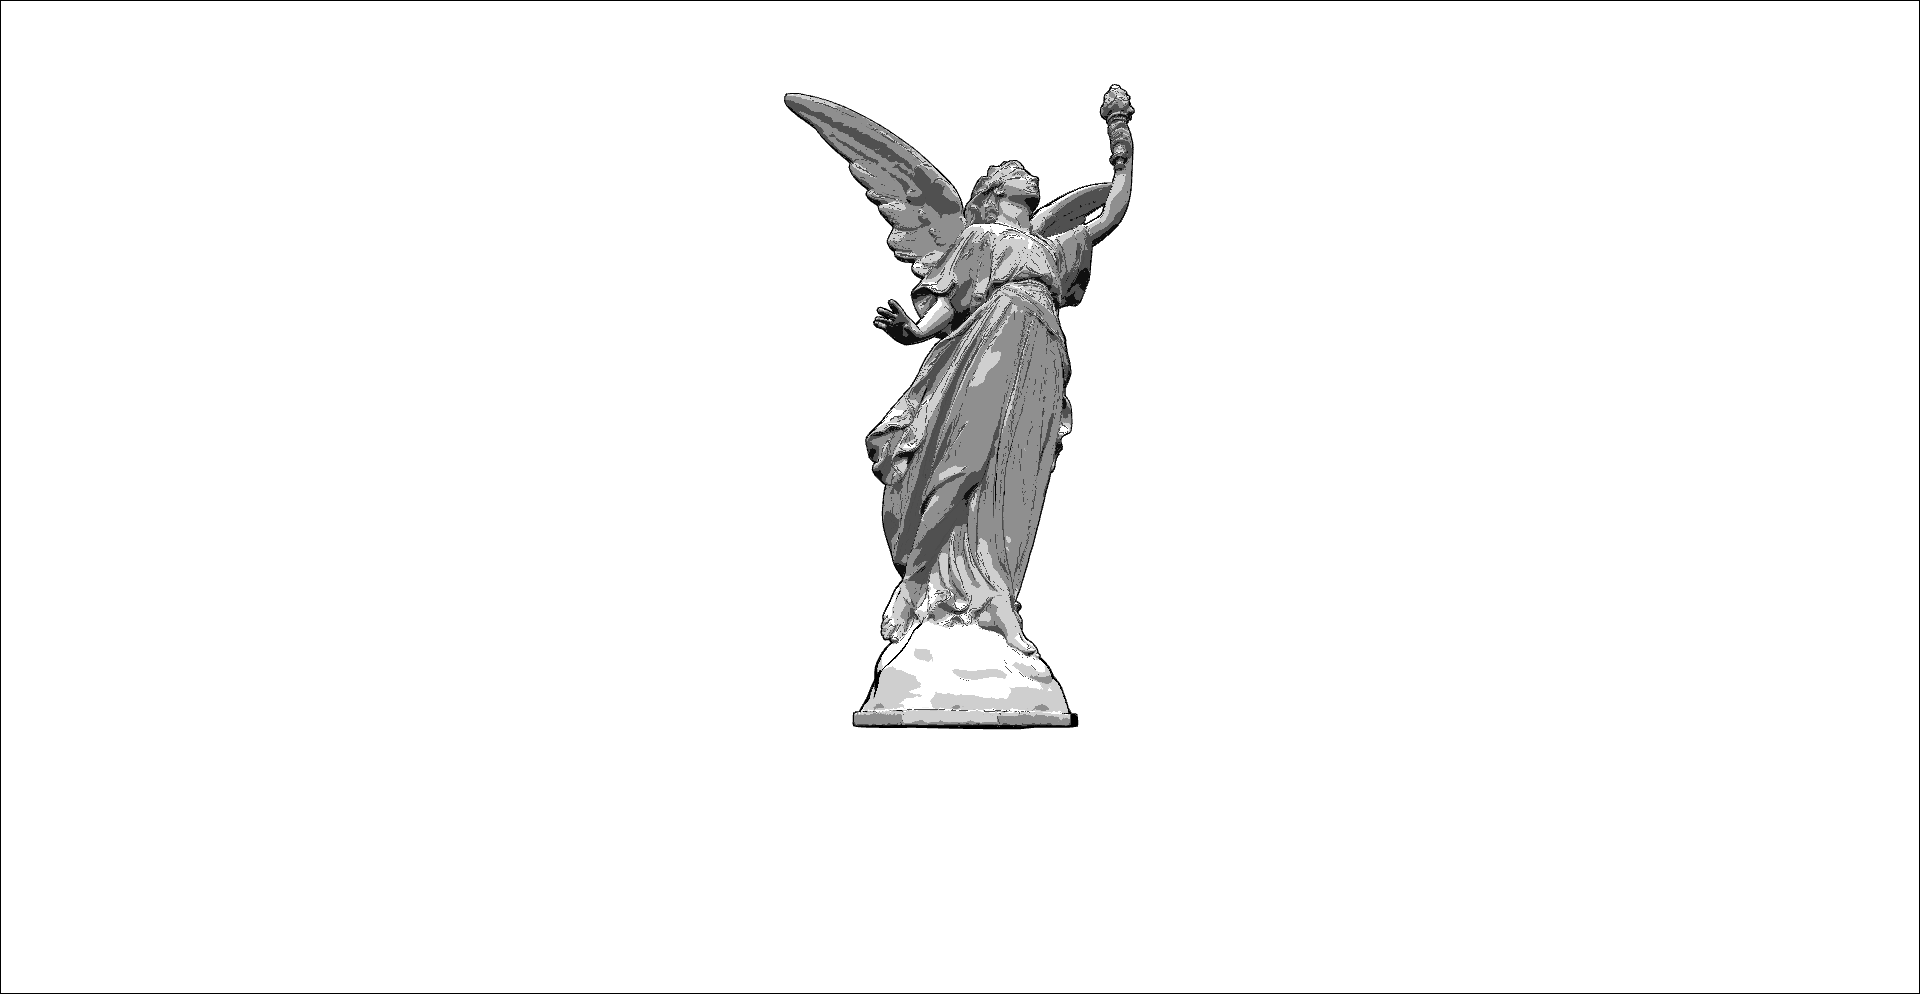
\includegraphics[width=1\linewidth]{lucy/final.png}
        \caption{All four of the nonphotorealistic shading techniques being applied to Lucy simultaneously.}
        \label{fig:lucy-anime}
    \end{subfigure}
    \caption{Example of the nonphotorealistic shaders being applied to the Stanford Lucy model both individually and simultaneously. As you can see, the image seems to have a lot of extra lines drawn especially on the face of the figure}
    \label{fig:lucy}
\end{figure*}

%--Ajax Bust--
\begin{figure*}
    \centering
    \begin{subfigure}{.48\linewidth}
        \frame{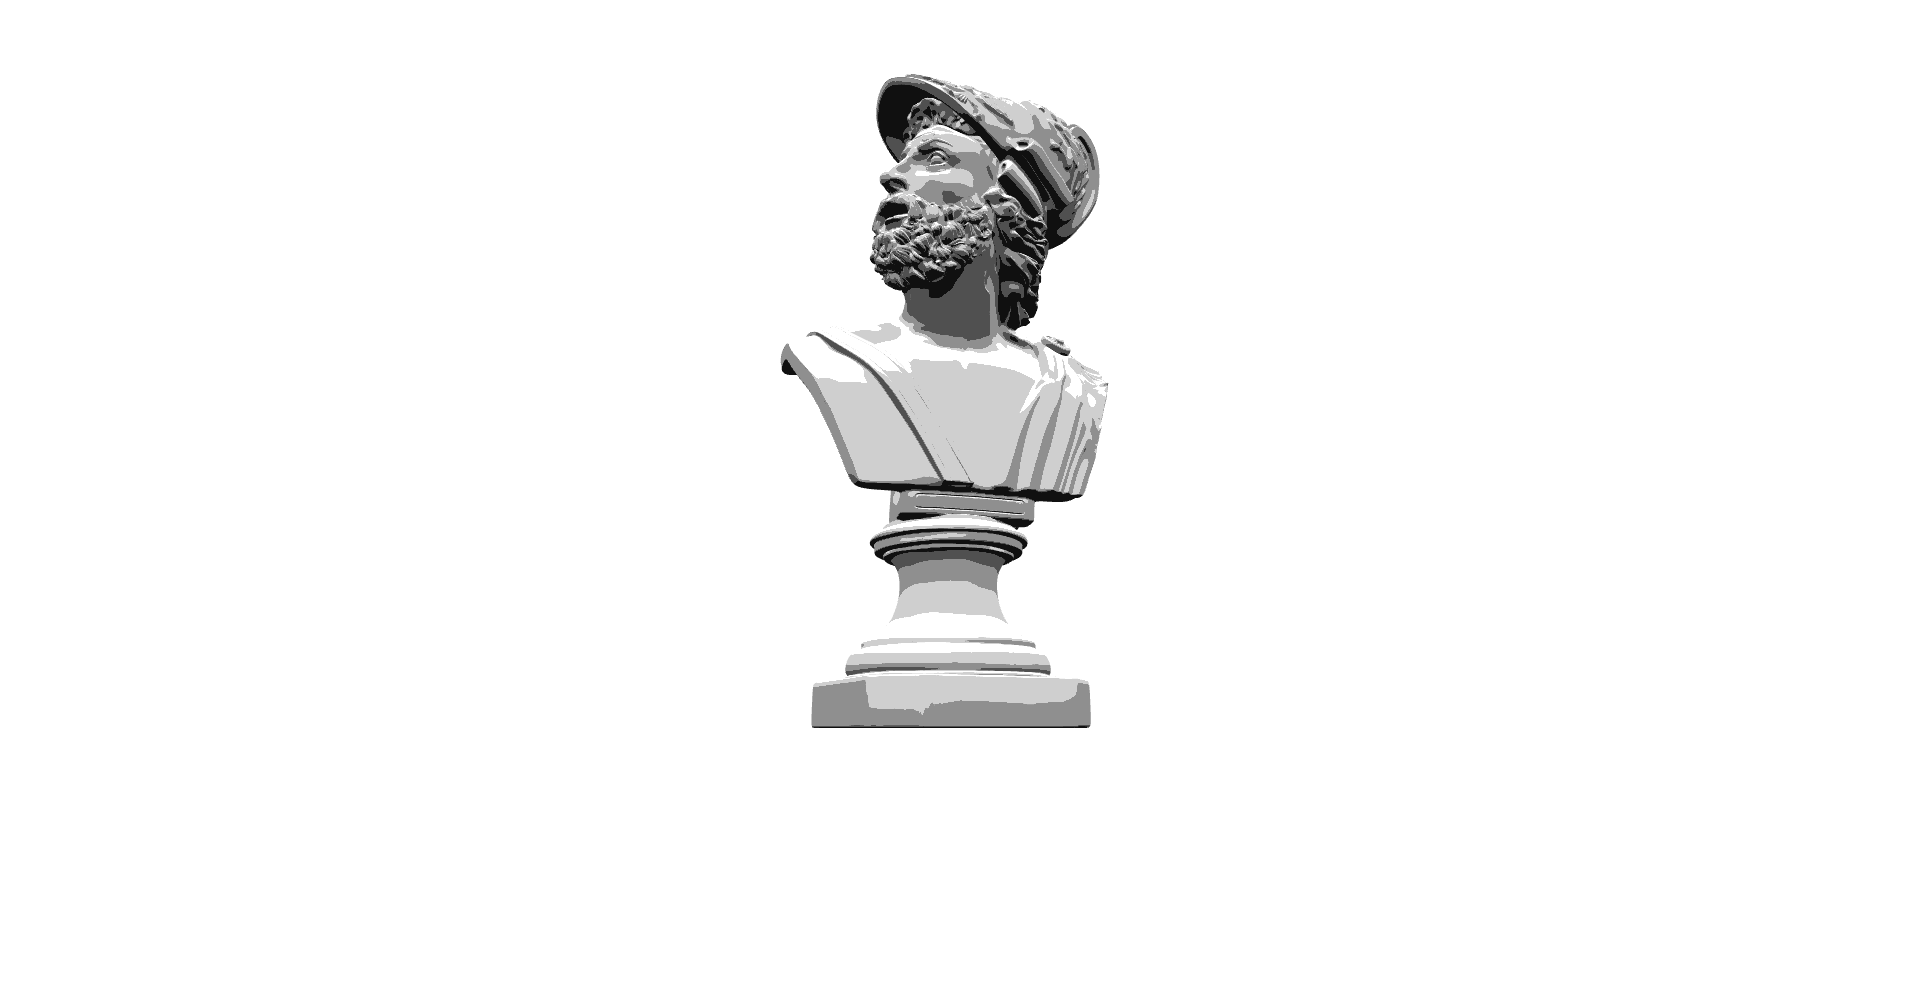
\includegraphics[width=1\linewidth]{ajax/cel.png}}
        \caption{Cel shading on Ajax.}
        \label{fig:ajax-cel}
    \end{subfigure}
    \hfill
    \begin{subfigure}{.48\linewidth}
        \frame{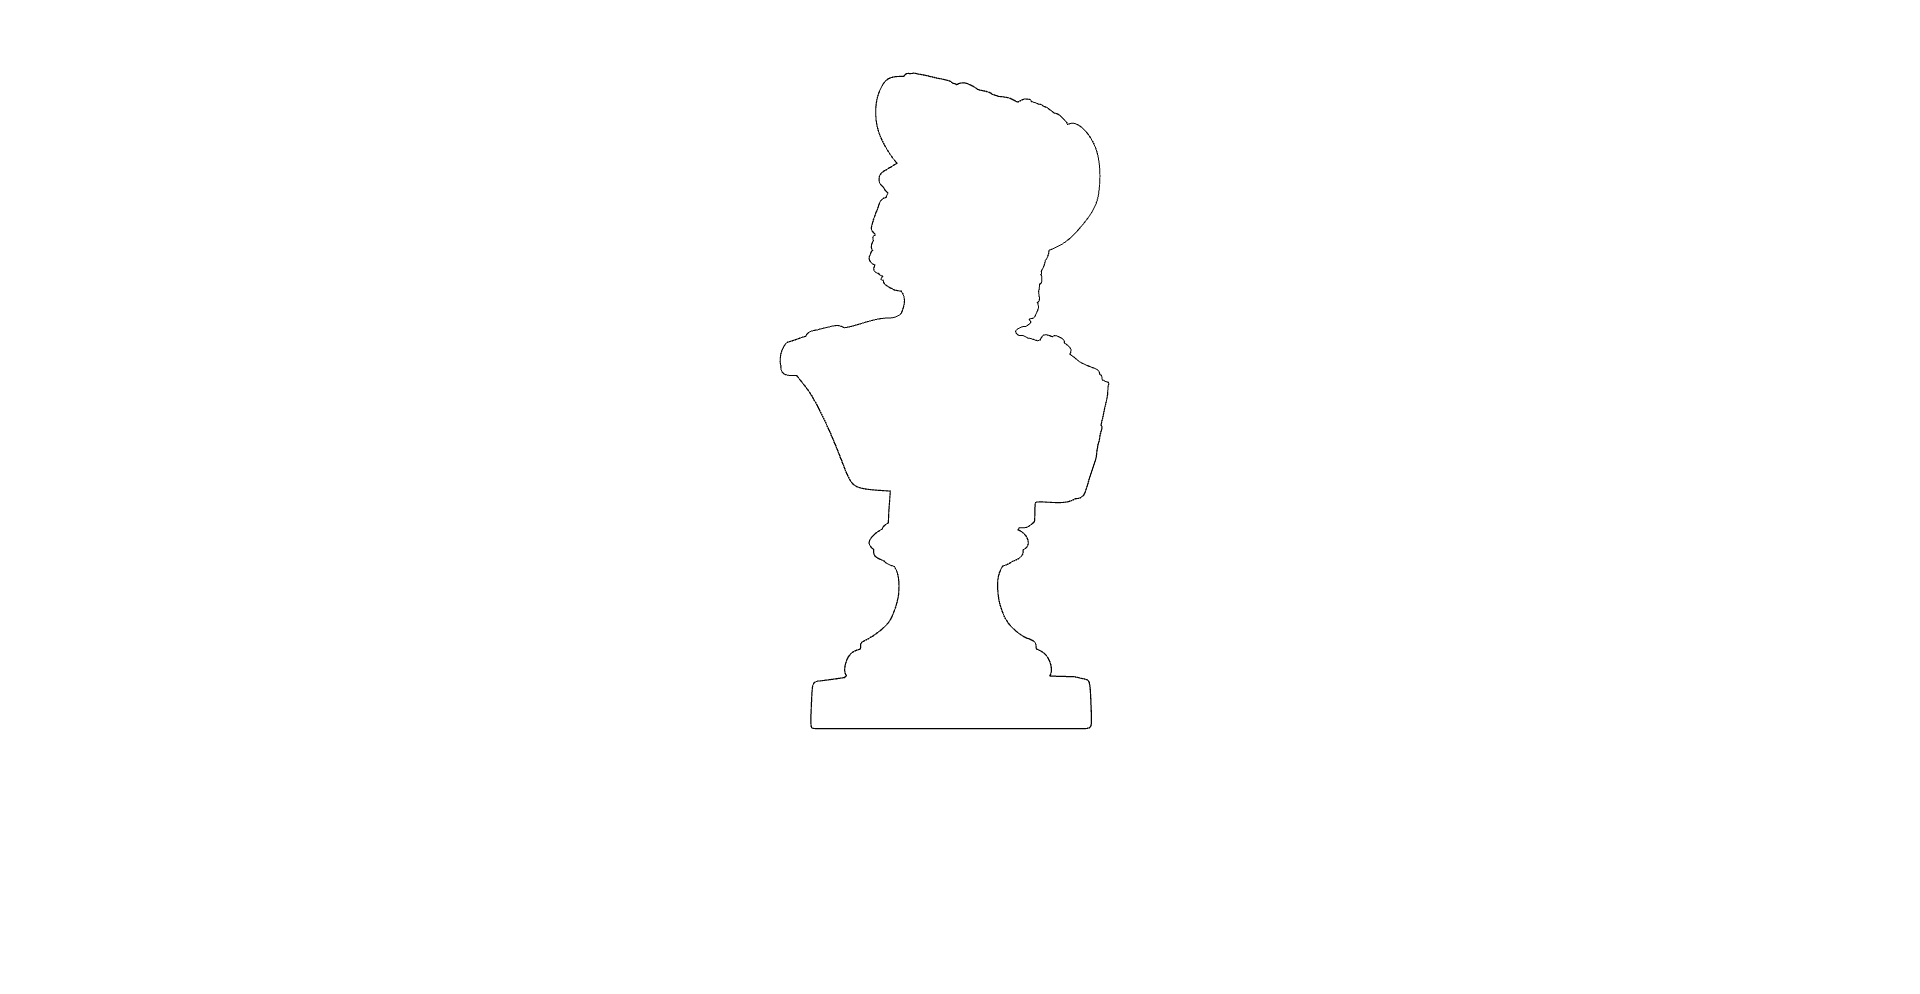
\includegraphics[width=1\linewidth]{ajax/silhouette.png}}
        \caption{Silhouette shading on Ajax.}
        \label{fig:ajax-silhouette}
    \end{subfigure}
    \hfill
    \begin{subfigure}{.48\linewidth}
        \frame{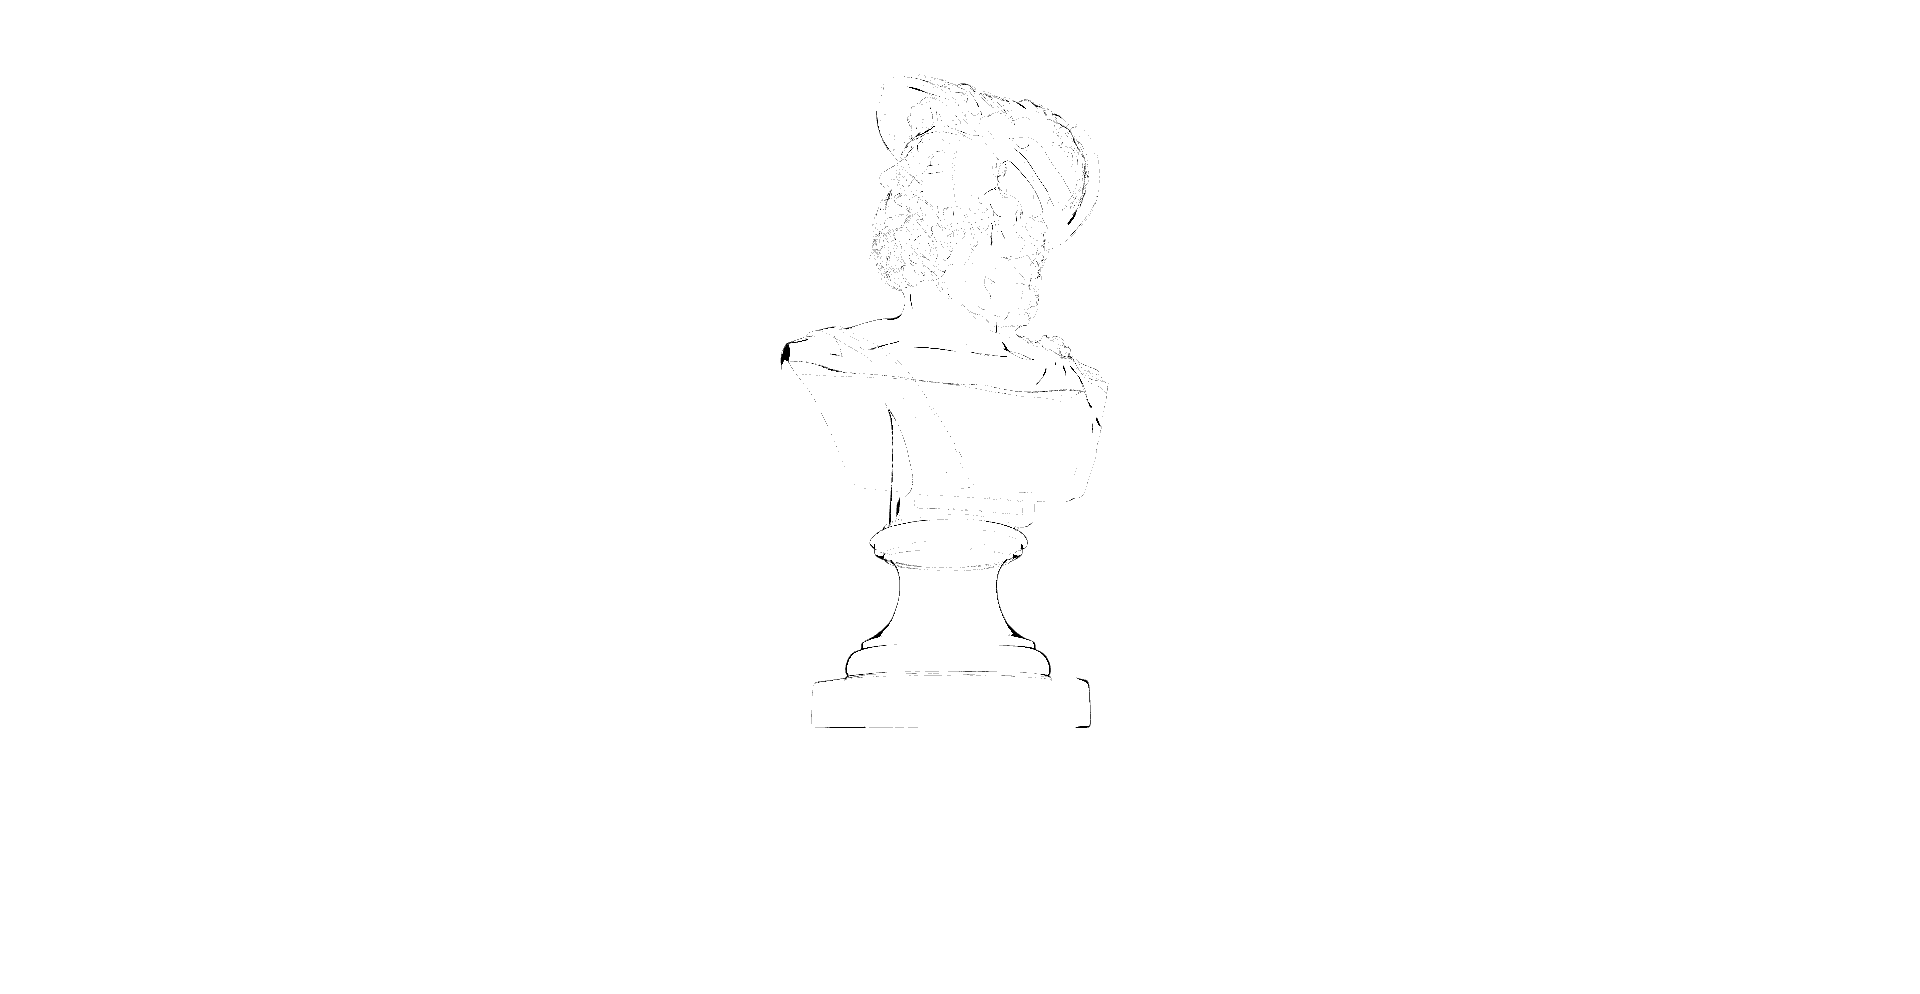
\includegraphics[width=1\linewidth]{ajax/contours.png}}
        \caption{Contour shading on Ajax.}
        \label{fig:ajax-contours}
    \end{subfigure}
    \hfill
    \begin{subfigure}{.48\linewidth}
        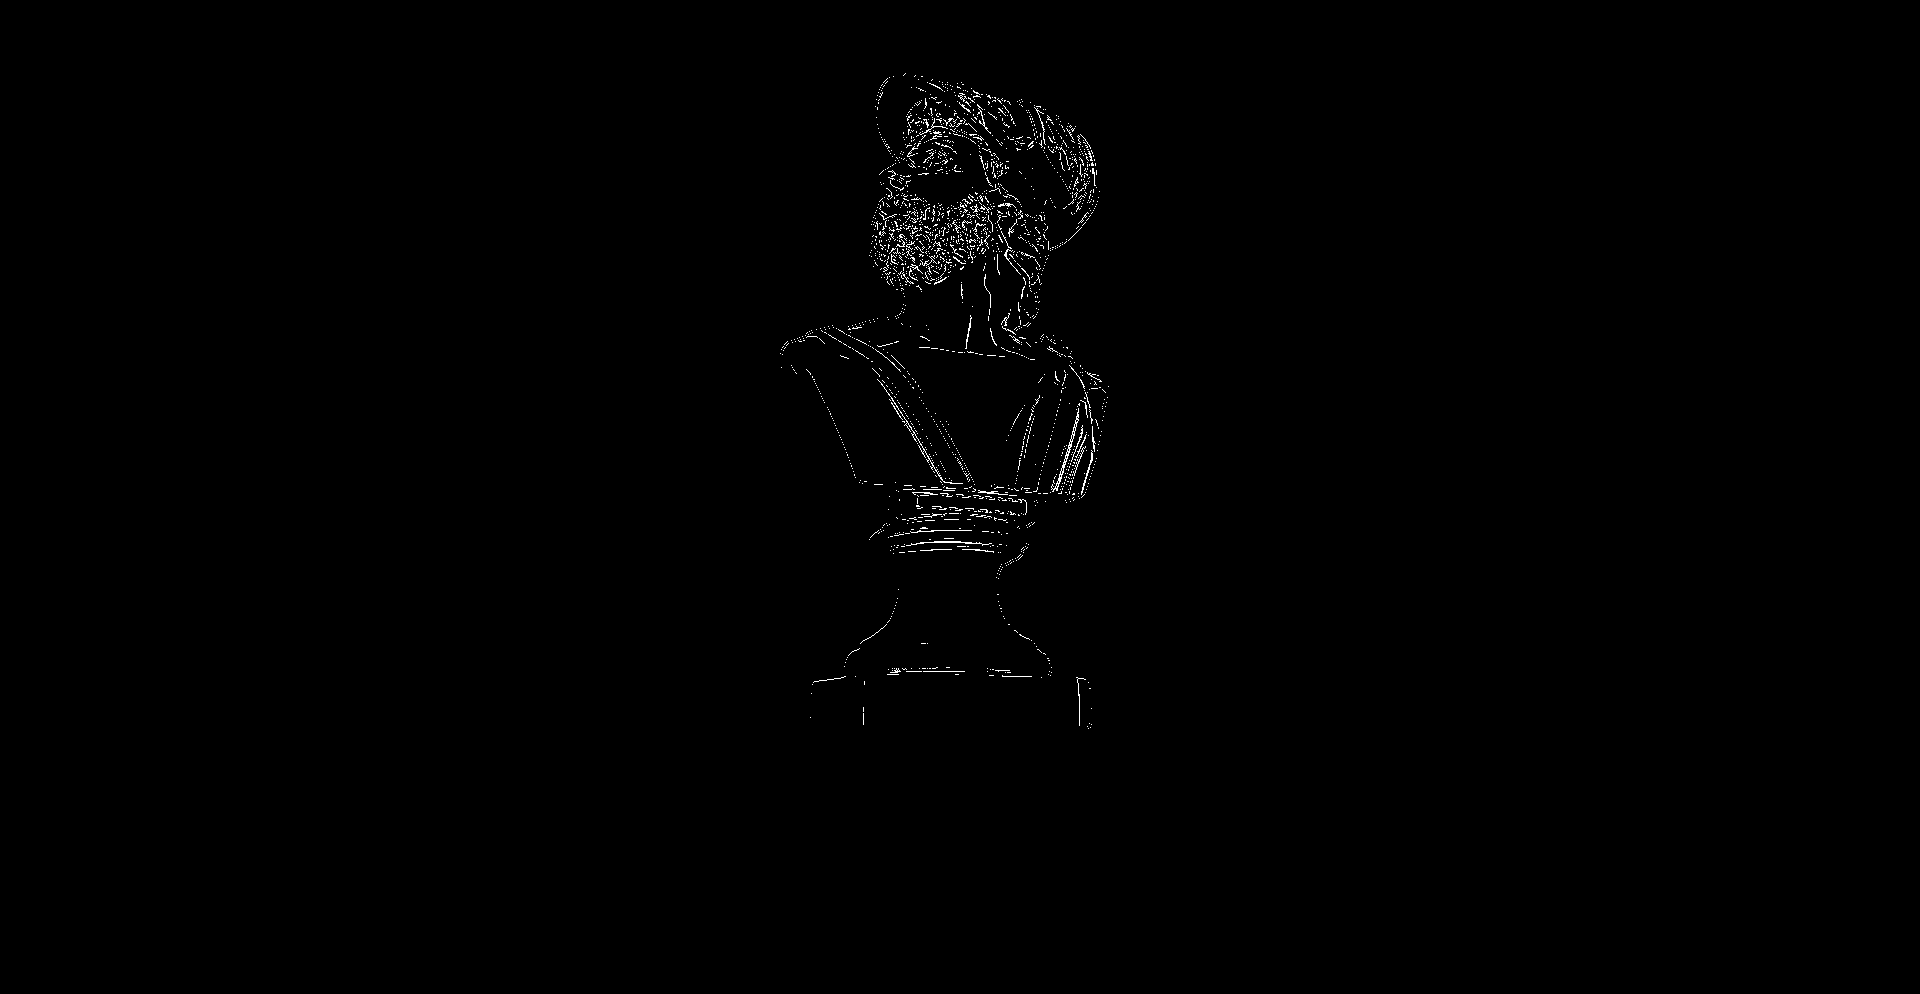
\includegraphics[width=1\linewidth]{ajax/sugg_contours.png}
        \caption{Final pass of the suggestive contour shader applied on Ajax.}
        \label{fig:ajax-suggs}
    \end{subfigure}
    \hfill
    \begin{subfigure}{1\linewidth}
        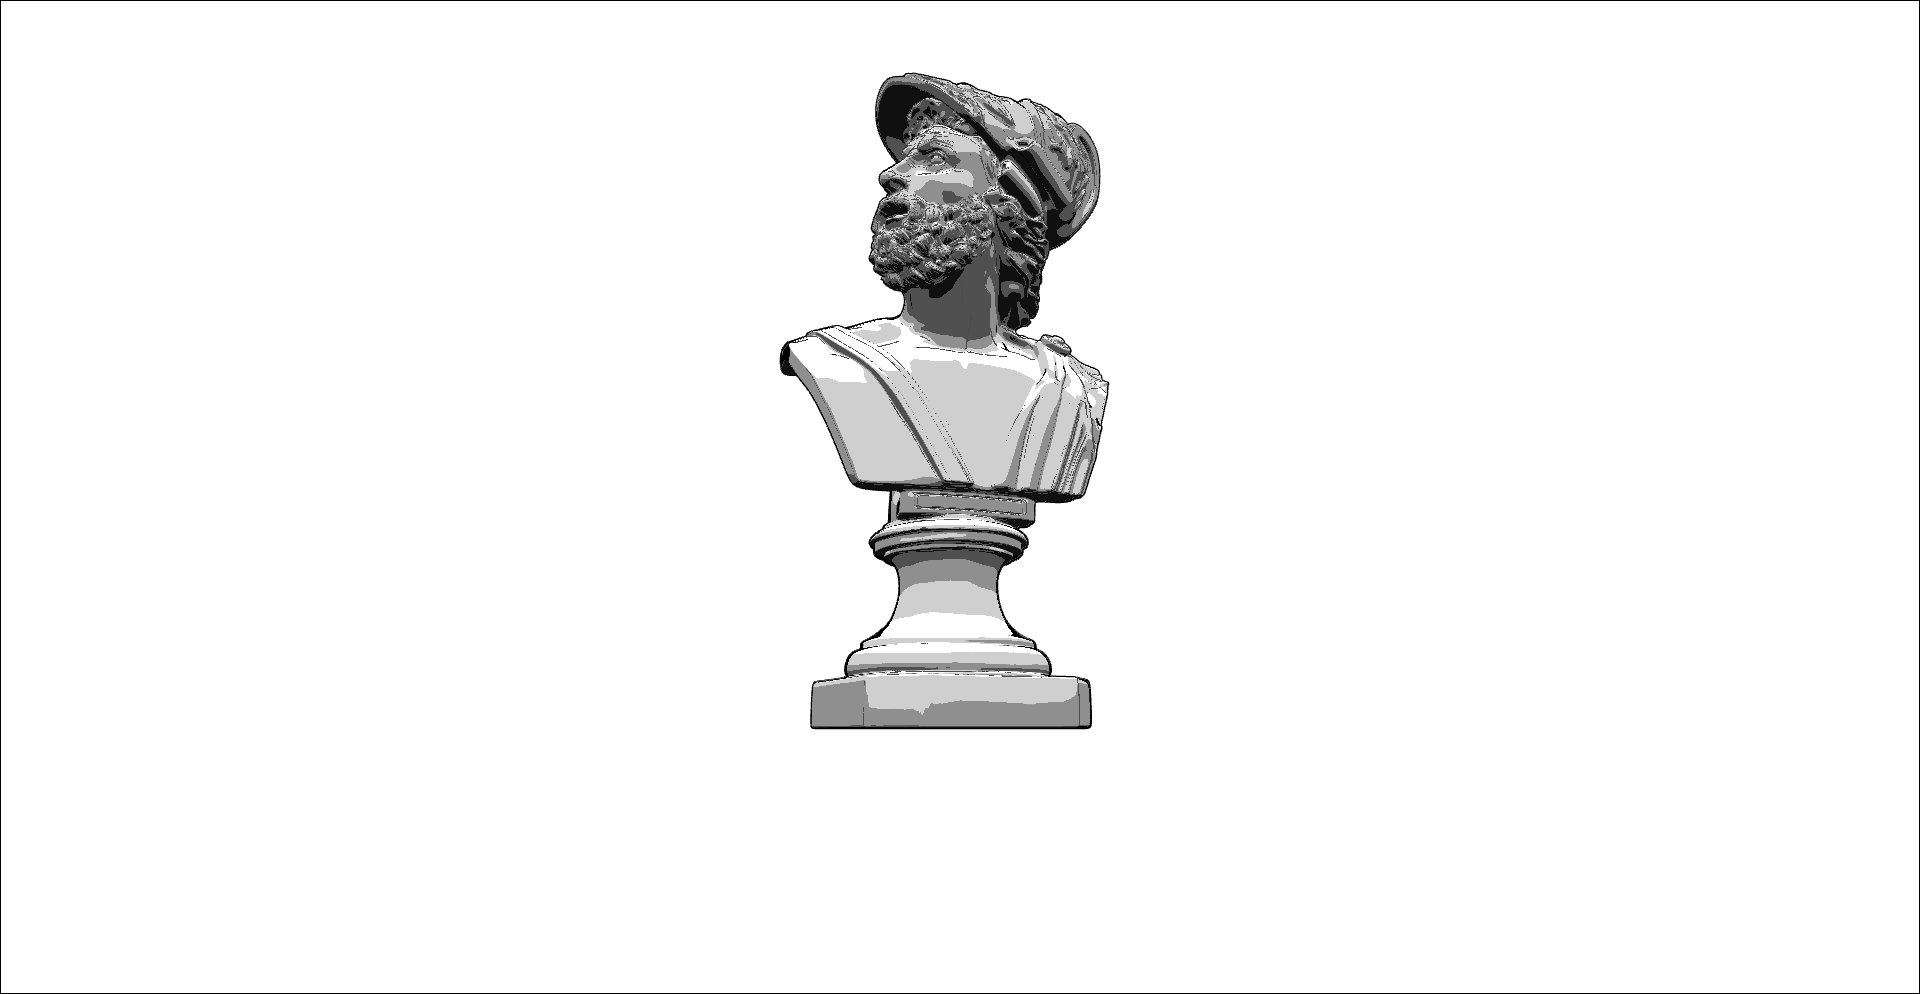
\includegraphics[width=1\linewidth]{ajax/final.png}
        \caption{All four of the nonphotorealistic shading techniques being applied to Ajax simultaneously.}
        \label{fig:ajax-anime}
    \end{subfigure}
    \caption{Example of the nonphotorealistic shaders being applied to the Ajax bust model both individually and simultaneously. As you can see, the image seems to have a lot of extra lines drawn especially on the face of the figure.}
    \label{fig:ajax}
\end{figure*}



% \setlength{\belowcaptionskip}{0pt}
% \setlength{\abovecaptionskip}{-10pt}


%--Lucy Comparison--
\begin{figure*}
    \centering
    \begin{subfigure}{.48\linewidth}
        \frame{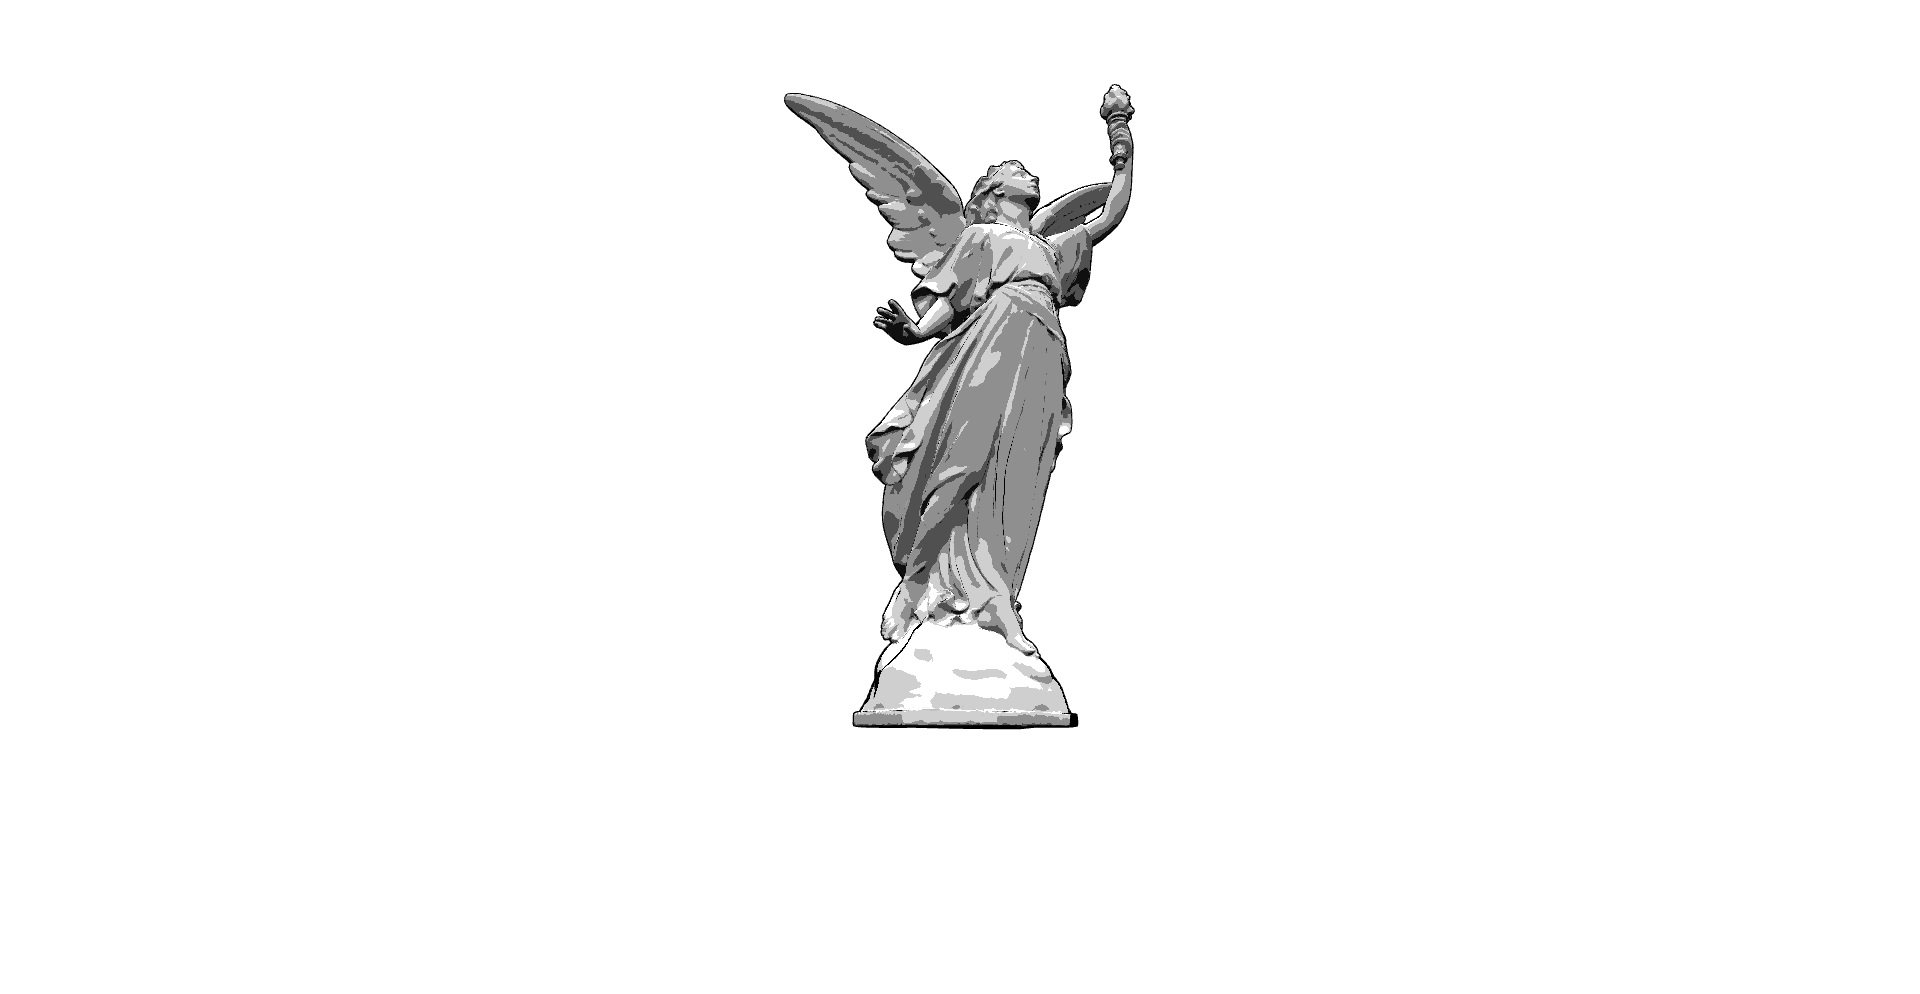
\includegraphics[width=1\linewidth]{lucy/base.png}}
        \caption{Lucy drawn without suggestive contours.}
        \label{fig:lucy-base}
    \end{subfigure}
    \hfill
    \begin{subfigure}{.48\linewidth}
        \frame{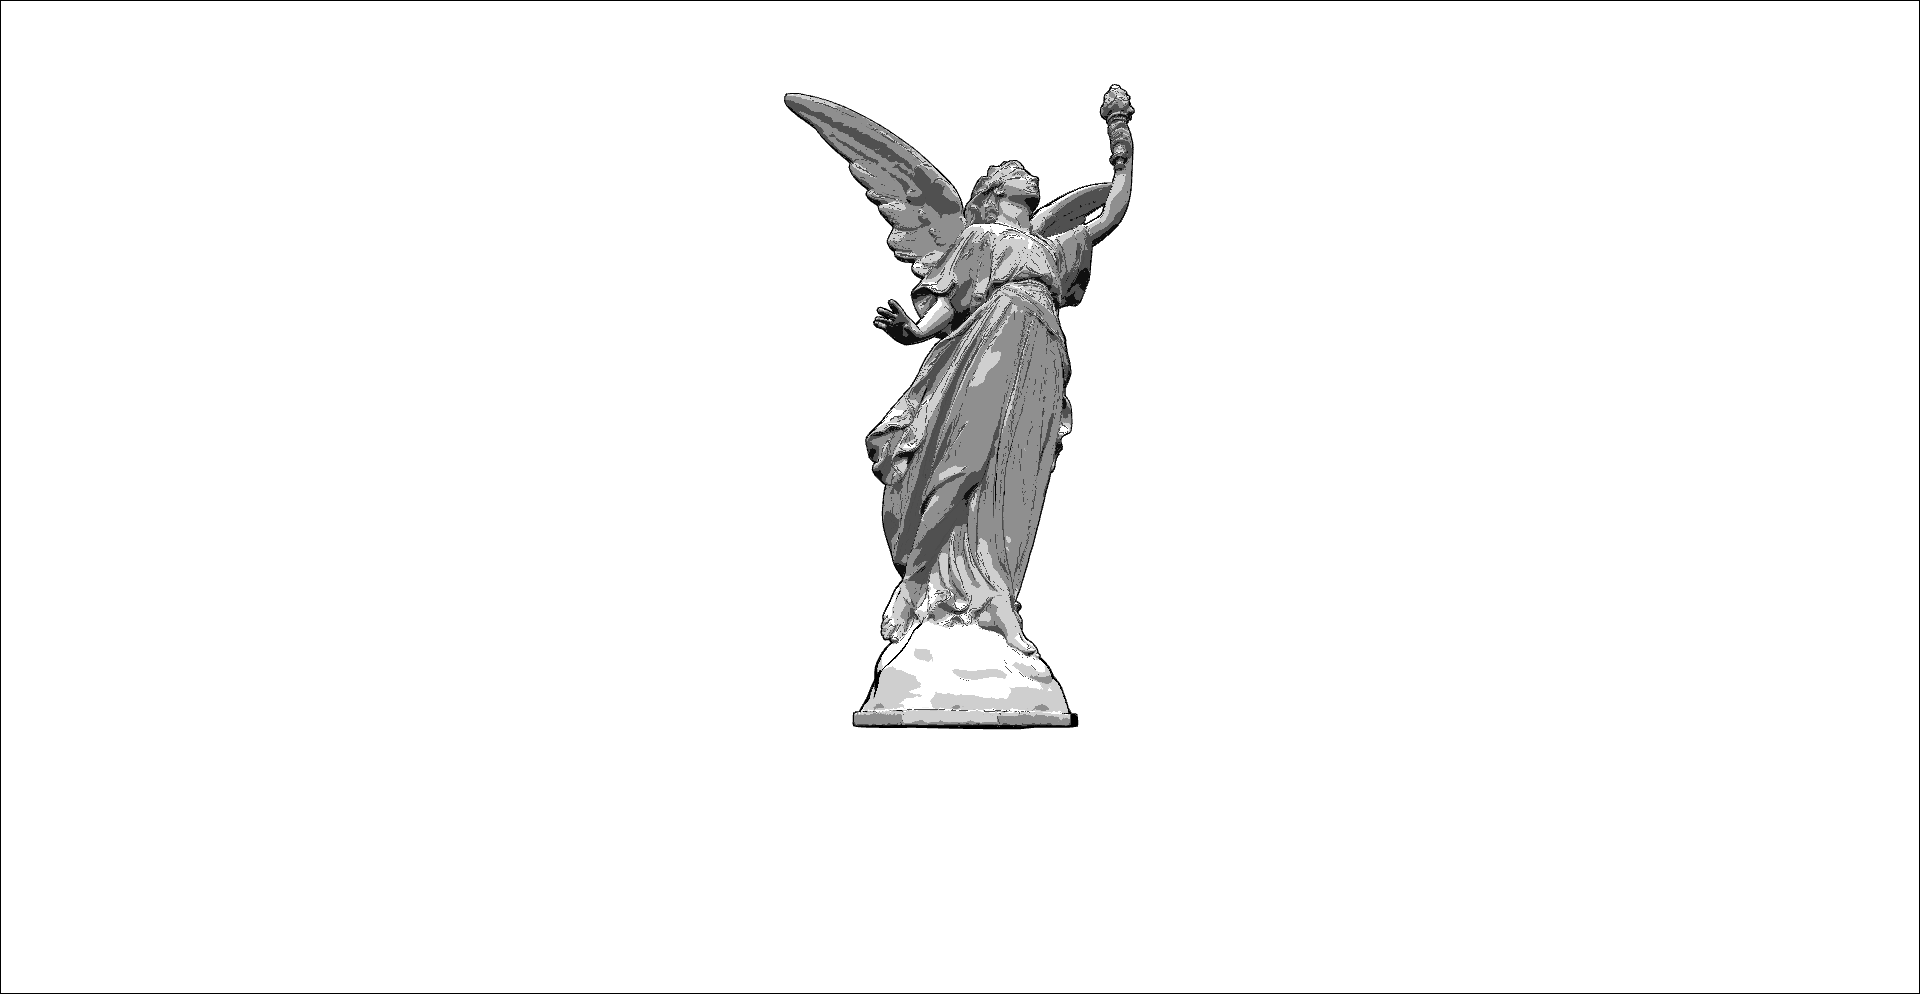
\includegraphics[width=1\linewidth]{lucy/final.png}}
        \caption{Lucy drawn with suggestive contours.}
        \label{fig:lucy-final}
    \end{subfigure}
    \caption{Comparing Lucy drawn with all nonphotorealistic shading techniques with and without suggestive contours to see which result creates a more cortoon-ish image.}
    \label{fig:lucy-compare}
\end{figure*}

%--Ajax Comparison--
\begin{figure*}
    \centering
    \begin{subfigure}{.48\linewidth}
        \frame{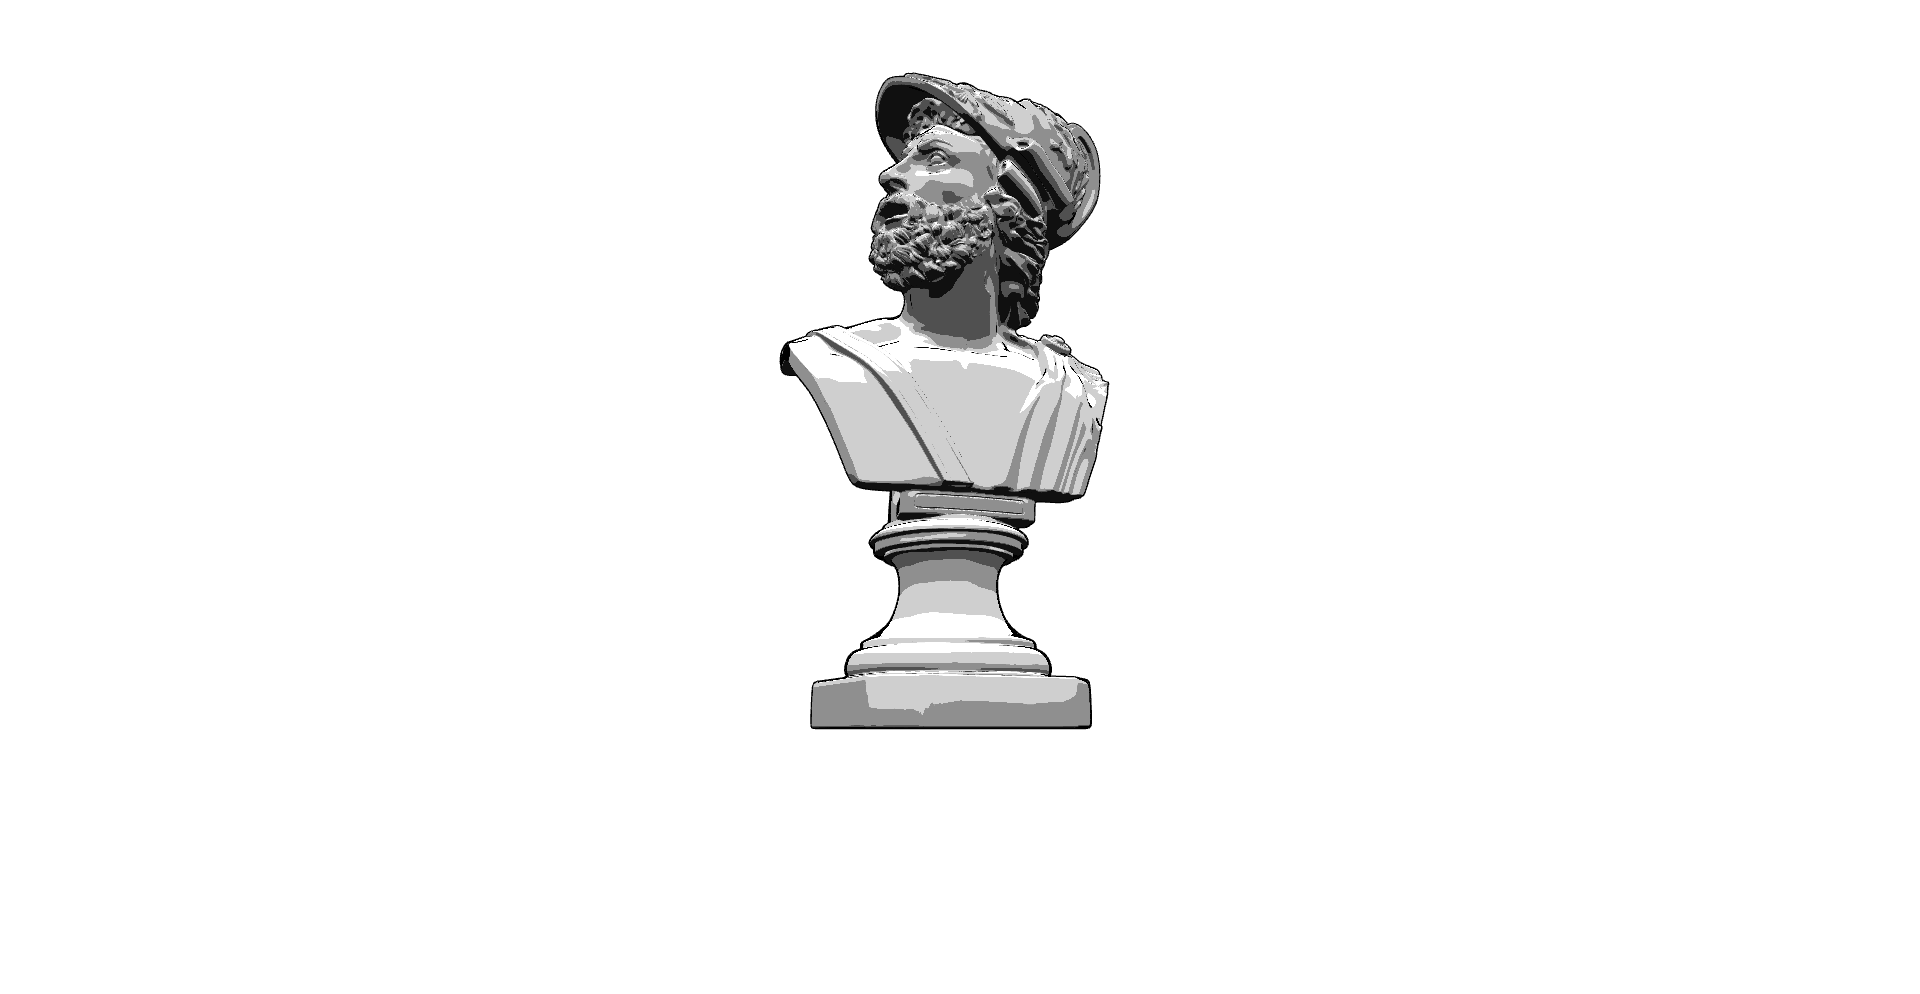
\includegraphics[width=1\linewidth]{ajax/base.png}}
        \caption{Ajax drawn without suggestive contours.}
        \label{fig:ajax-base}
    \end{subfigure}
    \hfill
    \begin{subfigure}{.48\linewidth}
        \frame{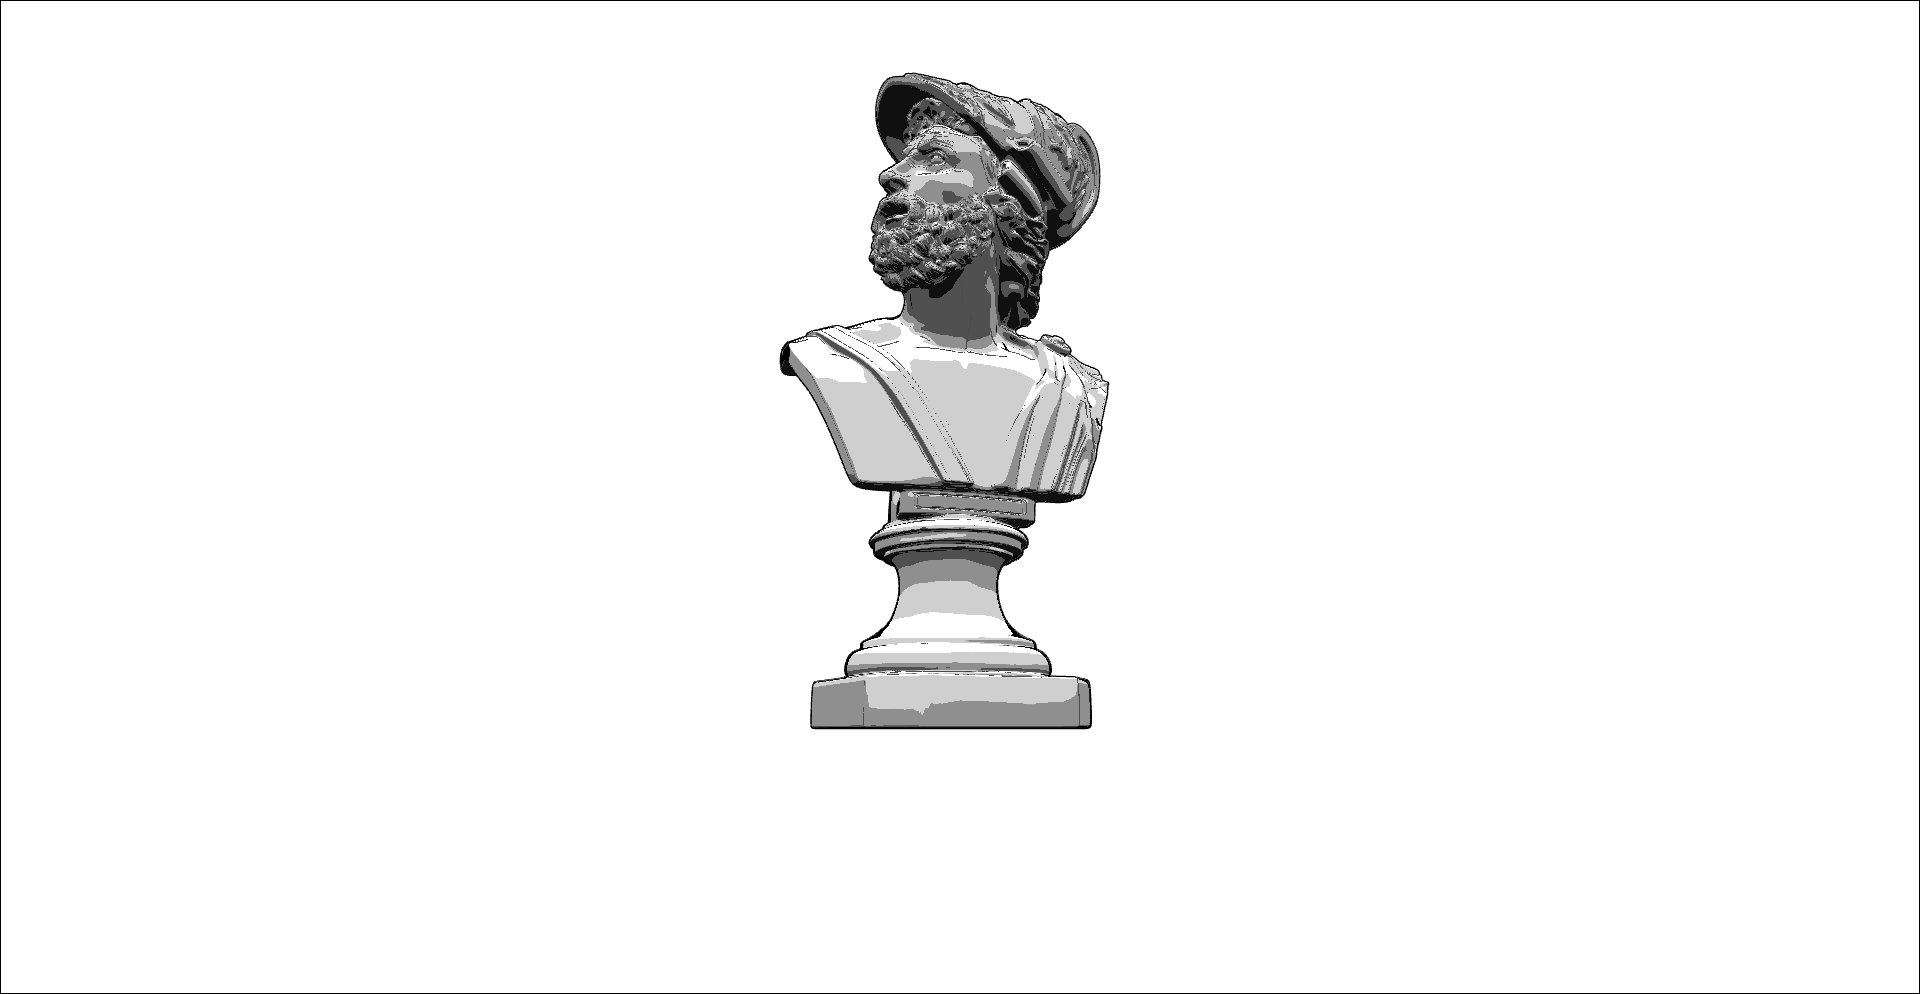
\includegraphics[width=1\linewidth]{ajax/final.png}}
        \caption{Ajax drawn with suggestive contours.}
        \label{fig:ajax-final}
    \end{subfigure}
    \caption{Comparing Ajax drawn with all nonphotorealistic shading techniques with and without suggestive contours to see which result creates a more cortoon-ish image.}
    \label{fig:ajax-compare}
\end{figure*}

%--Amber Comparison--
\begin{figure*}
    \centering
    \begin{subfigure}{.48\linewidth}
        \frame{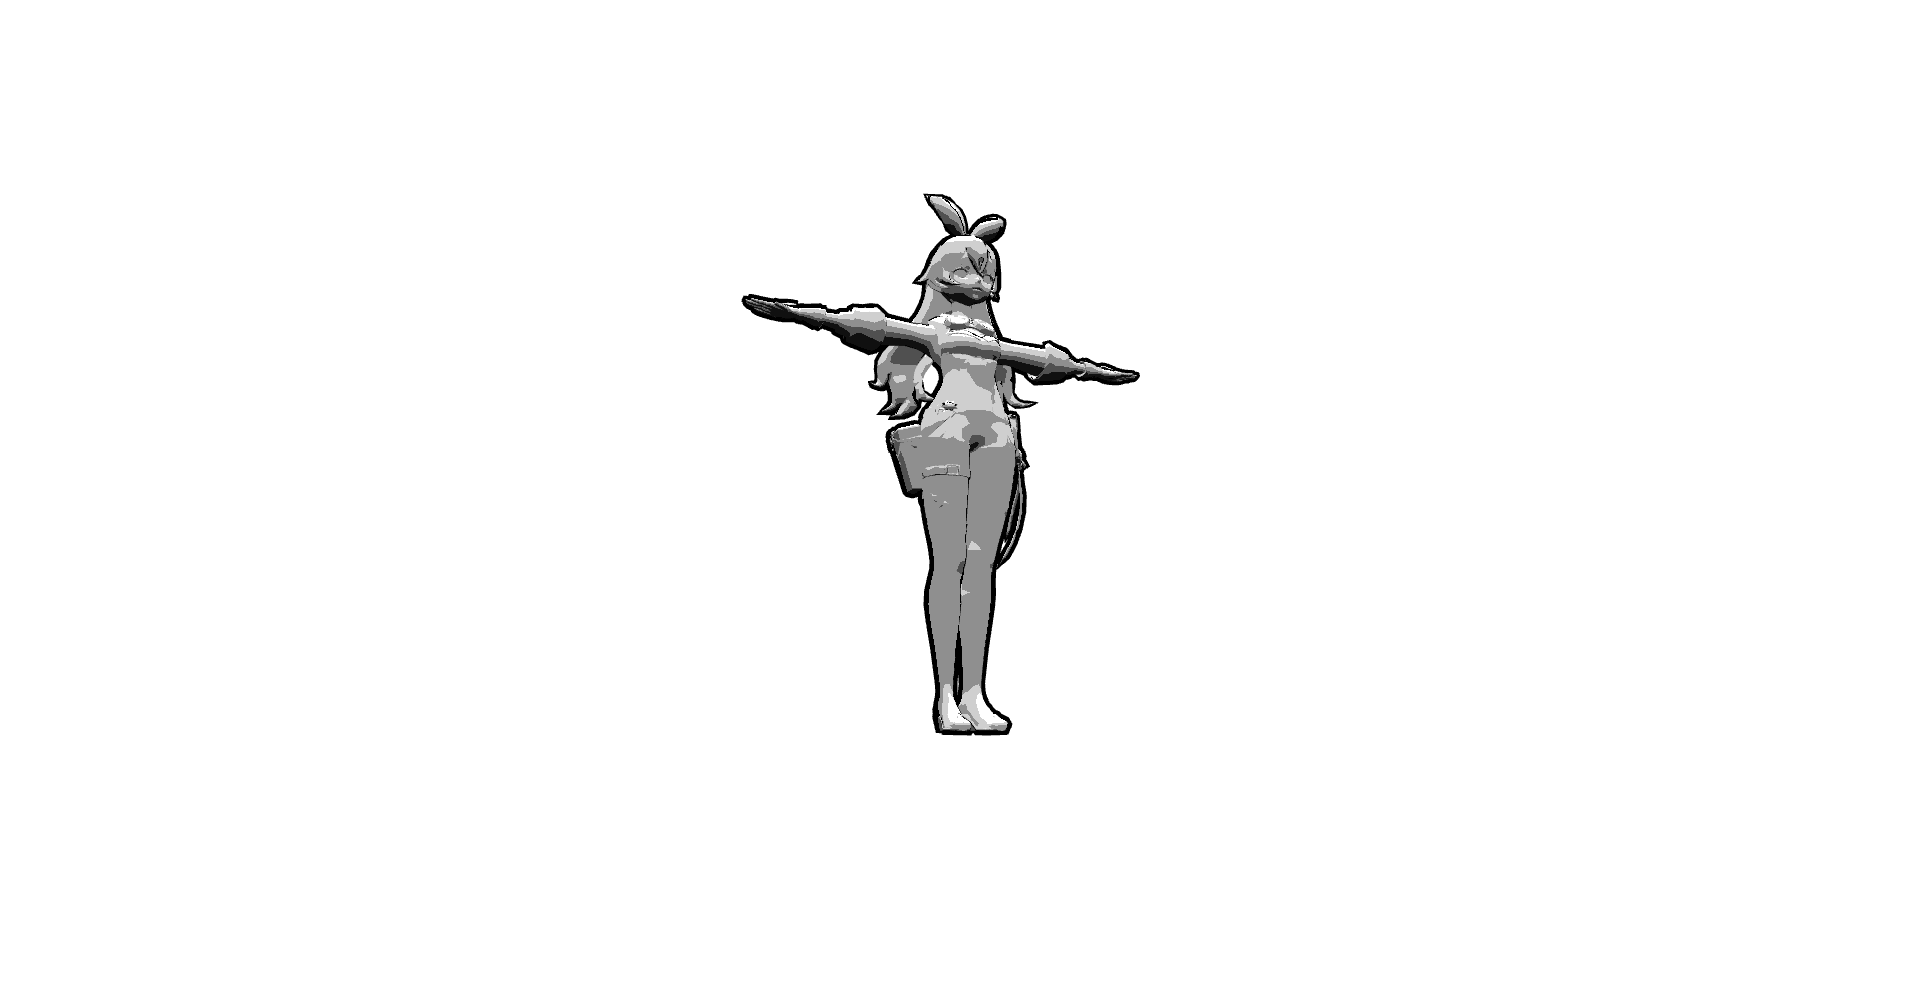
\includegraphics[width=1\linewidth]{amber/base.png}}
        \caption{Amber drawn without suggestive contours.}
        \label{fig:amber-base}
    \end{subfigure}
    \hfill
    \begin{subfigure}{.48\linewidth}
        \frame{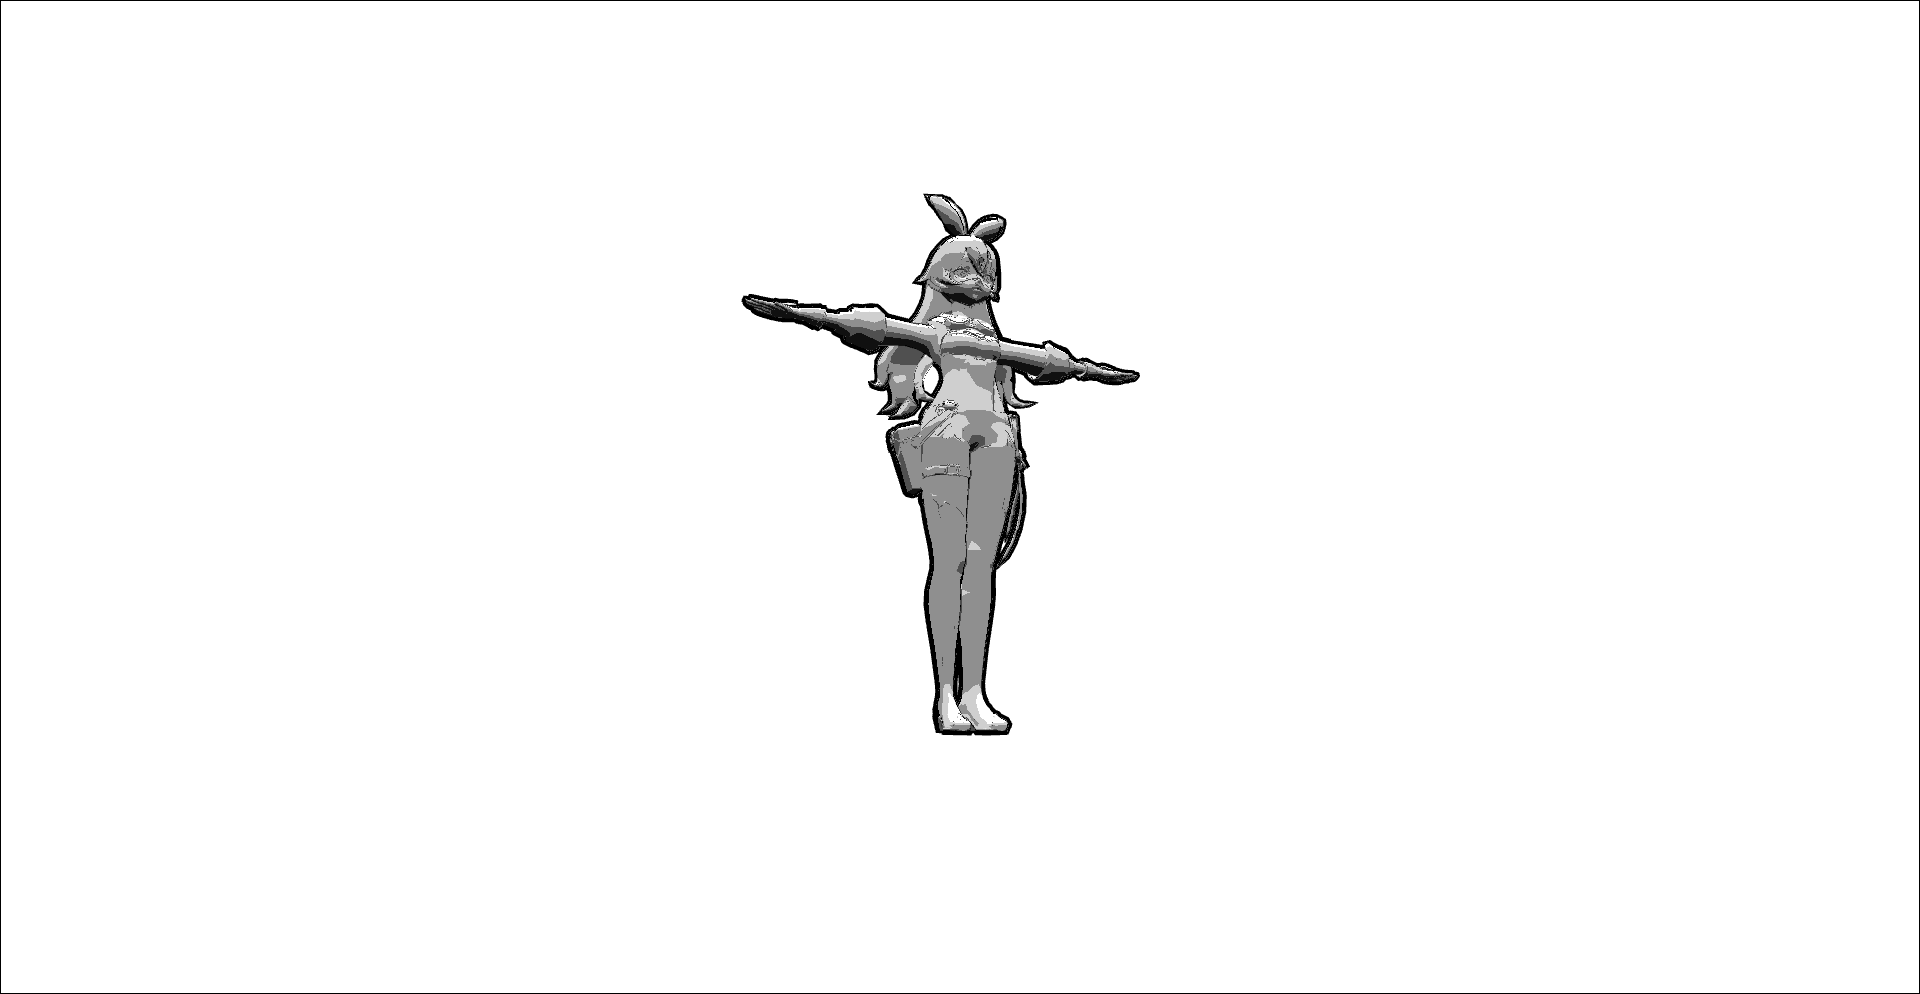
\includegraphics[width=1\linewidth]{amber/final.png}}
        \caption{Amber drawn with suggestive contours.}
        \label{fig:amber-final}
    \end{subfigure}
    \caption{Comparing Amber drawn with all nonphotorealistic shading techniques with and without suggestive contours to see which result creates a more cortoon-ish image.}
    \label{fig:amber-compare}
\end{figure*}

%--Pekora Comparison--
\begin{figure*}
    \centering
    \begin{subfigure}{.48\linewidth}
        \frame{\includegraphics[width=1\linewidth]{pekora/base.png}}
        \caption{Pekora drawn without suggestive contours.}
        \label{fig:pekora-base}
    \end{subfigure}
    \hfill
    \begin{subfigure}{.48\linewidth}
        \frame{\includegraphics[width=1\linewidth]{pekora/final.png}}
        \caption{Pekora drawn with suggestive contours.}
        \label{fig:pekora-final}
    \end{subfigure}
    \caption{Comparing Pekora drawn with all nonphotorealistic shading techniques with and without suggestive contours to see which result creates a more cortoon-ish image.}
    \label{fig:pekora-compare}
\end{figure*}


\end{document}
